\documentclass[14pt]{extarticle}
\usepackage[utf8]{inputenc}  % Korrekt håndtering af æ, ø og å 
\usepackage[T1]{fontenc}  % Korrekt håndtering af æ, ø og å 
\usepackage{microtype}  % Typografisk magi! Giver bl.a. pænere orddeling 
\usepackage{graphicx} % Gør det muligt at indsætte billeder  
\usepackage{amsmath}  % Giver adgang til uundværlige matematikting  
\usepackage{mathtools}
\usepackage{amssymb}
\usepackage{helvet}
\usepackage{revsymb}

\usepackage{bm} % Bold math
\usepackage[natbib=true, 
            style=numeric,
            sorting=none]{biblatex} % Referencer 
\addbibresource{ref.bib}

\usepackage{parskip}

\setlength\parindent{0pt} %stopper indentering ved nyt paragraf 
\usepackage{dsfont} 
\usepackage{subcaption}
\usepackage{caption}

\usepackage{enumitem} %giver ekstra funktionalitet til enumerate og itemize 
				    % fx [label=(\roman*), labelsep=0pt, labelwidth=0pt, labelindent=0pt, itemindent=0pt, topsep=0pt, itemsep=0pt]

\usepackage{xcolor} 	%\textcolor{color}{text} for farvet text 
				%\colorbox{color}{content} for baggrundsfarve 
				%\textcolor{blue!50!white}{text} for at blande farver til finjustering 

\usepackage{geometry} % leger med marginer og andre ting ved dokumentet
\geometry{margin=1.25in} % duh
%\renewcommand{\thesection}{\Alph{section}}
% her erstattes alph med f.eks. Alph, arabic, roman eller Roman og ) kan fjernes eller erstattes

\usepackage{wrapfig}
\usepackage[skip=2pt,font=footnotesize]{caption}

\newcommand{\ds}{\displaystyle} 

\newcommand{\la}{\langle} 
\newcommand{\ra}{\rangle} 

\renewcommand{\v}{\left} 
\newcommand{\h}{\right} 

\usepackage{titlesec}

\titleformat{\section}
  {\normalfont\fontsize{16}{15}\bfseries}{\thesection}{1em}{}

\titleformat{\subsection}
  {\normalfont\fontsize{14}{15}\bfseries}{\thesubsection}{1em}{}

\titleformat{\subsubsection}
  {\normalfont\fontsize{12}{15}\bfseries}{\thesubsubsection}{1em}{}


\begin{document}

%\include{Titlepage}

%\maketitle
\pagenumbering{roman}
\tableofcontents

\newpage
\pagenumbering{arabic}
%\input{Preface}
\setcounter{page}{1}

%
\section{Content ideas}

\begin{itemize}
    \item Introduction
    \item Theory
    \subitem - Light/matter interaction
    \subitem - Single mode optical cavity
    \subitem - The membrane/grating (mechanical and optical properties) 
    \subitem - The Fabry-Perot interferometer
    \subitem - Fano theory (formally) 
    \subitem - The single Fano cavity + simulations
    \subitem - The double Fano cavity + simulations
    \subitem - Optomechanics (?)
    \item Experiment
    \subitem - Sub-wavelength optical grating
    \subitem - Single Fano cavity
    \subitem - Double Fano cavity
    \subitem - Mechanical measurements
    \item Results/Discussion
\end{itemize}


\newpage
\newpage
\section{Introduction}

Cavity electrodynamics is the study of light confined inside an optical resonater and, in the case of this project, quantized as a basis of harmonic oscillator modes. The quantization of the electromagnetic (EM) field inside an optical cavity has been, and continues to be, paramount in the advancement of fields such as optical communication, quantum optics, photonics, sensing, optomechanics, etc. The ability to enhance mode selection of a coherent light source allows for an increase in control of a given system, and highly resolved measurements. 

Many different types of resonators and materials have been utilized for cavity electrodynamics, e.g. beams, drums, photonic crystals and membranes. The latter is here of specific interest, as low mass \emph{Silicon Nitride (SiN)} membranes have proven to posses low losses in the visible- and infrared spectral ranges, and has furthermore been shown to have excellent mechanical properties. Examples of applications of $SiN$ membranes as mechanical resonators used in cavity electrodynamics are as transducers between optical and microwave fields in telecommunication and in sensing for accelerometry, thermometry and pressure sensing. 

However, while $SiN$ membranes are great mechanical resonators, they typically display relatively low reflectivities of $\sim 10\%$ - $35\%$. That is when only the bare membrane is considered. In order to preserve the quality of the mechanical properties along with the low mass, while achieving higher values for the reflectivity, the membranes are patterned with periodic sub-wavelength, 1- or 2-dimensional, photonic crystal structures. In the past decade, tremendous strides have been made in the field of micro- and nano-fabrication methods, and patterned membranes with a record reflectivity of as high as $\sim 99.9998\%$ have been reported.

The type of patterned membrane considered for this project is a 1-dimensional sub-wavelength grating with optical properties well-described by the theory presented by Fan and Joannopoulos \cite{Fan-Joannopoulos-guided-mode-resonance} \cite{Fan-Joannopoulos-fano-resonance}. It is thus said to act as so-called \emph{Fano mirrors} with transmission and reflection coefficients dependent on the incident wavelength. The wavelength-dependence gives rise to a \emph{guided-mode} resonance which can bu utilized in the designing of optical \emph{Fano} cavities with spectra showcasing ultra-narrow linewidth resonance peaks. By tuning the cavity mode and incoming EM-field to match the guided-mode, one can resolve structures with a linewidth in the low picometer regime for cavity lengths down to a few microns. 

In previous work, the single Fano cavity has been realized and characterized, consisting of a broadband mirror and a Fano mirror in a plane-plane configuration. The Fano cavity have proved to produce ultra-narrow linewidth resonance spectra for very short cavity lengths, while still maintaining a high radiation pressure and thus mechanical Q-factor. This makes them an excellent candidate as subjects for optomechanical experiments and corresponding sensing applications. 

In this project we propose the \emph{double Fano cavity} as an expansion of the theory presented for the single Fano cavity by Mitra et al. in \cite{Mitra}. The double Fano cavity consists of two Fano mirrors with each their wavelength-dependent set of optical coefficients and will thus, theoretically, produce an even narrower resonance profile than the \emph{single} Fano cavity. Figure \ref{fig:all_cavities_sketch} shows schematics for all three aforementioned optical cavities, namely the broadband cavity (\ref{fig:broadband_cavity_sketch}), single Fano cavity (\ref{fig:single_fano_cavity_sketch}) and double Fano cavity (\ref{fig:double_fano_cavity_sketch}), where $t_g, r_g$ refers to transmission- and reflection coefficients of a Fano mirror, and $t_m, r_m$ are the ones for a broadband mirror.

\begin{figure}[h!]
    \centering
    \begin{subfigure}[b]{0.3\textwidth}
        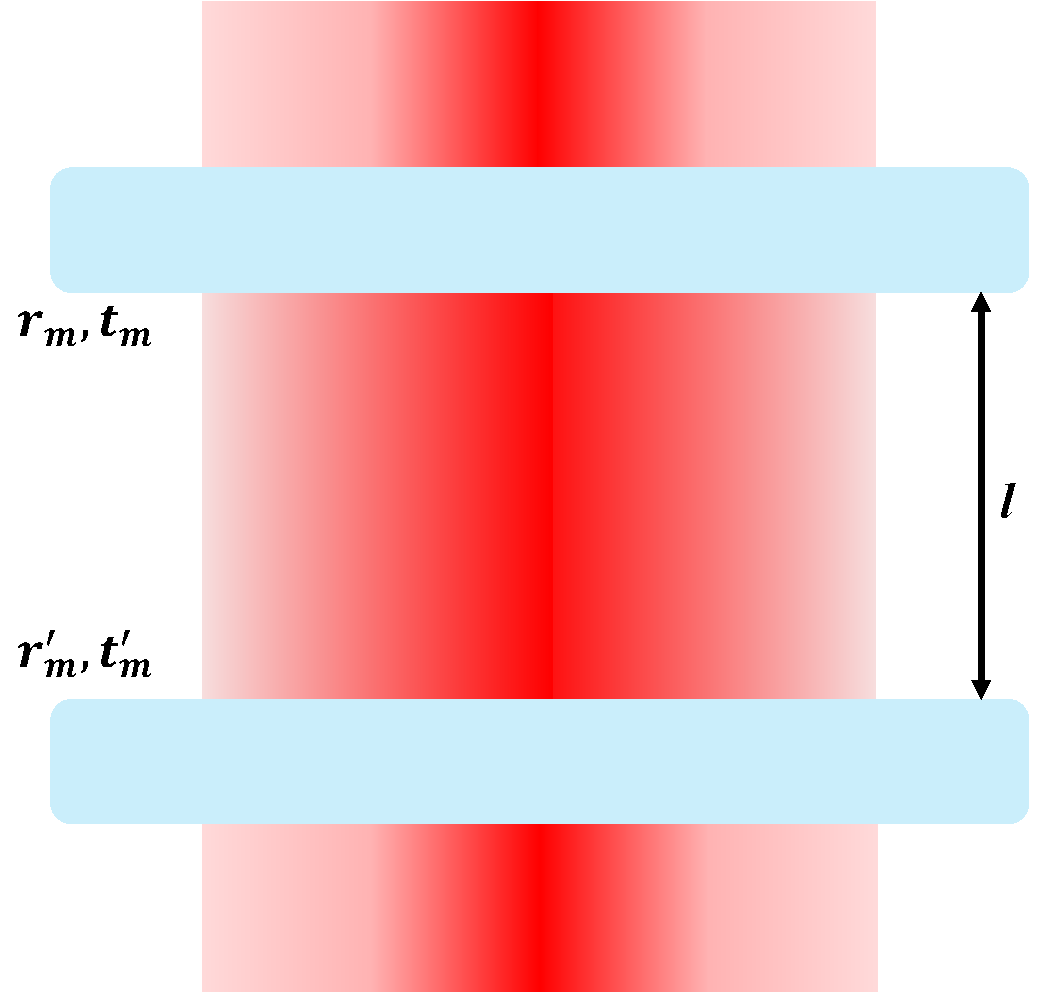
\includegraphics[width=\textwidth]{figures/broadband_sketch.pdf}
        \caption{Broadband cavity.}
        \label{fig:broadband_cavity_sketch}
    \end{subfigure}
    \hfill
    \begin{subfigure}[b]{0.3\textwidth}
        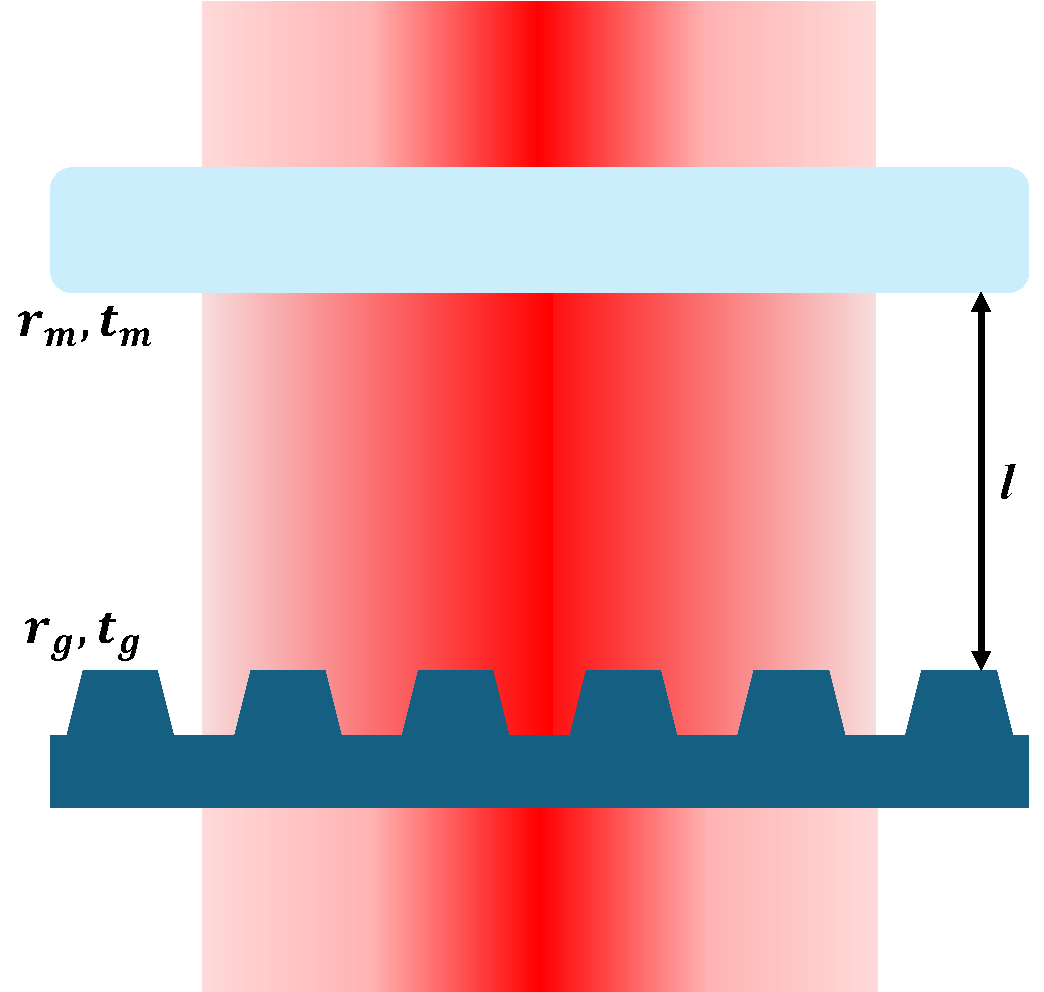
\includegraphics[width=\textwidth]{figures/single_fano_sketch.pdf}
        \caption{Single Fano cavity.}
        \label{fig:single_fano_cavity_sketch}
    \end{subfigure}
    \hfill
    \begin{subfigure}[b]{0.3\textwidth}
        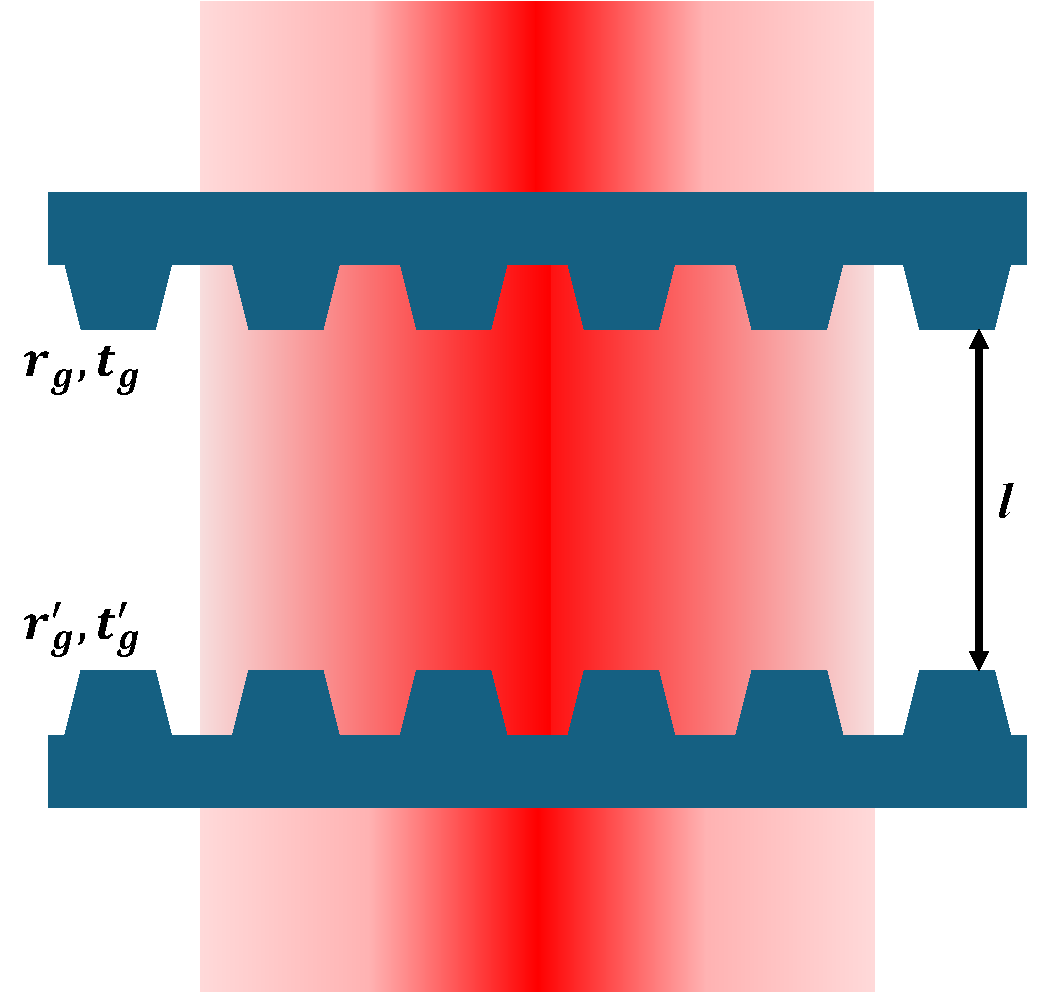
\includegraphics[width=\textwidth]{figures/double_fano_sketch.pdf}
        \caption{Double Fano cavity.}
        \label{fig:double_fano_cavity_sketch}
    \end{subfigure}
    \caption{}
    \label{fig:all_cavities_sketch}
\end{figure}

In this thesis I will present the theory of the sub-wavelength grating, i.e. Fano mirrors, and of the single- and double Fano cavities. I will show extensive simulations run for the transmission spectra of the double Fano cavity as a part of my investigations in order to map the on- and off-resonance behaviour as functions of various physical parameters. I will expand in detail on the experimental methods and techniques used in order to realize said theory and outline obstacles faced in that process. Finally I will present the results of my project and compare these with analytical predictions and discuss shortcomings and sources of error and noise of the setup and methods used. I will end by briefly dicussing the possible outlook of future projects regarding the double Fano cavity and the field of cavity electrodynamics generally in the light of my findings. 

\newpage
\section*{Theory}
\section{Theory}
\subsection{The Fabry-Perot interferometer}\label{sec:fabry_perot}

The Fabry-Perot interferometer, also known as an optical cavity, is generally comprised of two reflective optical elements, hereafter refered to as mirrors. In the following we assume a plane-plane configuration for two lossless mirrors and a plane-wave at normal incidence for the incoming field, as sketched in figure \ref{fig:planar_fabry-perot}. 

\begin{figure}[h!]
    \centering
    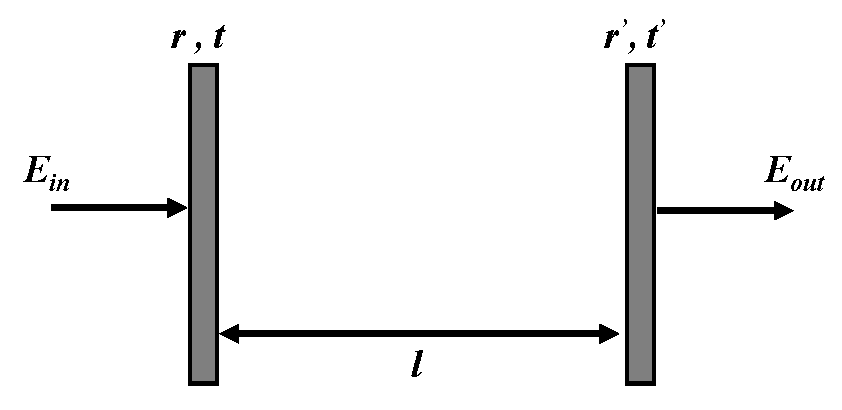
\includegraphics[width=0.6\textwidth]{figures/planar_fabry_perot.pdf}
    \caption{Sketch of a planar Fabry-Perot cavity.}
    \label{fig:planar_fabry-perot}
\end{figure}

The two mirrors are described by each their respective reflectivity \emph{r} and transmission \emph{t} and are placed parallel at a distance \emph{l} from each other. The field at the second mirror, i.e. the transmitted field $E_{out}$ can then be described as a function of the field at the first mirror, i.e. the incident field $E_{in}$\cite{Eichhorn} \cite{Pedrotti}. The Fabry-Perot cavity furthermore gives rise to so-called eigenstates related to it's length \emph{l}, derived from considering the path difference between succesive parallel beams throught the cavity. Any allowed mode inside the cavity, and thus transmitted, must fulfill the brightness condition $2l = m \lambda$, where $\lambda$ is the wavelength of the incident field and $m=1,2,3,...$ is a positive integer.  

\subsubsection{Transmission}

In order to determine the transmission throught the Fabry-Perot interferometer, we once again consider the configuration in figure \ref{fig:planar_fabry-perot}. It is further, initially, assumed that resonators are both lossless, such that
\begin{equation}
    |r|^2 + |t|^2 = |r^{\prime}|^2 + |t^{\prime}|^2 = 1.
    \label{eq:lossless_condition}
\end{equation}

This means that all losses, e.g. absorption, are neglected. 

In order to formulate the field transmitted at the 2nd mirror $E_{out}$ in terms of the incident field at the 1st mirror $E_{in}$, we first consider the incident field as a propagating plane-wave
\begin{equation}
    E_{in} = E_{0,in} e^{ik},
\end{equation}

where $k = 2 \pi / \lambda$ is the wave number and $E_{0,in}$ is the amplitude of the field. We then consider $E_{out}$ to be comprised of contributions for each roundtrip inside the cavity. This can be written as an infinite geometrical series given as
\begin{equation}
    \begin{split}
        E_{out} & = tt^{\prime} E_{0,in} e^{ik} + tt^{\prime} E_{0,in} e^{ik} rr^{\prime} e^{i\delta}\\&+ tt^{\prime} E_{0,in} e^{ik} \left(rr^{\prime} e^{i\delta}\right)^2 + tt^{\prime} E_{0,in} e^{ik} \left(rr^{\prime} e^{i\delta}\right)^3 + ...\\& = tt^{\prime} E_{0,in} e^{ik} \sum^{\infty}_{m=0}\left( rr^{\prime}e^{i\delta} \right)^m
    \end{split}
    \label{eq:transmission_as_geometric_series}
\end{equation}
where $\delta = 2kl$. The first term of the series corresponds to a direct transmission through the cavity, and each term thereafter corresponds to the respective contribution to the transmission after the $m'th$ round trip. 

By evaluating the series it is seen that it converges to the final expression for the transmitted field through a planar Fabry-Perot cavity found as
\begin{equation}
    E_{out} = E_{0,in}\frac{tt^{\prime} e^{i\delta /2}}{1 - rr^{\prime} e^{i\delta}}.
    \label{eq:fabry_perot_trans}
\end{equation}

The intensity of the transmission is now taken as the square of the norm of the field amplitude $|E_{out}|^2$ and normalizing with respect to the incident field intensity $|E_{0,in}|^2$ we arrive at an expression for the transmission intensity which is recognized to be given as an \emph{Airy function}\cite{Pedrotti}
\begin{equation}
    T = \frac{|E_{out}|^2}{|E_{0,in}|^2} = \left|\frac{tt^{\prime}e^{i\delta/2}}{1 - rr^{\prime}e^{i \delta}}\right|^2 = \frac{(1-|r|^2)(1-|r^{\prime}|^2)}{(1-|rr^{\prime}|)^2 + 4|rr^{\prime}|sin^2(\delta)},
    \label{eq:airy_function}
\end{equation}
where $\delta$ is the phase shift for each round trip inside the cavity.

\begin{figure}[h!]
    \centering
    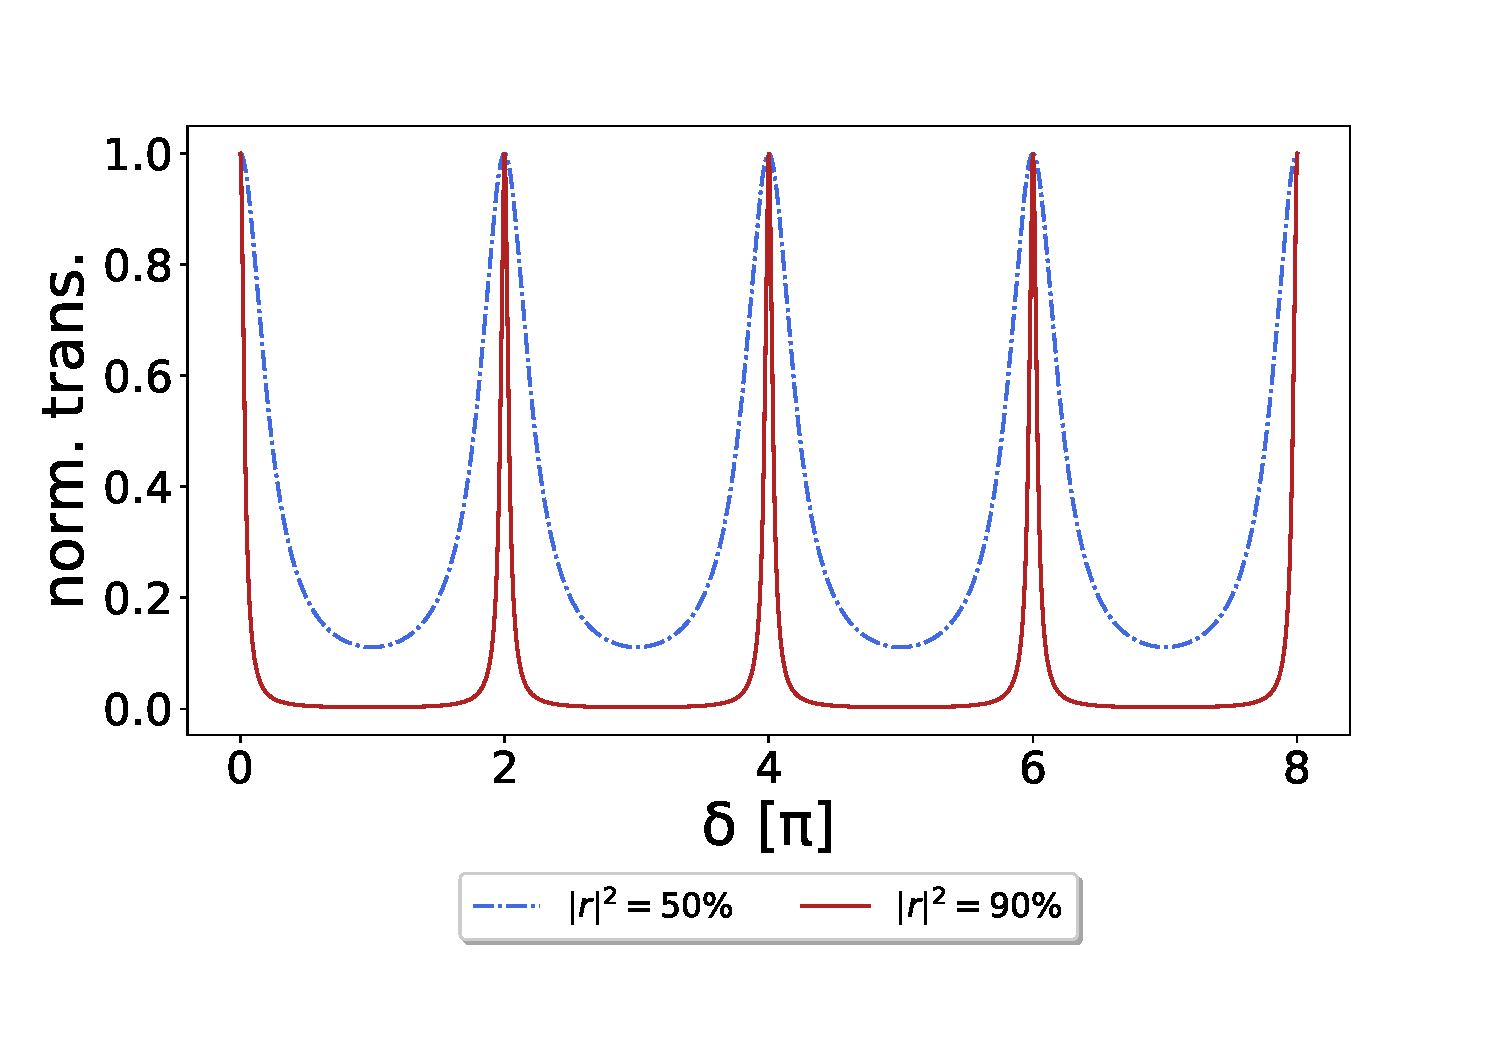
\includegraphics[width=0.7\textwidth]{figures/fabry_perot_high_and_low_finesse.pdf}
    \caption{The red line shows the transmission spectrum of a \emph{high} finesse Fabry-Perot cavity of reflectivity $|r|^2 = 0.90$, while the blue dashed line shows the transmission spectrum of a \emph{low} finesse cavity with reflectivity $|r|^2 = 0.50$.}
    \label{fig:fabry_perot_trans}
\end{figure}

Figure \ref{fig:fabry_perot_trans} displays the Airy function in eq. (\ref{eq:airy_function}), of a lossless cavity of reflectivities $r^{\prime} = r$, as a function of $\delta$ in units of $\pi$. The function is plotted for the cases of $|r|^2 = 50 \%$, shown in blue, and $|r|^2 = 90 \%$, shown in red. It is readily seen that the transmission is maximized for $\delta = n 2 \pi$ and that the two cases shown differ significantly as the red profile is much narrower than the blue. The red profile is hence said to have a higher \emph{finesse} $\mathcal{F}$ than the blue profile. The finesse is defined as
\begin{equation}
    \mathcal{F} \equiv \frac{FSR}{\delta_{\lambda}},
    \label{eq:finesse_definition}
\end{equation}
where $FSR$ is the so-called \emph{Free Spectral Range} indicating the spectral distance between two peaks and $\delta_{\lambda}$ refers to the \emph{Full Width at Half Maximum (FWHM)} which, as the name suggests, is the linewidth defined at $T=1/2$, i.e. at half the maximum value. 

Considering the Airy function in eq. (\ref{eq:airy_function}) for the high finesse case where $|r|^2 = |r^{\prime}|^2 \rightarrow 1$ we furthermore see that each individual peak resembles a Lorentzian distribution. 

\subsubsection{Varying the cavity length}

In order to relate the resonance transmission profile to the length of the cavity we first consider the frequencies at which the cavity is resonant, with respect to the incident light, given as
\begin{equation}
    \nu_n = n \frac{c}{2l},
    \label{eq:resonance_freq}
\end{equation}
where $c$ is the speed of light, $n$ is a positive integer refering to the order of the resonance frequency and $l$ is the cavity length. This corresponds to a peak occuring at times related to each round trip inside the cavity. 

Since the FSR is defined as the spectral distance between each peak, it follows from eq. (\ref{eq:resonance_freq}) that it can be be expressed in terms of the resonance frequencies as 
\begin{equation}
    FSR_{\nu} = \frac{c}{2l},
    \label{eq:FSR_vs_cavity_length}
\end{equation}
and the corresponding linewidth, or FWHM, $\delta_{\nu}$ is then given as
\begin{equation}
    \delta_{\nu} = \frac{1}{2 \pi} \frac{|t|^2 + |t^{\prime}|^2}{\tau},
\end{equation}
where $\tau = 2l/c$ is the round trip time in seconds. 

Finally, considering the definition of the finesse from eq. (\ref{eq:finesse_definition}) it can be shown that
\begin{equation}
    \mathcal{F} \equiv \frac{FSR_{\nu}}{\delta_{\nu}} = \frac{2 \pi}{|t|^2 + |t^{\prime}|^2},
    \label{eq:lossless_finesse}
\end{equation}
where the finesse is now defined in terms of the total cavity transmission at resonance. 

Note here that the relation between the FSR and the cavity length $l$ is clearly shown in eq. (\ref{eq:FSR_vs_cavity_length}), and figure \ref{fig:fabry_perot_FSR_comparison} furthermore shows transmission spectra underlining the effect of changing the cavity length. 

\begin{figure}[h!]
    \centering
    \begin{subfigure}[b]{0.49\textwidth}
        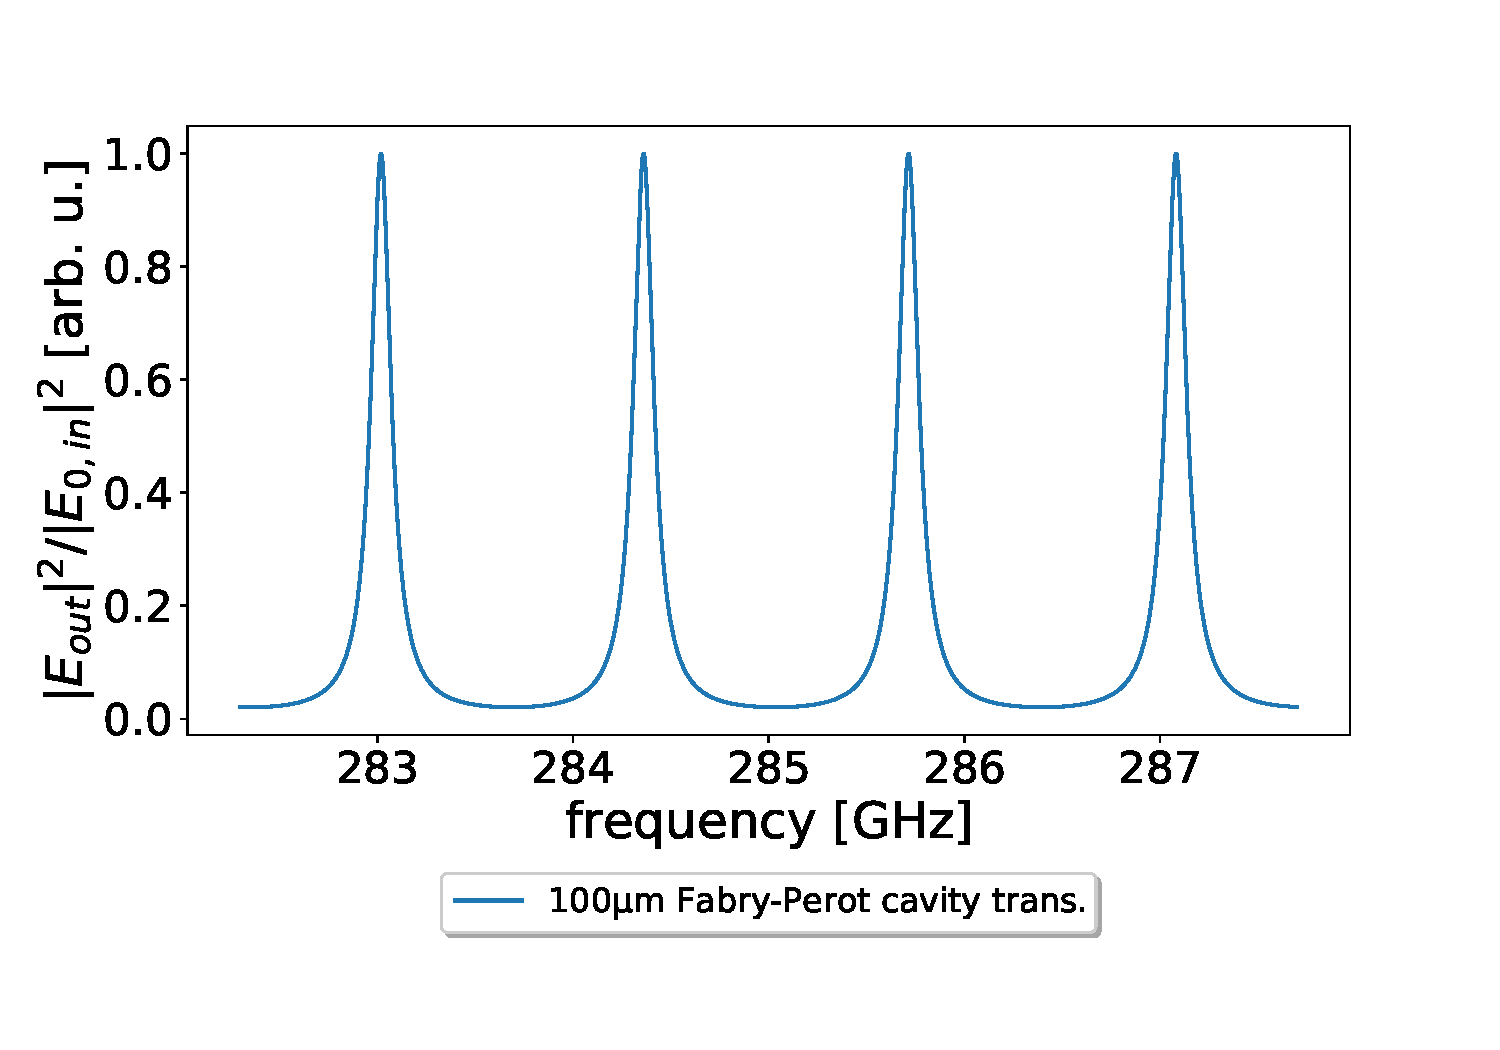
\includegraphics[width=\textwidth]{figures/100um_fabry_perot_trans_vs_freq.pdf}
        \caption{}
    \end{subfigure}
    \begin{subfigure}[b]{0.49\textwidth}
        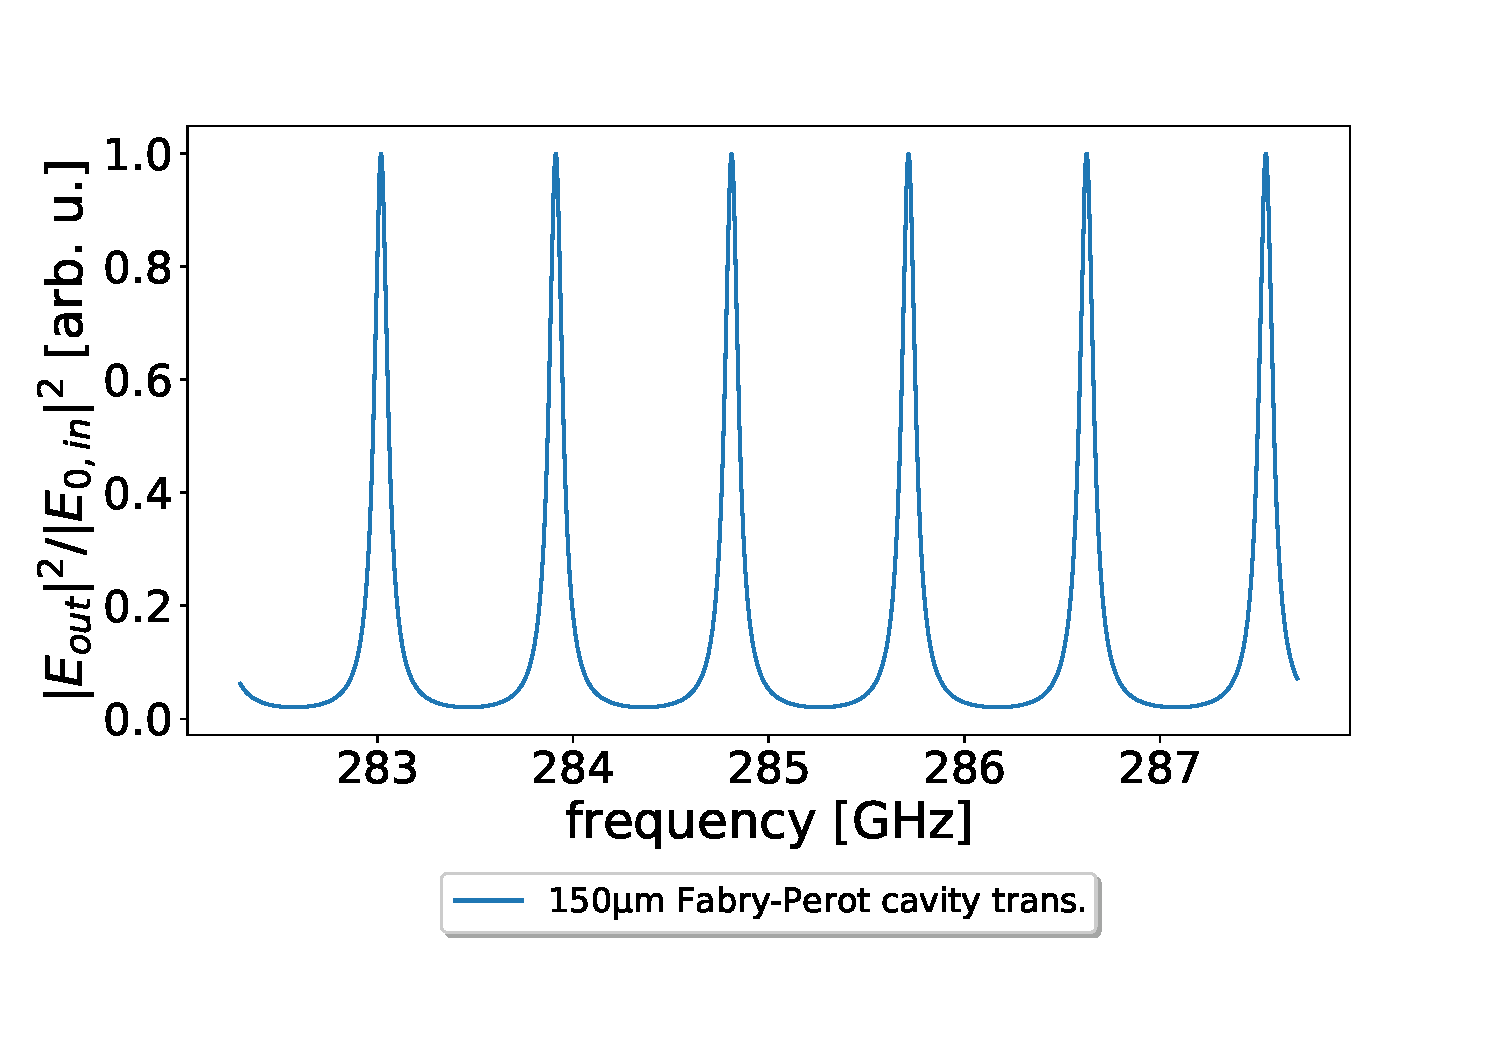
\includegraphics[width=\textwidth]{figures/150um_fabry_perot_trans_vs_freq.pdf}
        \caption{}
    \end{subfigure}
    \caption{(a) shows the transmission spectrum of a Fabry-Perot cavity of length $l \approx 100 \mu m$ as a function of the frequency $\nu$, while (b) shows the transmission spectrum of a cavity of length $l \approx 150 \mu m$ for the same range of frequencies. Note here how the FSR is invrsely proportional to the cavity length.}
    \label{fig:fabry_perot_FSR_comparison}
\end{figure}

\subsubsection{Varying the incident wavelength}

In order to simplify the Airy function in eq. (\ref{eq:airy_function}) we introduce the so-called \emph{coefficient of finesse} $F$, which is a function only of the mirror reflectivites, given as
\begin{equation}
    F = \frac{4 |rr^{\prime}|}{(1-|rr^{\prime}|)^2}.
\end{equation}

The coefficient of finess $F$ is not to be confused with the finesse $\mathcal{F}$. While the finesse is related to the sharpness of the transmission peaks, the coefficient of finesse refers to the contrast of the peaks in the sense that the difference between the minimum and maximum transmitance level increases with $F$. The coefficient of finesse is related to the finesse as 
\begin{equation}
    \mathcal{F} = \frac{\pi}{2} \sqrt{F}.
\end{equation}

Rewriting the Airy function in terms of the coefficient of finesse yields
\begin{equation}
    T_{\lambda} = \frac{1}{1+ F sin^2 \left(\delta / 2\right)},
\end{equation}
where the round trip phase shift $\delta$ is related to the wavelength $\lambda$ of the incident light by
\begin{equation}
    \delta = 2kl = \frac{4 \pi l }{\lambda},
\end{equation}
as $k = 2 \pi / \lambda$ is the incident wave number.

Re-writing the general cavity brightness condition, it can be shown that the resonant wavelengths for a cavity at normal incident are given as
\begin{equation}
    \lambda_n = \frac{2l}{n},
\end{equation}
where $n=1,2,3,...$ is a positive integer refering to the order of the resonance. 

Since $\nu = c / \lambda$, the relation between the linewidth in wavelength space $\delta_{\lambda}$ and the one in frequency space $\delta_{\nu}$ is non-linear. Therefore one does not simply make the aforementioned substitution in order to relate them. It can however be shown that their respective expressions differ by a factor of $\lambda^2/c$, and the linewidth when varying the wavelength is thus given as
\begin{equation}
    \delta_{\lambda} = \frac{\lambda^2}{c} \cdot \delta_{\nu} = \frac{\lambda^2}{4 \pi l} (|t|^2 + |t^{\prime}|^2).
\end{equation}
Finally we consider the definition for the finesse $\mathcal{F}$ and the expression given in eq. (\ref{eq:lossless_finesse}), in order to show that the $FSR$ in wavelength space is given as 
\begin{equation}
    FSR_{\lambda} = \delta_{\lambda} \cdot \mathcal{F} =  \frac{\lambda^2}{2l}.
\end{equation}



\begin{figure}[h!]
    \centering
    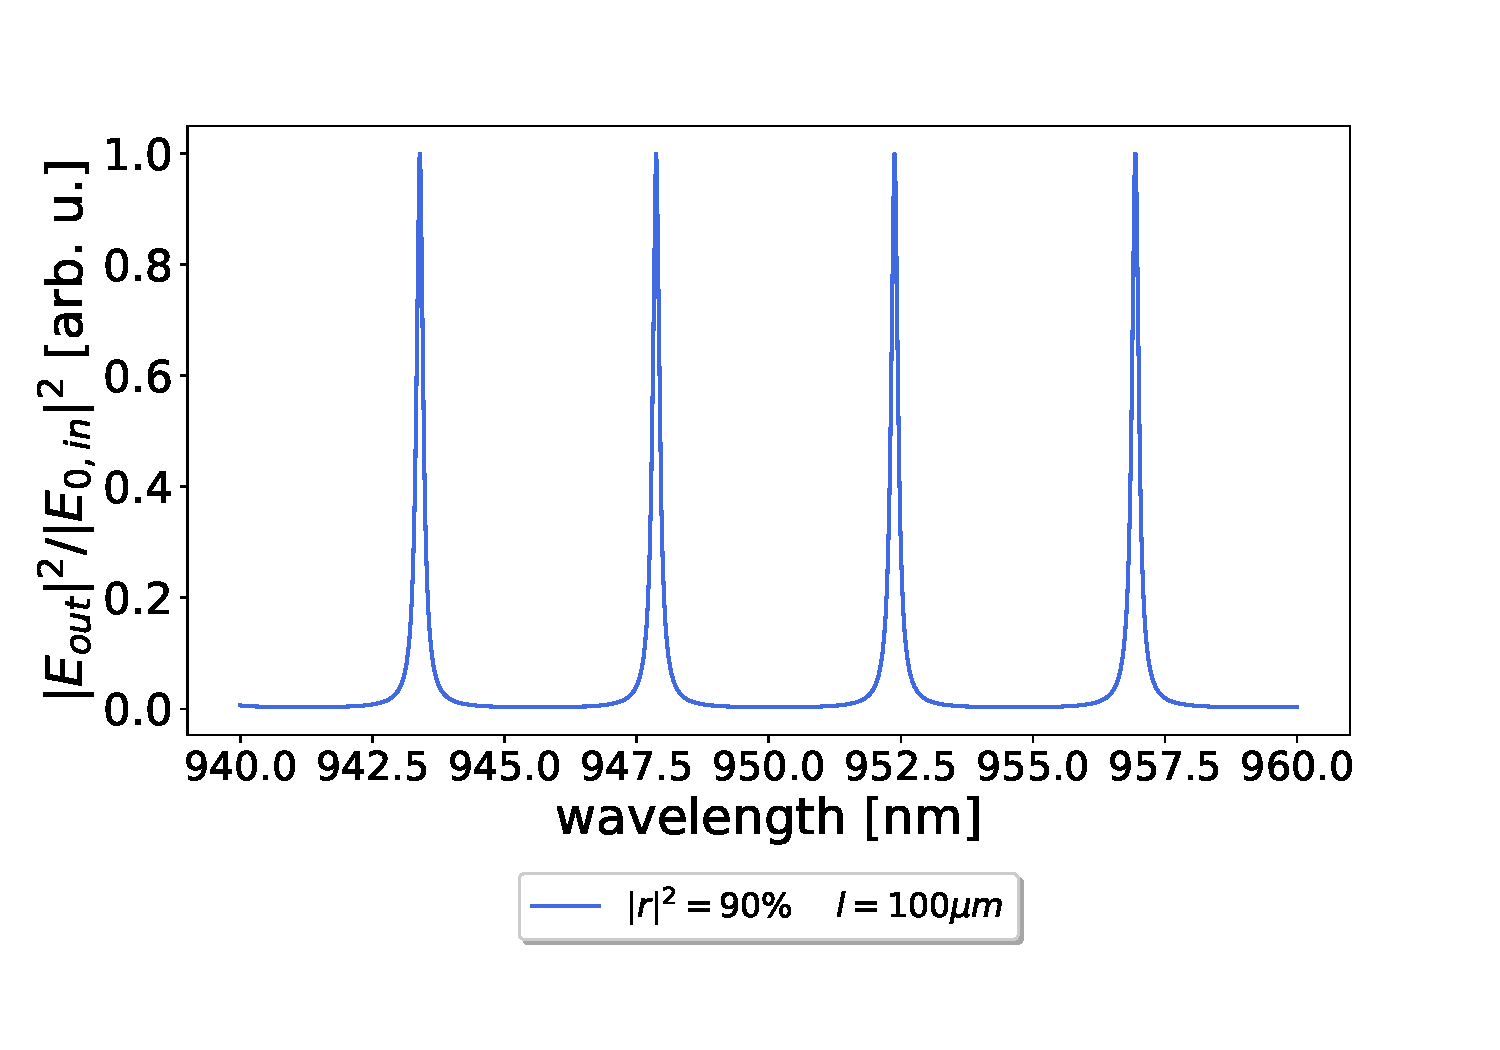
\includegraphics[width=0.7\textwidth]{figures/airy_function_vs_wavelength.pdf}
    \caption{}
    \label{fig:airy_trans_vs_wavelength}
\end{figure}

\subsubsection{Cavity losses}

In eq. (\ref{eq:lossless_finesse}) we assume the case of a lossless cavity, i.e. eq. (\ref{eq:lossless_condition}) is fulfilled. In practice, any cavity will have some amount of losses, which would have to be taken into account when calculating the finesse. When losses are present eq. (\ref{eq:lossless_condition}) instead generally reads
\begin{eqnarray}
    |r|^2 + |t|^2 + L + L^{\prime} = 1,
\end{eqnarray}
where $L$ and $L^{\prime}$ indicates the fractional losses of each resonator.

In this case the finesse would be given as 
\begin{equation}
    \mathcal{F} = \frac{2 \pi}{|t|^2 + |t^{\prime}|^2 + L_{total}},
\end{equation}
where $L_{total} = L + L^{\prime}$ are the total cavity losses.

The effect on the transmission spectrum of a cavity with losses is that the level of the normalized transmission will not reach unity, as some light is lost to i.g. absorption or scattering for each round trip of the cavity.

\subsection{The Fano mirror: a sub wavelength grating}\label{sec:fano_mirror}

\subsubsection{Reflection/transmission spectra and line shape analysis}

\subsubsection{Lossless grating}

We wish to analytically describe the wavelength-dependent spectra for the transmission and reflectivity of an infinite sub-wavelength grating. The wavelength dependence arises from the fact that any incident light will be subject to interactions with the so-called \emph{guided-mode} of the grating. The grating is, in this way, said to act as an effective $\text{TM}_0$ waveguide, ensuring resonant modes will only be reflected in the 0'th order. 

By first considering the case where absorption and thermal coupling effects are neglected, i.e. a lossless grating, we can assume conservation of energy and thereby the relations
\begin{equation}
    |r_g|^2+|t_g|^2=1 \hspace{0.5cm} \text{and} \hspace{0.5cm} |r_d|^2+|t_d|^2=1,
    \label{eq:energy conservation}
\end{equation}
where the subscripts \emph{g} and \emph{d} indicate the \emph{grating} and \emph{direct} transmissions and reflectivities, respectively. It is implied that the direct coefficients are constants and describe the transmission and reflectivity when the incident wavelength is significantly detuned from any guided-mode resonance of the grating. Furthermore, it is also implied that the grating coefficients are functions of the incident wavelength.

We now assume a normal incident beam on the grating as a linearly polarized monochromatic plane wave, with a wavelength close to a guided-mode resonance of the grating. In order to describe the coefficients $r_g$ and $t_g$ we follow the formalism presented by Fan and Joannopoulos \cite{Fan-Joannopoulos-guided-mode-resonance} and consider the likely paths of the incident light through the grating. It is quite intuitive to consider the case where the light is simply transmitted, and this shall be our first case hereafter denoted the \emph{direct pathway}. Another case one might consider is the one where the incident light excites the guided-mode resonance in the grating. This case is denoted the \emph{indirect pathway} and decays more slowly than it's direct counterpart. 

The interference caused when the guided mode is excited is often referred to as \emph{Fano resonances}, due to its physical similarities to the description of interference between a discrete autoionized state and a bound continuum state first reported by Fano \cite{Fano-theory}. The cross section of inelastic scattering, when measured as a function of energy, showed characteristic asymmetric peaks. These were described as the aforementioned interference pattern between \emph{direct} (the discrete state) and \emph{indirect} (the continuum state) pathways. 

By generalizing the model of Fan and Joannopoulos \cite{Fan-Joannopoulos-guided-mode-resonance} we describe the transmission and reflectivity coefficent amplitudes as 
\begin{equation}
    r_g = r_d + \frac{a}{k-k_1 + i\gamma} \hspace{0.5cm} \text{and} \hspace{0.5cm} t_g = t_d + \frac{b}{k-k_1+i\gamma},
    \label{eq:ref/trans}
\end{equation}
where $k=2\pi/\lambda$ is the incident wave number, $k_1 = 2\pi/\lambda_1$ is the wave number according to the guided-mode resonance and $\gamma$ is the HWHM (half width at half maximum) of the guided-mode resonance. Complex coefficients $a$ and $b$ describe the interference between the directly transmitted or reflected waves and the guided mode of the grating. 

Note that in eq. (\ref{eq:ref/trans}) the right side of the expression for each coefficient corresponds to the continuum state i.e. the indirect pathway, while the direct transmission and reflection coefficients take the role of the autoionized discrete state, i.e. the direct pathway\cite{Fano-theory}.

As we are dealing with an ideal, lossless, grating, we assume coefficients $a$ and $b$ to be equal, meaning that we specifically assume vertical symmetry throughout the grating. By considering eq. (\ref{eq:energy conservation}) this in turn leads to 
\begin{equation}
    a = b = -i \gamma (t_d + r_d),
\end{equation}
which further yields an expression for the grating transmission amplitude coefficient on the form
\begin{equation}
    t_g = t_d \frac{k - k_0}{k - k_1 + i \gamma}.
    \label{eq:lossless transmission coefficient}
\end{equation}
Here, the newly introduced $k_0 = 2\pi/\lambda_0 = k_1 -i \gamma (r_d/t_d)$ is the zero-transmission/unity-reflectivity wave number.

To generalize eq. (\ref{eq:lossless transmission coefficient}) to include non-unity reflectivity and non-zero transmission, we allow for $a \neq b$\cite{Bykov}\cite{Darki2}\cite{Parthenopoulos}, meaning that the case of vertical asymmetry is included in the model\cite{Popov}. By assuming $r_d,t_d \in \mathbb{R}$, eq. (\ref{eq:energy conservation}) leads to the coupled differential equations
\begin{equation}
    \begin{split}
        &t_d x_a + r_d x_b = 0, \hspace{0.3cm} \text{and} \\
        &x_a^2 + y_a^2 + x_b^2 + y_b^2 + 2 t_d \gamma y_a + 2 r_d \gamma y_b = 0,
    \end{split}
    \label{eq:lossless couples diff. eqs.}
\end{equation}
where $\{x,y\}_{a,b}$ respectively denotes the real and imaginary parts of the coefficients $a$ and $b$. Solving eqs. (\ref{eq:lossless couples diff. eqs.}) leads to the correct complex reflectivity coefficients and the expression for the transmission coefficient amplitudes now reads
\begin{equation}
    t_g = t_d \frac{k - k_0 + i \beta}{k - k_1 + i \gamma},
    \label{eq:transmission_coefficients_non_zero_values}
\end{equation}
where $k_0$ and $\beta$ are defined from the expression for $a$ found by solving eqs. (\ref{eq:lossless couples diff. eqs.}), given as
\begin{equation}
    a = t_d (k_1 - k_0 - i \gamma + i \beta).
\end{equation}
Finally, this allows for non-zero transmission and non-unity reflectivity at wave number $k_0$.

To show the validity of the model at this point, we introduce a periodic grating which is arbitrarily sketched in figure \ref{fig:MIST_grating_sketch}. The sketch indicates the period of the grating $\Lambda$, the top finger width $w_t$, the offset between the finger top and the bottom of the grating $x$, the total grating thickness $t$ and finger depth $d$. Furthermore, the grating is patterned on a \emph{silicon nitride (SiN)} membrane  of refractive index $n_{SiN}$. 

\begin{figure}[h!]
    \centering
    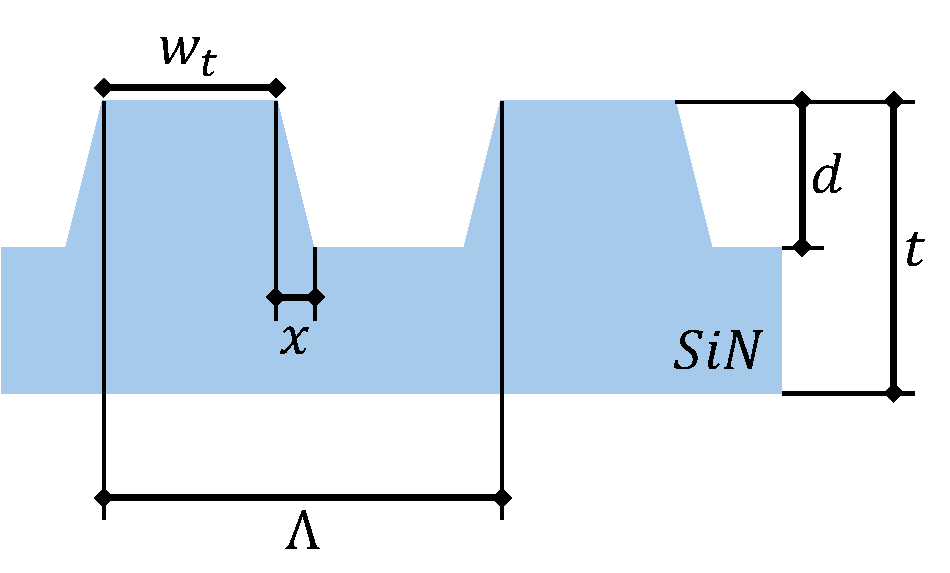
\includegraphics[width=0.7\textwidth]{figures/grating_MIST_sketch.pdf}
    \caption{Schematics of a periodic optical $SiN$ grating with phyiscal parameters: $\Lambda = 857$nm, $w_t = 623$nm, $h = 55.1$nm, $t = 152$nm, $d = 67$nm, $n_{SiN} = 2.15$.}
    \label{fig:MIST_grating_sketch}
\end{figure}


In order to simulate the transmission and reflectivity profiles as a function of the incident wavelength, we utilize the \emph{Modeled Integrated Scatter Tool (MIST)} developed by the \emph{National Institute of Standards and Technology (NIST)}\cite{MIST}. The simulation solves Maxwell's equations for any pre-defined infinite periodic structure. 

MIST assumes an incident plane-wave, and hence predicts the \emph{ideal} spectra for the transmission and reflectivity, i.e. zero and unity when on resonance, respectively. In order to include effects related to the Gaussian behaviour of a more realistic incident beam, such as collimation and finite-size effects\cite{Toft-Vandborg}, one would have to solve Maxwell's equations for a Gaussian distribution. We safely assume an incident plane-wave for reasons related to the order of magnitude for the \emph{Rayleigh range} of the beam used, compared with that of the spacial range of the conducted experiments.

In reality, the interference inside the cavity however cannot be perfect, as any Gaussian beam can be represented by a number rays, infinitesimal in size, which would all track differently through the grating, resulting in non-unity reflectivity and non-zero transmission. In order to synthetically correct for this we scale each transmission value found by MIST according to
\begin{equation}
    t_g = (1 - \varepsilon) \cdot t_{MIST} + \varepsilon,
    \label{eq:trans_correction_MIST}
\end{equation}
where we define the correction to be arbitrarily small as $\varepsilon = 1\%$.

\begin{figure}[h!]
    \centering
    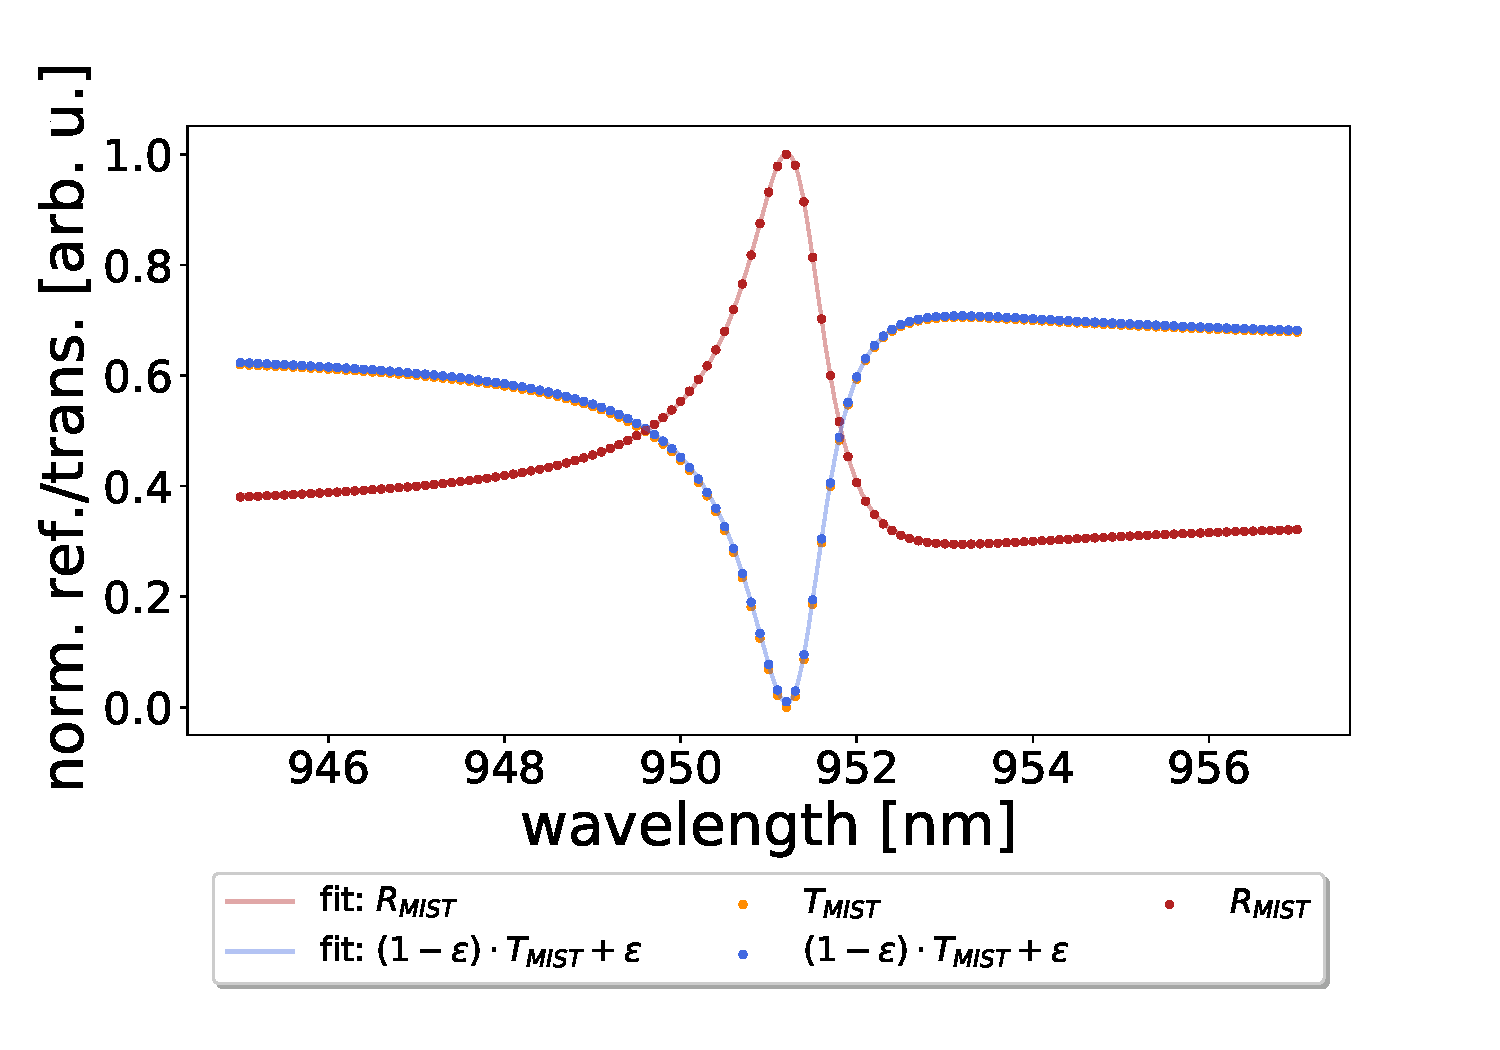
\includegraphics[width=0.7\textwidth]{figures/MIST_grating_sim.pdf}
    \caption{Reflectivity and transmission values (scaled and unscaled) found from a MIST simulation plotted with the corresponding least squares fit to the model in eq. (\ref{eq:transmission_coefficients_non_zero_values}). The resulting grating parameters are given as $\lambda_0 = 951.217$nm, $\lambda_1 = 951.356$nm, $t_d = 0.818$, $r_d = 0.527$, $\gamma_{\lambda} = 0.527$nm, and $\beta = 1.03 \cdot 10^{-6}$.}
    \label{fig:MIST_sim_of_grating}
\end{figure}

Figure \ref{fig:MIST_sim_of_grating} shows the scaled and unscaled results of the simulation using MIST for the following physical grating parameters:
\begin{equation}
    \begin{split}
    &\Lambda = 857 \text{nm},\:\: w_t = 623 \text{nm},\:\: h = 55.1 \text{nm},\\ &t = 152 \text{nm},\:\: d = 67 \text{nm}\: \text{ and }\: n_{SiN} = 2.15,
    \end{split}
    \label{eq:physical_grating_params}
\end{equation}

The reflectivity- and (corrected) transmission values were then fitted to the model in eq. (\ref{eq:transmission_coefficients_non_zero_values}) using a least squares fitting method, and plotted along with the simulated values. The resulting grating parameters were found as
\begin{equation}
    \begin{split}
    &\lambda_0 = 951.208 \text{nm},\:\: \lambda_1 = 951.356 \text{nm},\:\: t_d = 0.8094,\\ &r_d = 0.527,\:\: \gamma_{\lambda} = 0.527 \text{nm}\: \text{ and }\: \beta = 4.42 \cdot 10^{-7},
    \end{split}
    \label{eq:optical_grating_params}
\end{equation}
where $\lambda_0$ is the cavity mode resonance wavelength, $\lambda_1$ is the guided-mode resonance wavelength, $r_d$ ($t_d$) is the direct reflectivity (transmission), $\gamma_{\lambda}$ is the width of the guided-mode resonance and $\beta$ is a constant associated with non-unity reflectivity and non-zero transmission. 

\subsubsection{Lossy grating}

In order to modify the above model such that losses, e.g. due to absorption or thermal coupling effects, are accounted for, we add a resonant loss term to the energy conservation relation in eq. (\ref{eq:energy conservation}). For this we introduce the resonant loss level $L$, which must be known in order to accurately calculate the complex reflectivity coefficients. The energy conservation relation is modified such that
\begin{equation}
    |t_g|^2 + |r_g|^2 + \frac{c^2}{(k - k_1)^2 + \gamma^2} = 1,
    \label{eq:lossy energy conservation}
\end{equation}
where the coefficient $c^2 = L((k-k_1)^2 + \gamma^2)$ includes the resonant loss term $L$. A new set of coupled differential equations are found, using eq. (\ref{eq:lossy energy conservation}), given as
\begin{equation}
    \begin{split}
        &t_d x_a + r_d x_b = 0, \hspace{0.3cm} \text{and} \\
        &x_a^2 + y_a^2 + x_b^2 + y_b^2 + c^2 +  2 t_d \gamma y_a + 2 r_d \gamma y_b = 0.
    \end{split}
    \label{eq:lossy couples diff. eqs.}
\end{equation}
It is easily identified that eq. (\ref{eq:lossless couples diff. eqs.}) and eq. (\ref{eq:lossy couples diff. eqs.}) differ only by the addition of coefficient $c^2$, and thereby the losses. Solving eq. (\ref{eq:lossy couples diff. eqs.}) leads to the correct complex reflectivity coefficients, except that they now account for any losses associated with the grating. 

In conclusion, the complete grating model consists of an expression for the transmission coefficients and a set of coupled differential equations for the reflection coefficients, shown in eq. (\ref{eq:transmission_coefficients_non_zero_values}) and eq. (\ref{eq:lossy couples diff. eqs.}), respectively. The model on the form used for this project and subsequent thesis is derived in previous work by A. Darki et al. \cite{Darki} and more recently T. Mitra et al. \cite{Mitra}.

Figure \ref{fig:lossy_grating_spectrum} shows reflection and transmission spectra of a grating of parameters given in eq. \ref{eq:optical_grating_params} with a synthetic non-zero resonance loss term in order to show the effect of including losses. It is seen from the added \emph{loss curve} that the losses increase when approaching the resonance wavelength, as the interaction with the guided-mode, and thus the grating, gets stronger in this region. 
\begin{figure}[h!]
    \centering
    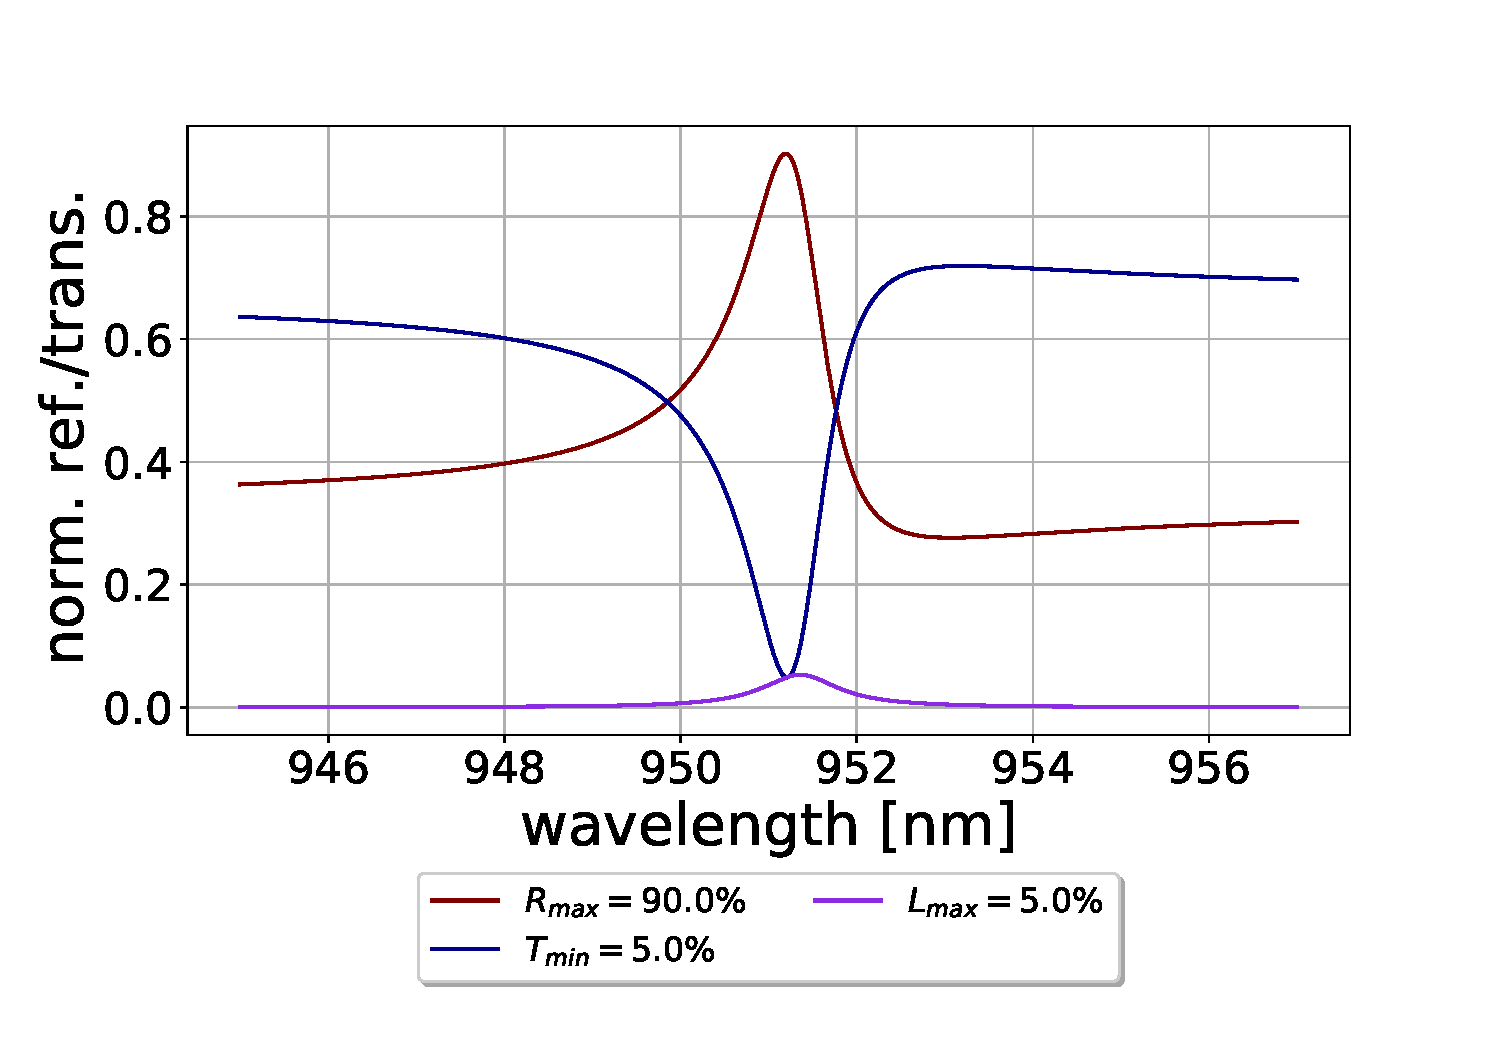
\includegraphics[width=0.7\textwidth]{figures/arbitrary_lossy_grating_ref_trans.pdf}
    \caption{Simulated reflectiviy and transmission spectra of a grating of parameters given in eq. (\ref{eq:optical_grating_params}) with a synthetically added non-zero resonant loss term. The purple line indicate the corresponding grating losses.}
    \label{fig:lossy_grating_spectrum}
\end{figure}

\subsection{The single Fano cavity}

\subsubsection{The single Fano cavity model}

The single Fano cavity consists of a planar broadband mirror, and a sub-wavelength grating, i.e. a Fano mirror, as described in section \ref{sec:fano_mirror} and seen in figure \ref{fig:broadband_and_single_fano_sketch} where schematics of the single Fano and broadband cavity configurations are shown. While the broadband mirror has fixed optical properties, the Fano mirror has transmission and reflection coefficients dependent on the incident wavelength, according to solutions to the coupled differential equations of eq. (\ref{eq:lossy couples diff. eqs.}). 

\begin{figure}[h!]
    \centering
    \begin{subfigure}[b]{0.3\textwidth}
        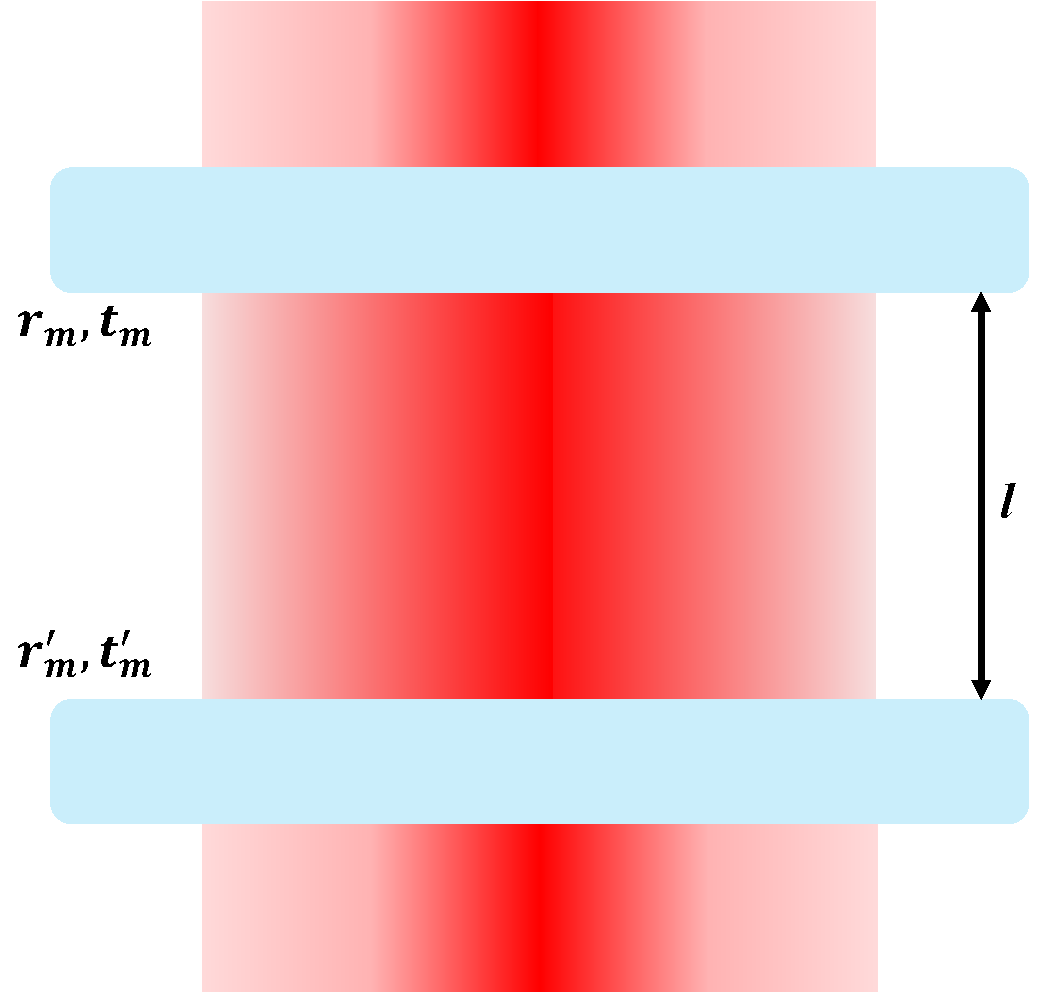
\includegraphics[width=\textwidth]{figures/broadband_sketch.pdf}
        \caption{}
        \label{fig:broadband_sketch}
    \end{subfigure}
    \hspace{1cm}
    \begin{subfigure}[b]{0.3\textwidth}
        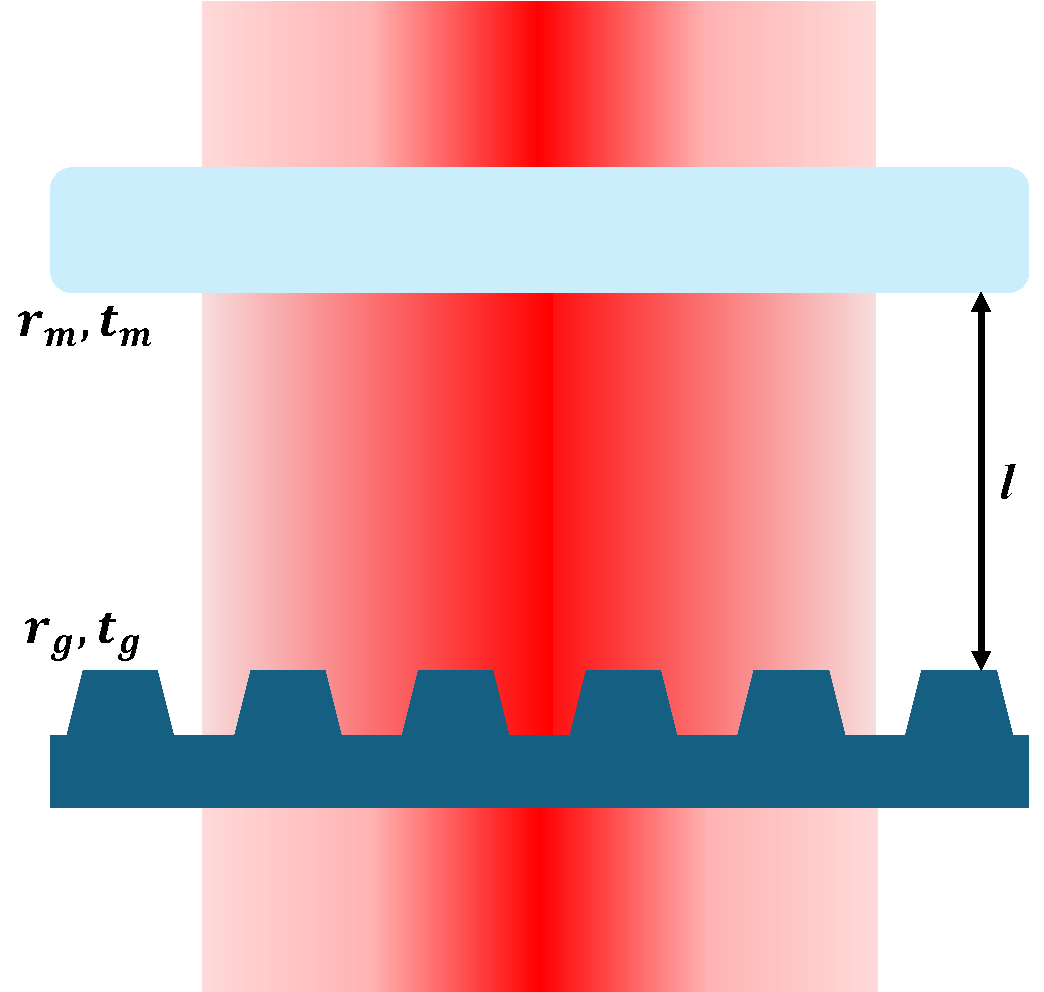
\includegraphics[width=\textwidth]{figures/single_fano_sketch.pdf}
        \caption{}
        \label{fig:single_fano_sketch}
    \end{subfigure}
    \caption{In (a) is seen the schematics of a cavity consisting of two broadband mirrors with transmission and reflectivity coefficients $t_m$, $r_m$, $t_m^{\prime}$, and $r_m^{\prime}$. (b) shows the schematics of a single Fano cavity consisting of one broadband mirror with coefficients $t_m$, $r_m$ and one Fano mirror with wavelength dependent coefficients $t_g$, $r_g$. The reflectors in either cavity are separated by a cavity length $l$.}
    \label{fig:broadband_and_single_fano_sketch}
\end{figure}

In order to model the single Fano cavity transmission spectra, we therefore consider the transmission function of a normal incident and planer Fabry-Perot cavity in eq. (\ref{eq:fabry_perot_trans}) with $r,t \rightarrow r_m,t_m$ and $r^{\prime},t^{\prime} \rightarrow r_g(\lambda),t_g(\lambda)$\cite{Naesby}. Here the subscript $m$ indicates the broadband \emph{mirror} coefficients, and $g$ is for \emph{grating}, which indicates the coefficients of the Fano mirror. Rewriting eq. (\ref{eq:fabry_perot_trans}) such that it describes the normalized transmission amplitude, through the single Fano cavity, $T_{cav} = |E_{out}|^2/|E_{0,in}|^2$ we get
\begin{equation}
    T_{cav} = \left|\frac{t_m t_g(\lambda) e^{i\phi}}{1 - r_m r_g e^{2i\phi}}\right|^2,
    \label{eq:single_fano_trans}
\end{equation}
where $\phi = 2\delta = kl$, $k=2 \pi / \lambda$ and $l$ is the cavity length, as is consistent with the general case described in section \ref{sec:fano_mirror}.

\subsubsection{Transmission linewidth}\label{sec:single_fano_cavity_trans_linewidth}

We aim to analytically describe how the transmission spectrum at, or close to, the overall resonance behaves as a function of the incident wavelength. The overall resonance is the term used for the case of $\lambda_g \approx \lambda_c \approx \lambda_l$, where $g,c,l$ stands for grating/guided-mode, cavity and laser, respectively, and the Fano model is hence generalized for this specific scenario. Considering the case where the cavity resonance closely resembles the guided-mode resonance of the Fano mirror (the zero-transmission wavelength), eq. (\ref{eq:single_fano_trans}) can be approximated well by
\begin{equation}
    T_{cav} \approx \frac{A}{1 + \left( \frac{\Delta}{1 - \nu \Delta} \right)^2},
    \label{eq:general_fano_model}
\end{equation}
where $\Delta = (\lambda - \lambda_c) / \delta \lambda$ is the detuning from the cavity resonance normalized by the HWHM $\delta \lambda$, and $\nu$ is a constant describing the asymmetry of the single Fano transmission spectrum. \cite{Mitra}\cite{Darki} 

From eq. (\ref{eq:general_fano_model}) it can be shown that the HWHM of the Fano transmission profile around the overall resonance wavelength, i.e. when $\lambda_c \approx \lambda_0$, is approximately given as
\begin{equation}
    \delta \lambda \approx \frac{1}{\frac{1}{\delta \lambda_c} + \frac{1}{\delta \lambda_g}},
    \label{eq:analytical_linewidth}
\end{equation}
where 
\begin{equation}
    \delta \lambda_c = \frac{\lambda_0^2}{8 \pi l} (|t_g(\lambda_0)|^2 + |t_m|^2 + L)
    \label{eq:analytical_linewidth_broadband}
\end{equation}
is the HWHM of a broadband cavity and
\begin{equation}
    \delta \lambda_g = \frac{\gamma_{\lambda}}{2 (1-r_d)}(|t_g(\lambda_0)|^2 + |t_m|^2 + L)
    \label{eq:analytical_linewidth_single_fano}
\end{equation}
is the HWHM of the Fano cavity in the so-called Fano regime.\cite{Mitra}\cite{Darki} In eqs. (\ref{eq:analytical_linewidth})-(\ref{eq:analytical_linewidth_single_fano}) $\lambda_0$ is the Fano cavity resonance wavelength, $l$ is the cavity length, $L = \left(1 - |r_g(\lambda_0)|^2 - |t_g(\lambda_0)|^2\right)$ is the total additional losses of the cavity when on resonance, $\gamma \lambda$ is the width of the guided-mode resonance of the Fano mirror and $r_d$ is the off-resonance, or \emph{direct}, reflectivity of the Fano mirror.

The \emph{Fano regime} and its counterpart the so-called \emph{standard regime} are defined for a given single Fano cavity, by its length $l$. By inspection of eqs. (\ref{eq:analytical_linewidth_broadband}) and (\ref{eq:analytical_linewidth_single_fano}) it is seen that for $l \rightarrow \infty$ the linewidth in eq. (\ref{eq:analytical_linewidth}) is dominated by the broadband cavity term, while for the opposite case, $l \rightarrow 0$, the linewidth is predominantly given by the Fano cavity term. 

Generally the Fano regime describes the cavity lengths for which eq. (\ref{eq:analytical_linewidth}) shows a significant divergence from the broadband linewidth in eq. (\ref{eq:analytical_linewidth_broadband}). Oppositely, when in the standard regime the broadband and Fano cavity produces resonance transmission peaks of comparable, if not equal, linewidths.

We now introduce a single Fano cavity consisting of the Fano mirror introduced in section \ref{sec:fano_mirror} and sketched in figure \ref{fig:MIST_grating_sketch}, and a broadband mirror of reflectivity $|r|^2=90\%$ and transmission $|t|^2=1\%$. Figures \ref{fig:standard_regime_trans} and \ref{fig:fano_regime_trans} depicts examples of the transmission spectra in the standard and Fano regimes together with their respective complimentary broadband cavity transmission profiles. The reflectiviy amplitude of the Fano mirror is shown in both figures.

\begin{figure}[h!]
    \centering
    \begin{subfigure}[b]{0.49\textwidth}
        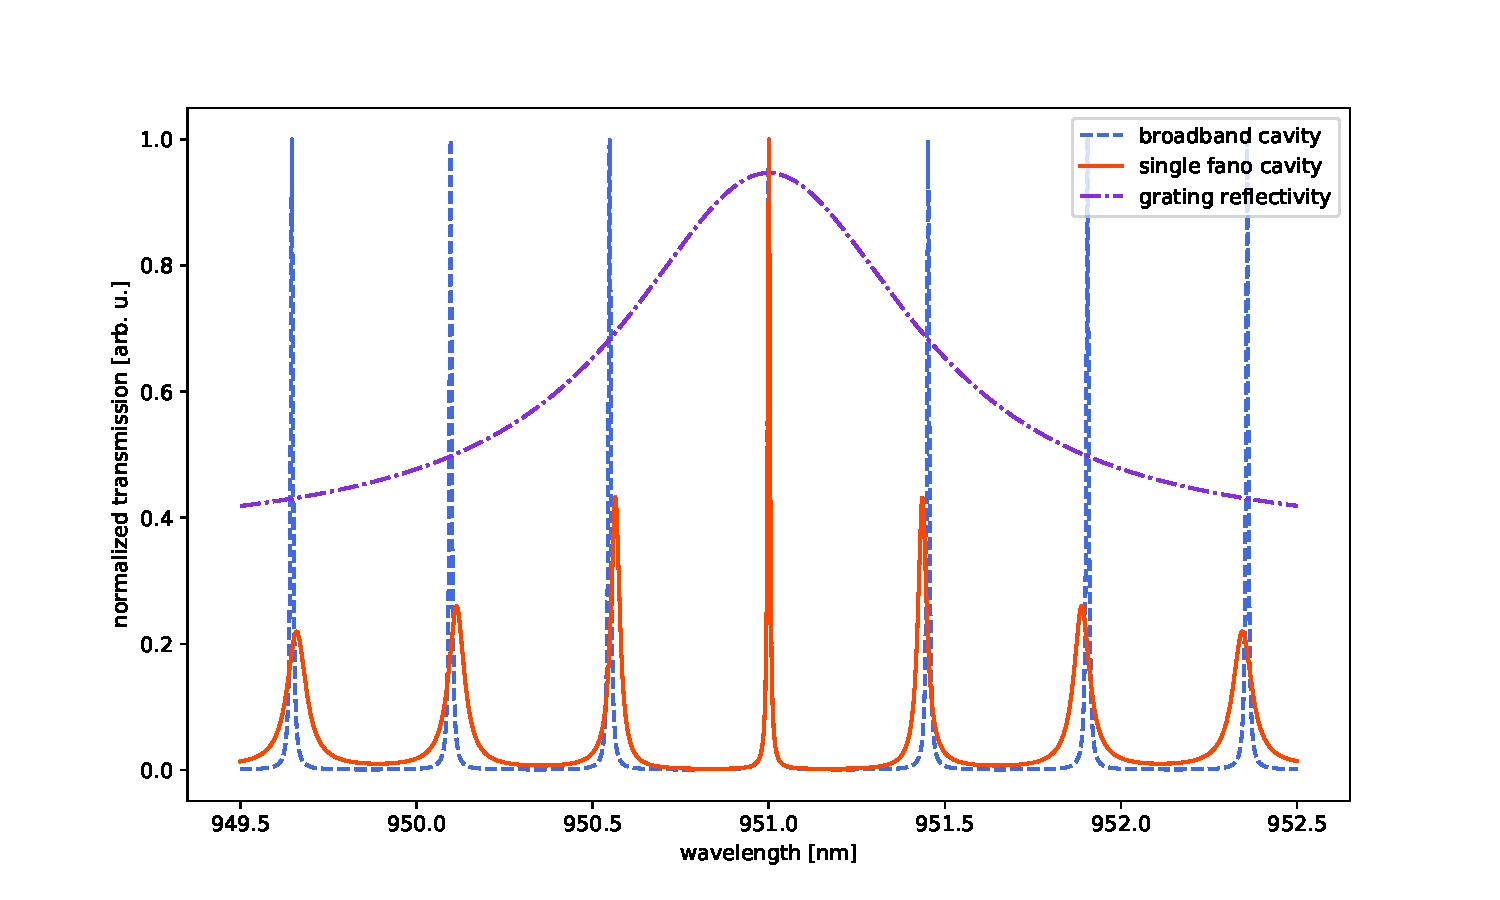
\includegraphics[width=\textwidth]{figures/fano_and_broadband_cavity_1000um.pdf}
        \caption{}
        \label{fig:standard_regime_trans}
    \end{subfigure}
    \begin{subfigure}[b]{0.49\textwidth}
        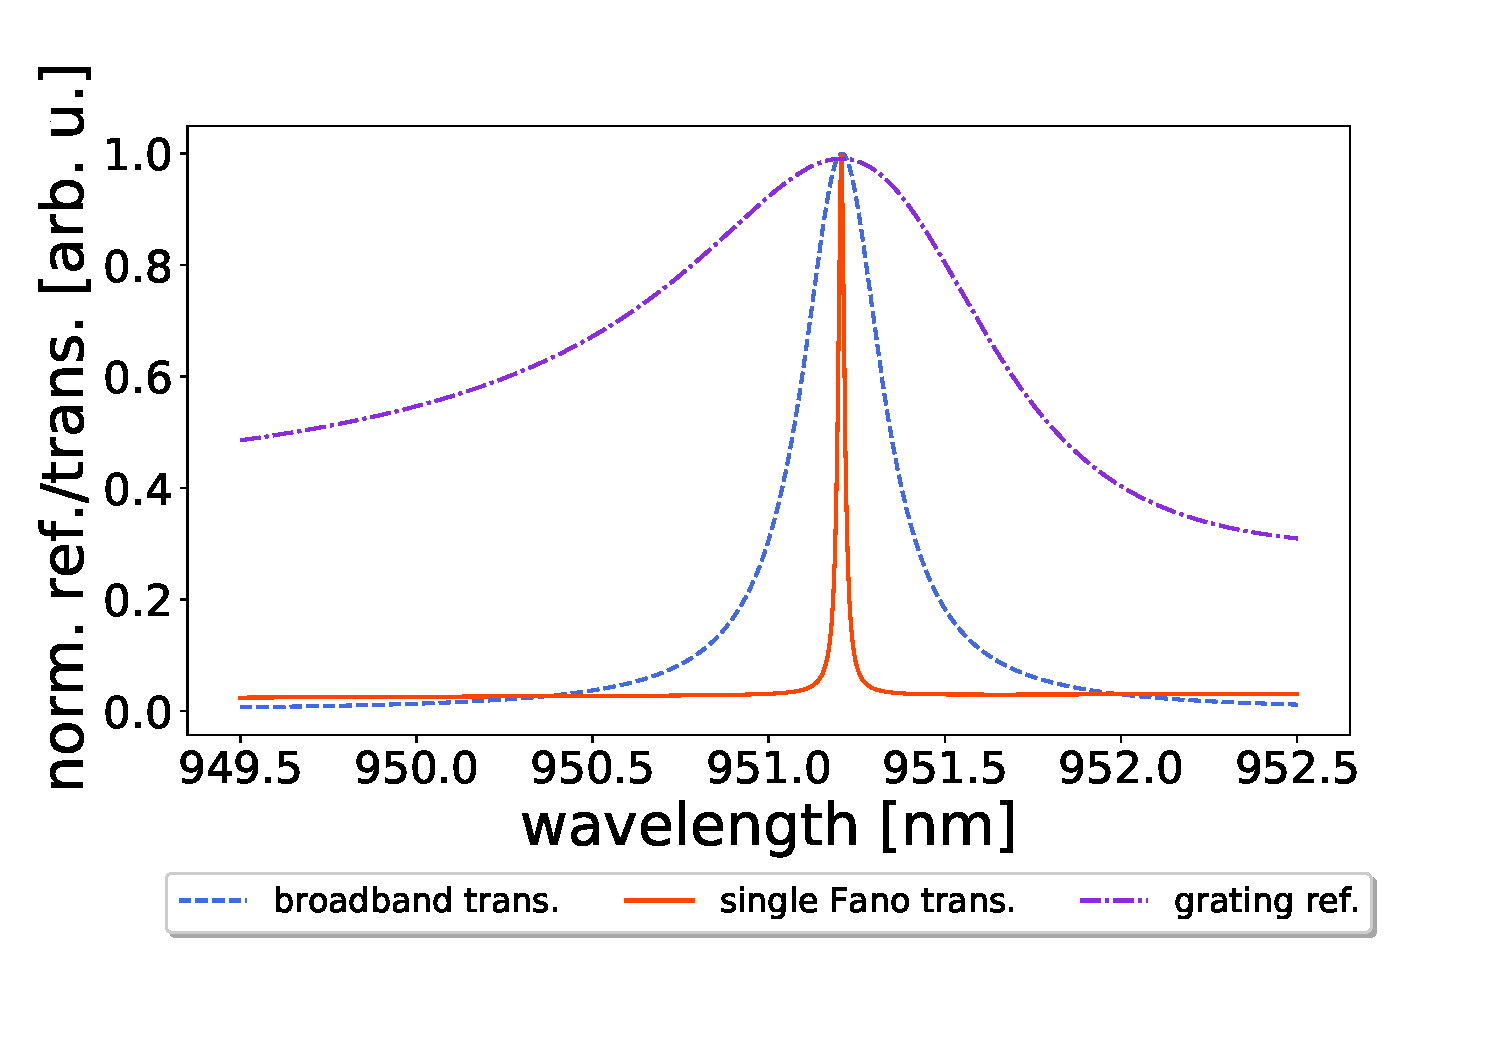
\includegraphics[width=\textwidth]{figures/fano_and_broadband_cavity_5um.pdf}
        \caption{}
        \label{fig:fano_regime_trans}
    \end{subfigure}
    \caption{In (a) is seen the comparison of broadband and single Fano cavity transmission spectra for a cavity length of $l \approx 1000 \mu m$, i.e. in the \emph{standard} regime. (b) shows the same comparison, but for a cavity length of $l \approx 5 \mu m$, i.e. in the so-called \emph{Fano} regime.}
\end{figure}

Figure \ref{fig:standard_regime_trans} shows the transmission spectra of the two cavities for a length of $l \approx 1000\mu m$, i.e. in the standard regime. It is clear from inspection of the figure that the resonance transmission profile of the standard broadband cavity is not wavelength dependent, in the sense that all fringes appear to have the same high finesse $\mathcal{F}$, i.e. ratio between the FSR and HWHM. This is not the case for the Fano cavity which is due to the wavelength dependence of the optical properties of the Fano mirror, as this causes the transmission and reflectivity to \emph{only} match those of the broadband mirror when on resonance. Furthermore, no significant difference in linewidth is seen for the transmission of the two cavities on resonance, as predicted by eq. (\ref{eq:analytical_linewidth}).

In figure \ref{fig:fano_regime_trans}, the transmission spectra of both cavities are shown for a length of $l\approx 5 \mu m$, i.e. in the Fano regime. Here it is clearly seen that while the standard cavity, as expected, experiences broadening for shorter cavity lengths, this is not the case for the Fano cavity transmission peak.

\begin{figure}[h!]
    \centering
    \begin{subfigure}[c]{0.7\textwidth}
        \centering
        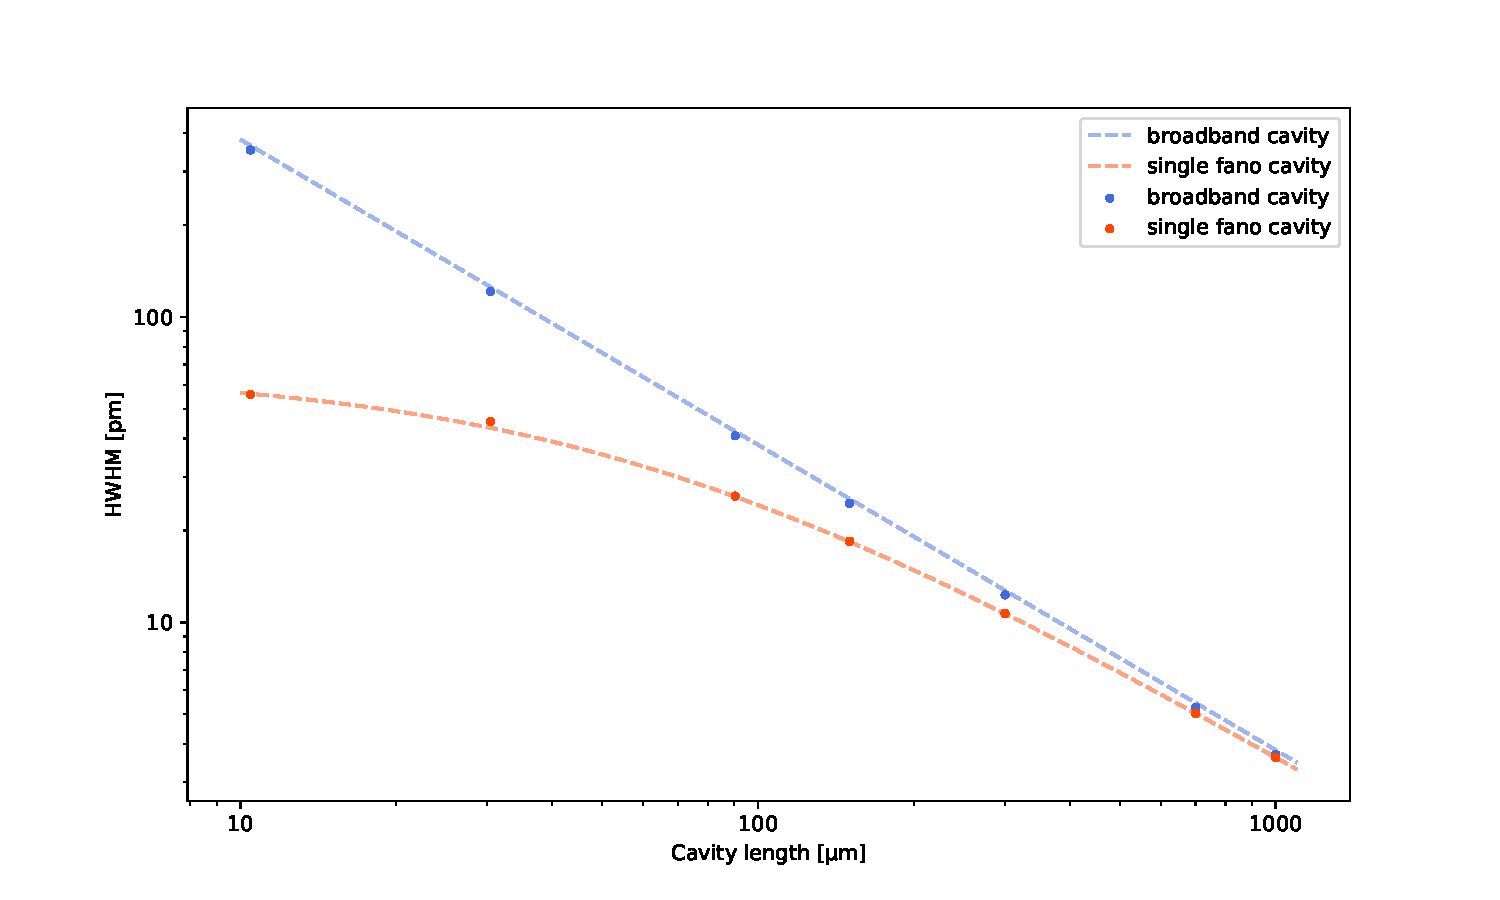
\includegraphics[width=\textwidth]{figures/HWHM_broadband_vs_single_sim.pdf}
        \caption{}
        \label{fig:HWHM_broadband_vs_single_fano}
    \end{subfigure}
    \begin{subfigure}[c]{0.49\textwidth}
        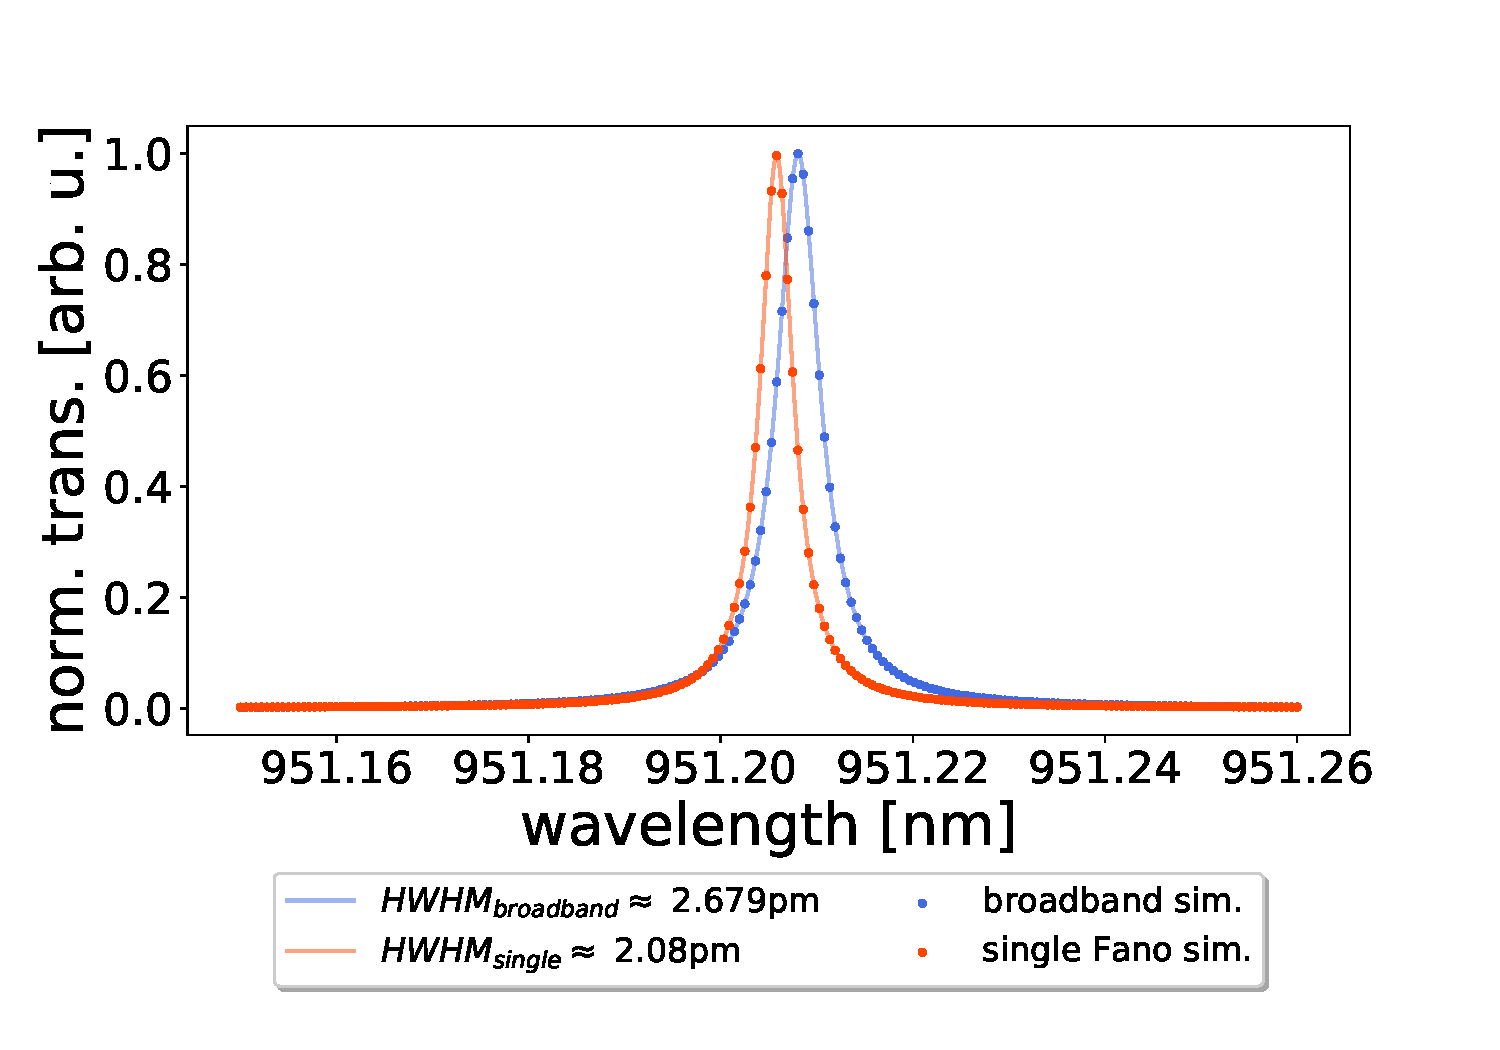
\includegraphics[width=\textwidth]{figures/sim_single_vs_broadband_270um.pdf}
        \caption{}
        \label{fig:270um_broadband_and_single_fano_peak}
    \end{subfigure}
    \begin{subfigure}[c]{0.49\textwidth}
        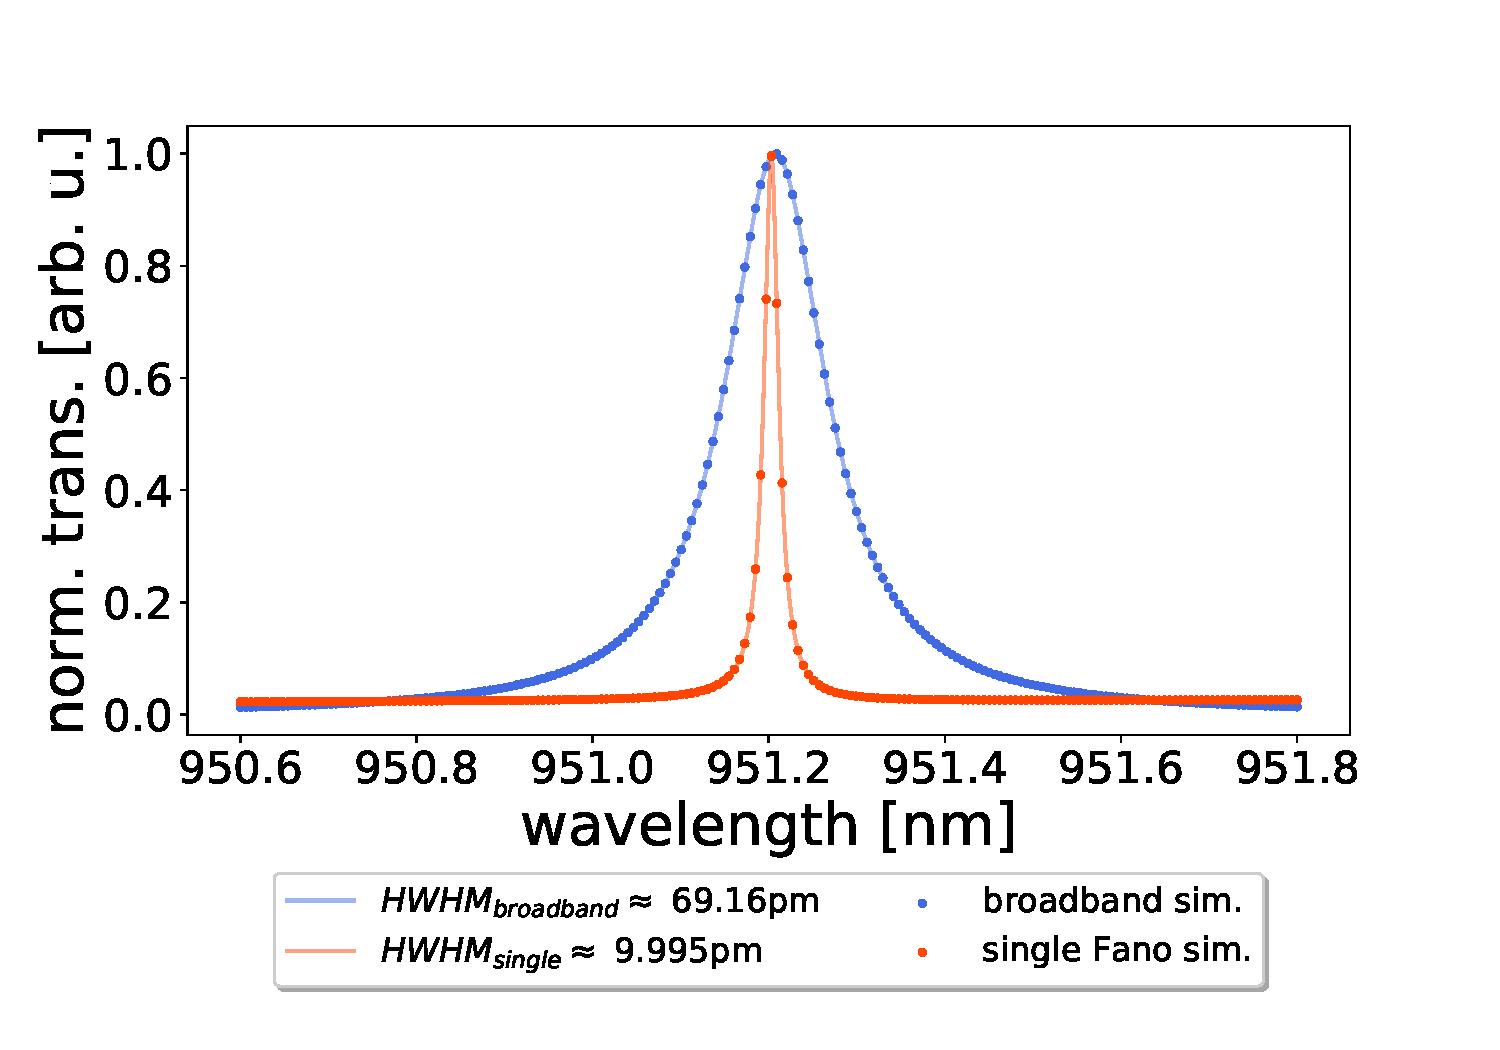
\includegraphics[width=\textwidth]{figures/sim_single_vs_broadband_10um.pdf}
        \caption{}
        \label{fig:10um_broadband_and_single_fano_peak}
    \end{subfigure}
    \caption{(a) shows the approximate analytical resonance linewidths (eq. (\ref{eq:analytical_linewidth})) as a function of cavity length for the broadband and single Fano cavities together with linewidths of transmission profiles simulated using eq. (\ref{eq:single_fano_trans}) and eq. (\ref{eq:fabry_perot_trans}), found as parameters of least squares fits, for comparison. In (b) and (c) is seen transmission spectra of broadband and single Fano cavities of lengths $\sim 270 \mu m$ and $\sim 10 \mu m$, respectively. The spectra shown indicate each their respective linewidths, and are examples of the values plotted in (a).}
\end{figure}

Figure \ref{fig:HWHM_broadband_vs_single_fano} models the behavior of the linewidth of the single Fano cavity compared with the one for a broadband cavity of similar optical properties, as a function of wavelength. Here it is easily seen where the linewidth of the single Fano transmission begins to saturate, and hence deviate from the one of the broadband cavity. The plotted line in the figure is calculated using eq. (\ref{eq:analytical_linewidth}) while the points depicit linewidths found as a fitting parameter from a least squares fit of the general Fano model in eq. (\ref{eq:general_fano_model}) to transmission spectra simulated by the Fabry-Perot (eq. (\ref{eq:fabry_perot_trans})) and single Fano (eq. (\ref{eq:single_fano_trans})) transmission functions. Finally, it can be concluded that the approximate analytical expression for the linewidth of the broadband and single fano cavities in eq. (\ref{eq:analytical_linewidth}) correlates very well with the values found from the simulated spectra.

\subsection{The double Fano cavity}

\subsubsection{The double Fano cavity model}

While the single Fano cavity is usually known in the appropriate litterature as simply a \emph{Fano cavity}, I have insisted on including the fact that it contains only one Fano mirror, and hence denoted it the \emph{single} Fano cavity. This addition is justified by the contents of this section, and namely that we now move on to the \emph{double} Fano cavity, which as the name suggests consists of two Fano mirrors. The schematics of this configuration is shown together with the one for the single Fano cavity in figure \ref{fig:single_and_double_fano_sketch}.

\begin{figure}[h!]
    \centering
    \begin{subfigure}[b]{0.3\textwidth}
        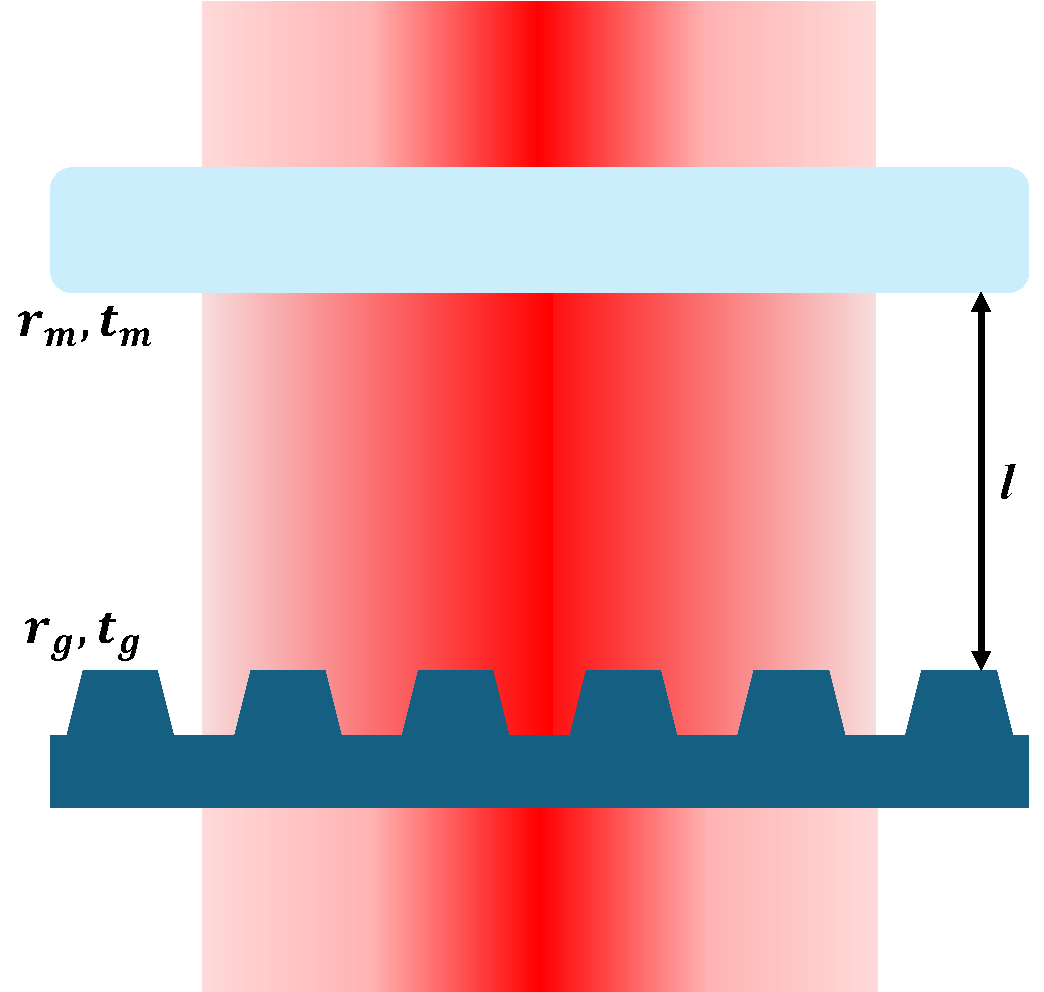
\includegraphics[width=\textwidth]{figures/single_fano_sketch.pdf}
        \caption{}
        \label{fig:single_fano_sketch2}
    \end{subfigure}
    \hspace{1cm}
    \begin{subfigure}[b]{0.3\textwidth}
        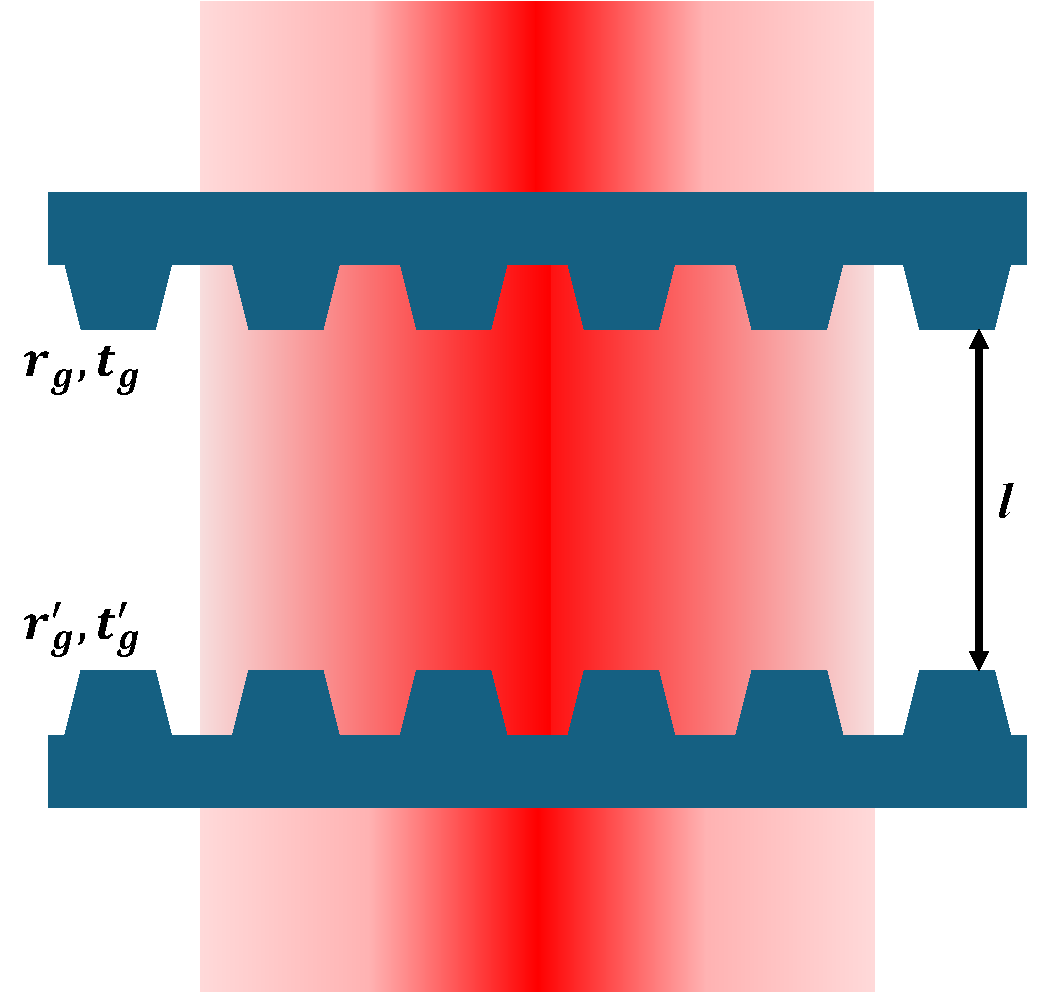
\includegraphics[width=\textwidth]{figures/double_fano_sketch.pdf}
        \caption{}
        \label{fig:double_fano_sketch}
    \end{subfigure}
    \caption{(a) shows schematics of the single Fano cavity consisting of a broadband mirror with transmission and reflectivity coefficients $t_m$, $r_m$ and a Fano mirror with coefficients $t_g$, $r_g$. (b) shows the schematics of the double Fano cavity consisting of two Fano mirrors with coefficients $t_g$, $r_g$, $t_g^{\prime}$, $r_g^{\prime}$. Both cavities are separated by a cavity length $l$.}
    \label{fig:single_and_double_fano_sketch}
\end{figure}

Here it is evident that instead of having one set of reflectivity and transmission coefficients that depend on the incident wavelength, we now have two. In order to model the transmission of the double Fano cavity, we once again consider the transmission function for the normal incident and planar Fabry-Perot cavity in eq. (\ref{eq:fabry_perot_trans}), this time with $r,t \rightarrow r_g(\lambda),t_g(\lambda)$ and $r^{\prime},t^{\prime} \rightarrow r_g^{\prime}(\lambda),t_g^{\prime}(\lambda)$\cite{Naesby}. We rewrite the Fabry-Perot transmission function with the addressed substitutions of the optical coefficients and such that it decribes the normalized transmission amplitudes $T_{cav} = |E_{out}|^2/|E_{0,in}|^2$ and get
\begin{equation}
    T_{cav} = \frac{t_g(\lambda) t_g^{\prime}(\lambda) e^{i\phi}}{1 - r_g(\lambda)r_g^{\prime}(\lambda) e^{2 i \phi}}.
    \label{eq:double_fano_transmission}
\end{equation}
The subscript $g$ indicates a grating transmission or reflectivity.

We now introduce a double Fano cavity consisting of two identical Fano mirrors, each as sketched in figure \ref{fig:MIST_grating_sketch} in section \ref{sec:fano_mirror}, and thus with optical parameters given in eq. (\ref{eq:optical_grating_params}). Figure \ref{fig:double_fano_transmission} shows an example of the normalized transmission spectrum of this double Fano cavity on- and off-resonance for a cavity length of $l \approx 30 \mu m$. The spectrum was found using eq. (\ref{eq:double_fano_transmission}).

\begin{figure}[h!]
    \centering
    \begin{subfigure}[c]{0.49\textwidth}
        \centering
        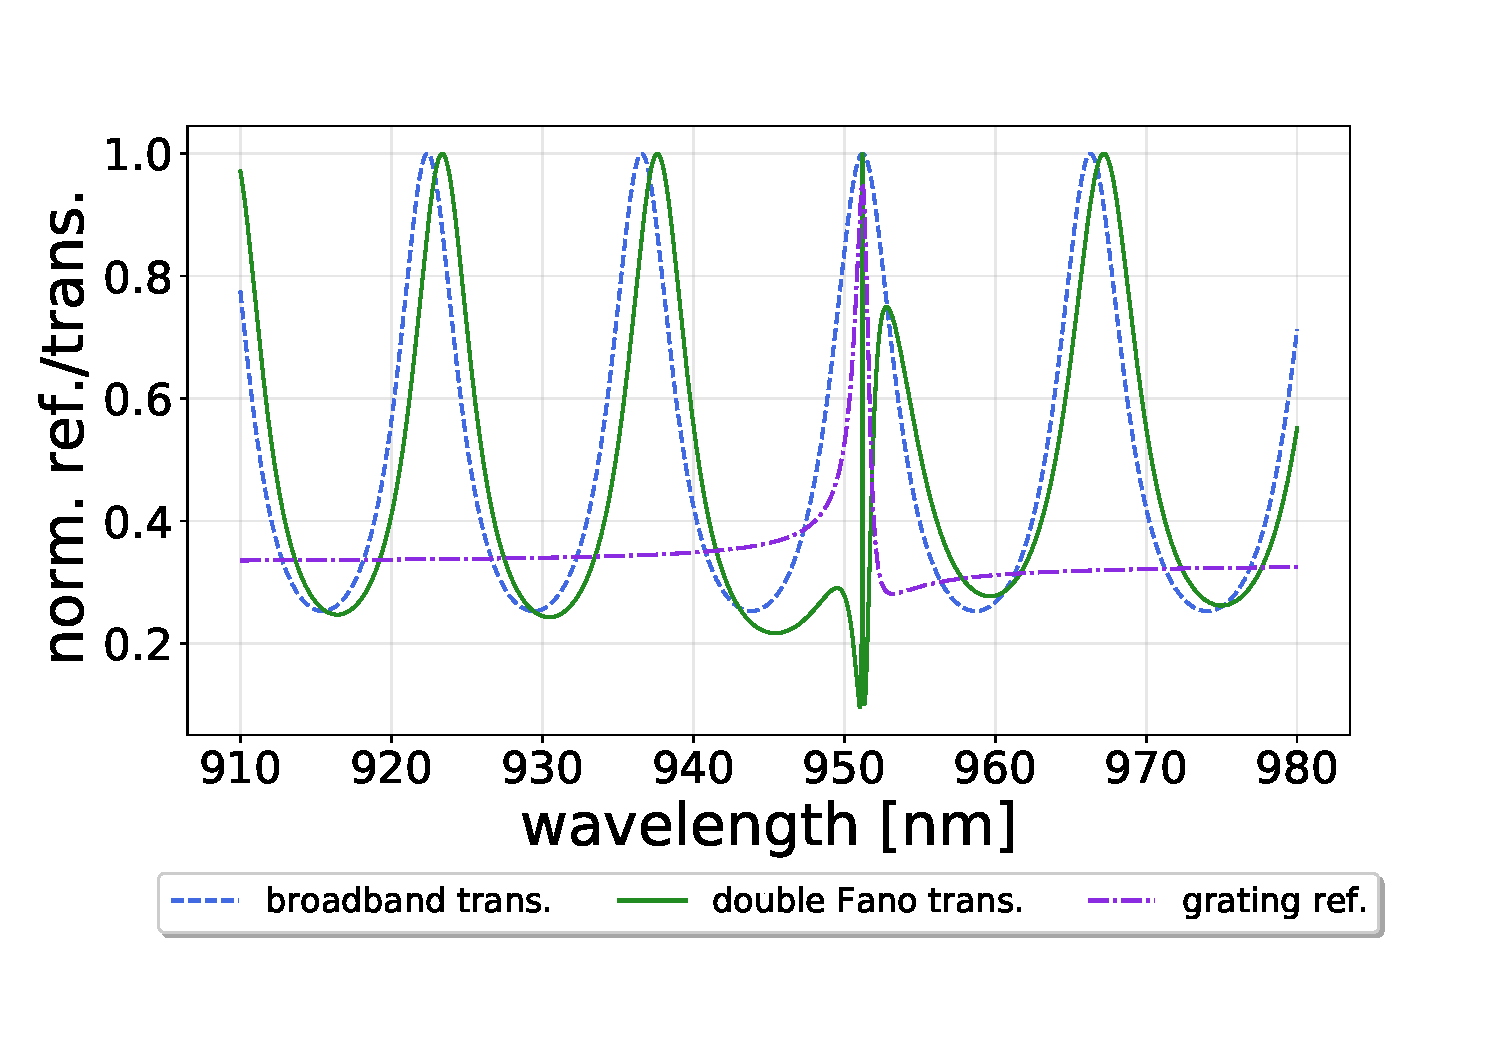
\includegraphics[width=\textwidth]{figures/double_fano_full_range_30um.pdf}
        \caption{}
        \label{fig:double_full_range}
    \end{subfigure}
    \begin{subfigure}[c]{0.49\textwidth}
        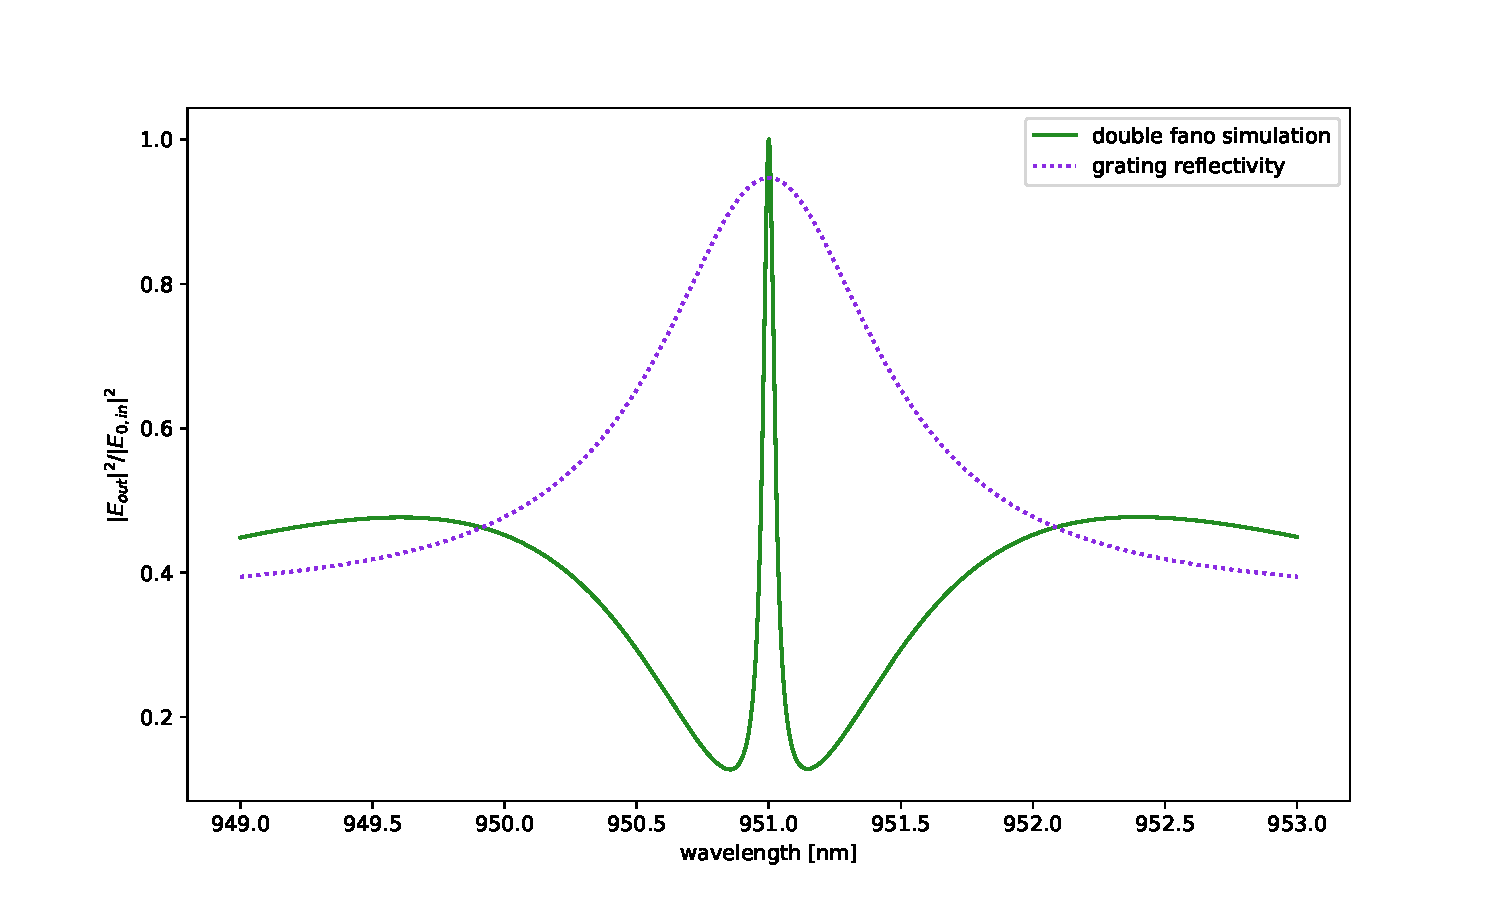
\includegraphics[width=\textwidth]{figures/double_fano_short_range_30um.pdf}
        \caption{}
        \label{fig:double_short_range}
    \end{subfigure}
    \caption{An example of a normalized double Fano transmission spectrum of a cavity of length $l \approx 30 \mu m$. (a) shows a long-range wavelength scan, depicting both the on- and off-resonance behaviour of the double Fano cavity transmission. Note that the broadband cavity transmission for a cavity of optical properties given by the direct reflectivity $r_d$ and direct transmission $t_d$ of the Fano mirror is shown. It is readily seen that the resonance peak is placed on a "background" consisting of this function, displaced by a small phase. (b) shows the transmission focussed specifically around the resonance wavelength. Both examples are shown together with the reflectivity of the Fano mirror used to model them.}
    \label{fig:double_fano_transmission}
\end{figure}

\subsubsection{Transmission linewidth}\label{sec:double_fano_lw_theory}

In order to describe the analytical linewidth of the transmisison profile of the double Fano cavity, we take a similar approach as in the single Fano case outlined in section \ref{sec:single_fano_cavity_trans_linewidth}. It can be shown from eq. (\ref{eq:analytical_linewidth}) when including the wavelength dependence of the optical coefficients of both Fano mirrors, that the HWHM $\delta \lambda$ of the double Fano cavity transmission profile is approximately given as
\begin{equation}
    \delta \lambda^{double} \approx \frac{1}{\frac{1}{\delta \lambda_c} + \frac{1}{\delta \lambda_g^{double}}},
    \label{eq:analytical_linewidth_double}
\end{equation}
where 
\begin{equation}
    \delta \lambda_c = \frac{\lambda_0^2}{8 \pi l} (|t_g(\lambda_0)|^2 + |t_g^{\prime}(\lambda_0)|^2 + L)
\end{equation}
is still the HWHM of a broadband cavity and
\begin{equation}
    \delta \lambda_g^{double} = \frac{\gamma \lambda}{4 (1-r_d)}(|t_g(\lambda_0)|^2 + |t_g^{\prime}(\lambda_0)|^2 + L).
    \label{eq:double_fano_linewidth_contribution}
\end{equation}
is the HWHM of the double Fano cavity in the Fano regime. Note that $\delta \lambda^{double} = \delta \lambda^{single}/2$ for $l \rightarrow 0$ when eq. (\ref{eq:analytical_linewidth_double}) is predominantly given by eq. (\ref{eq:double_fano_linewidth_contribution}). In this brief evaluation of the estimated analytical linewidth of the double Fano transmission profile it is assumed that all defining parameters of the two Fano mirrors are identical, except for the cavity and guided-mode resonance wavelengths $\lambda_{0,1}$. Namely the following relevant parameters are assumed identical,
\begin{equation}
    r_d = r_d^{\prime} \: \text{ and } \: \gamma \lambda = \gamma \lambda^{\prime}.
\end{equation}
In this way any spectral detuning of the two Fano mirrors used to make a cavity is included in the analytical expression. The spectral detuning, and the effect hereof, will be further described in section \ref{sec:spectral_detuning}.

\subsubsection{Single and double Fano cavity comparison}\label{sec:single_vs_double_comparison_theory}

Using the analytical expression for the double Fano cavity transmission in eq. (\ref{eq:analytical_linewidth_double}) we are now in a position to compare the single and double Fano cavities. Note that we at this point only consider the ideal case of the double Fano cavity where additional cavity losses are neglected and the two Fano mirrors used are identical, i.e. the cavity is said to be \emph{symmetrical}. The additional cavity losses are explicitly set to be given as
\begin{equation}
    L = 1-|r_g|^2-|t_g|^2 = 0.
\end{equation}

\begin{figure}[h!]
    \centering
    \begin{subfigure}[c]{0.49\textwidth}
        \centering
        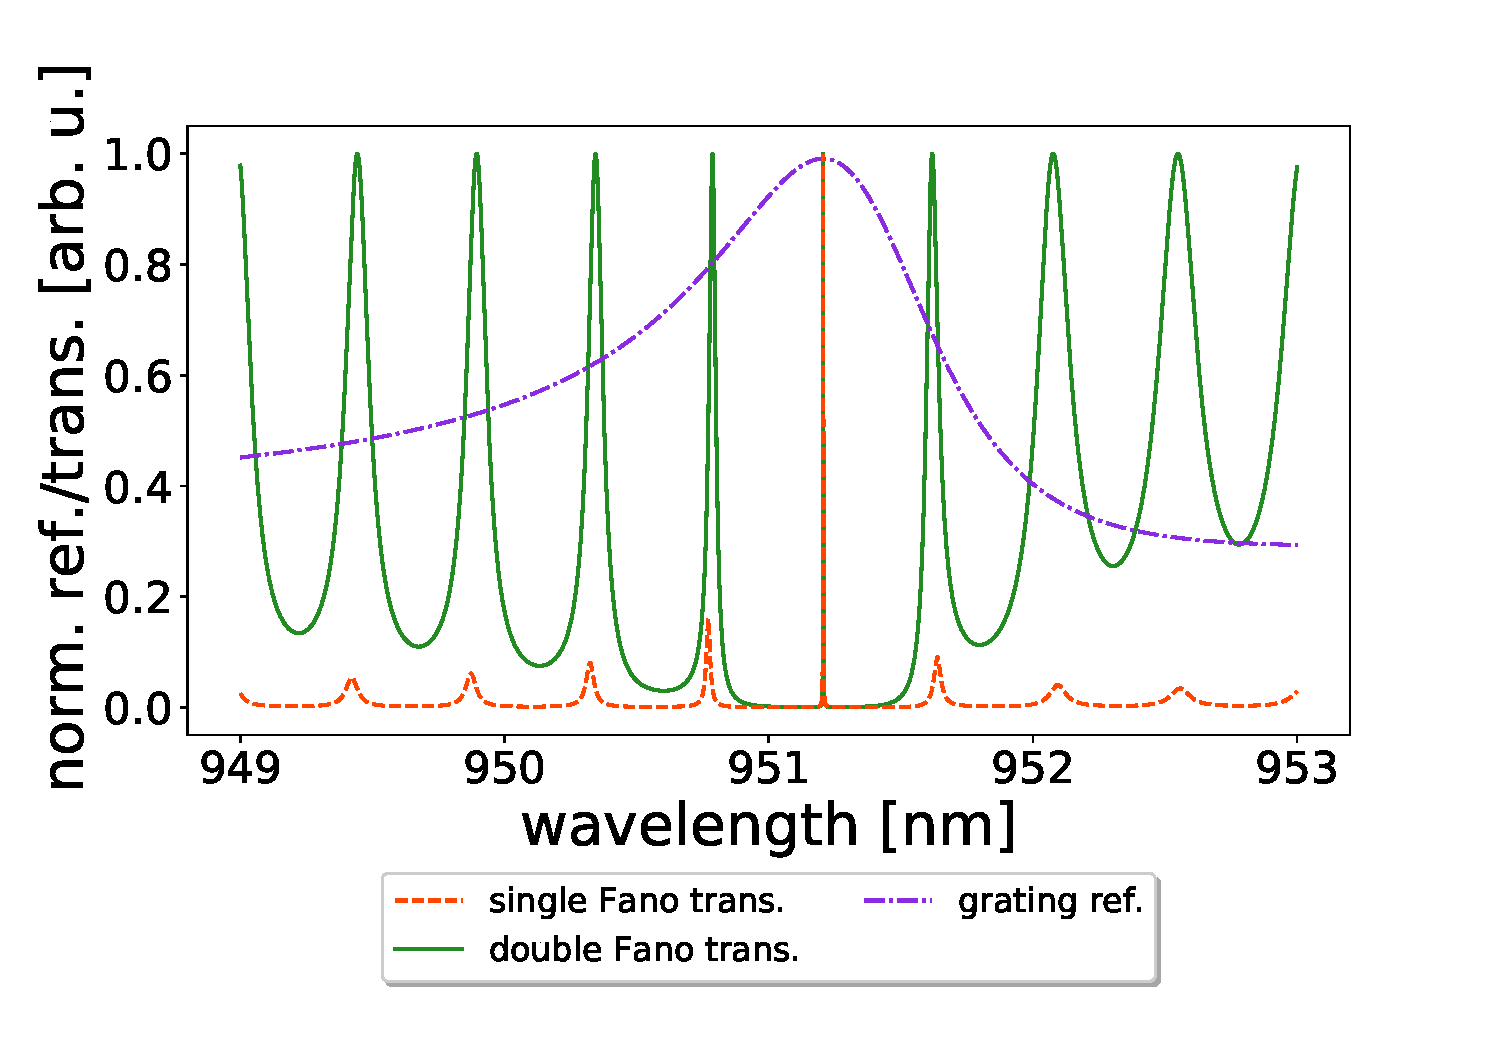
\includegraphics[width=\textwidth]{figures/single_and_double_1000um.pdf}
        \caption{}
        \label{fig:double_in_standard_regime}
    \end{subfigure}
    \begin{subfigure}[c]{0.49\textwidth}
        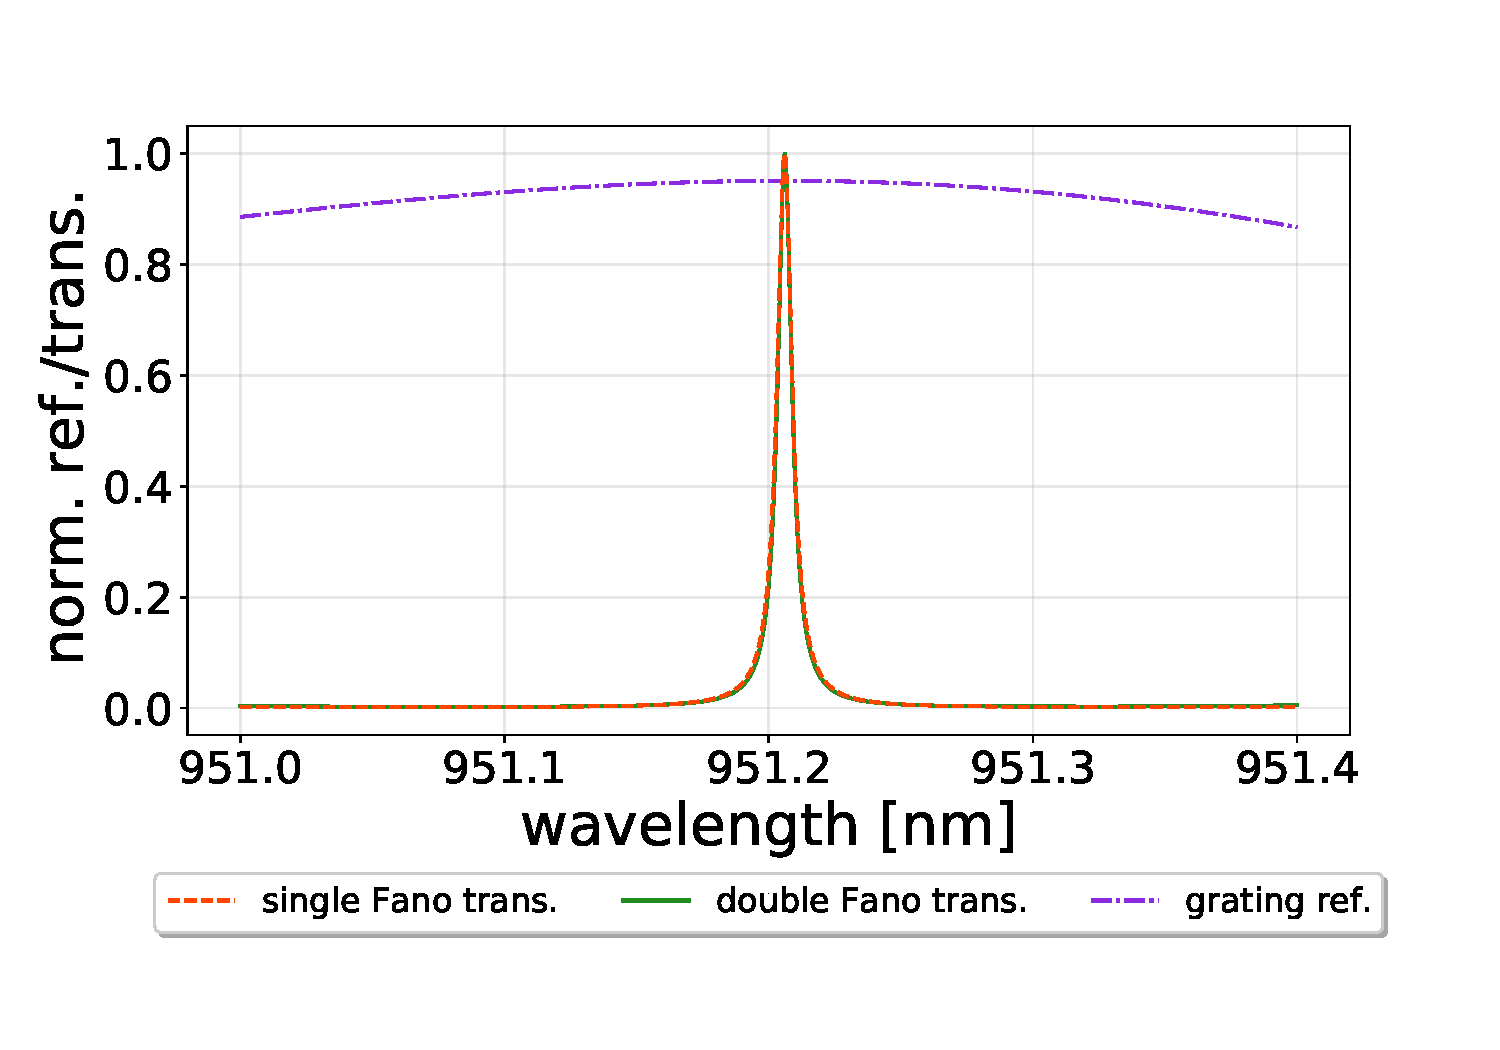
\includegraphics[width=\textwidth]{figures/single_and_double_1000um_zoomed.pdf}
        \caption{}
        \label{fig:double_in_standard_regime_zoomed}
    \end{subfigure}
    \begin{subfigure}[c]{0.49\textwidth}
        \centering
        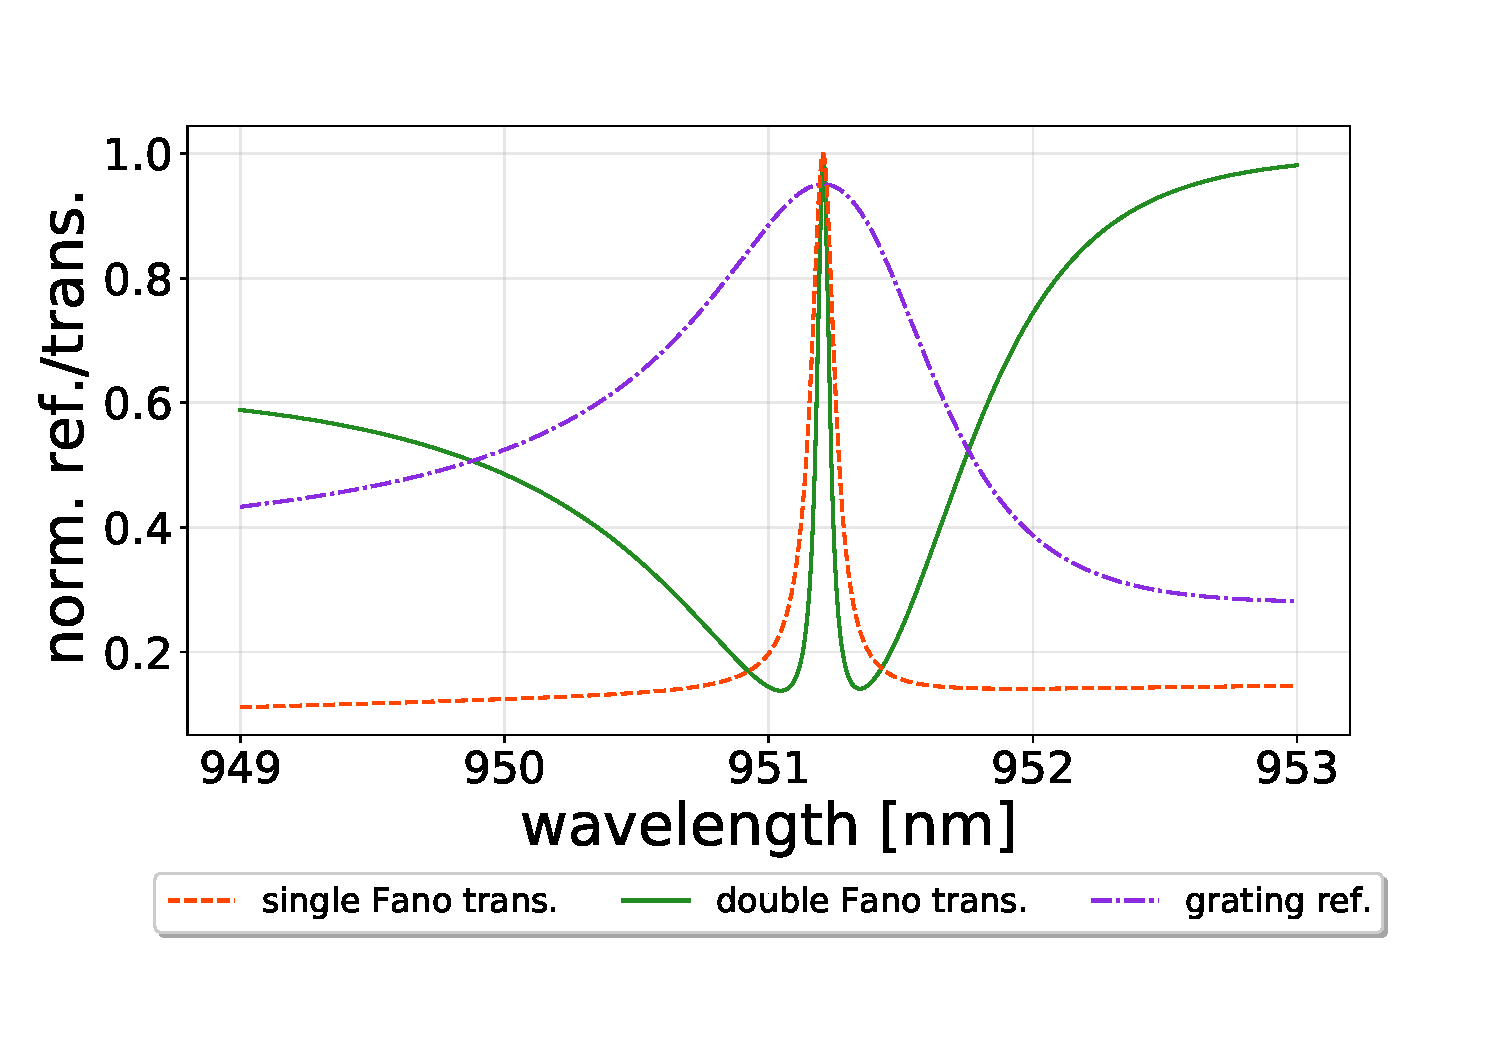
\includegraphics[width=\textwidth]{figures/single_and_double_5um.pdf}
        \caption{}
        \label{fig:double_in_fano_regime}
    \end{subfigure}
    \begin{subfigure}[c]{0.49\textwidth}
        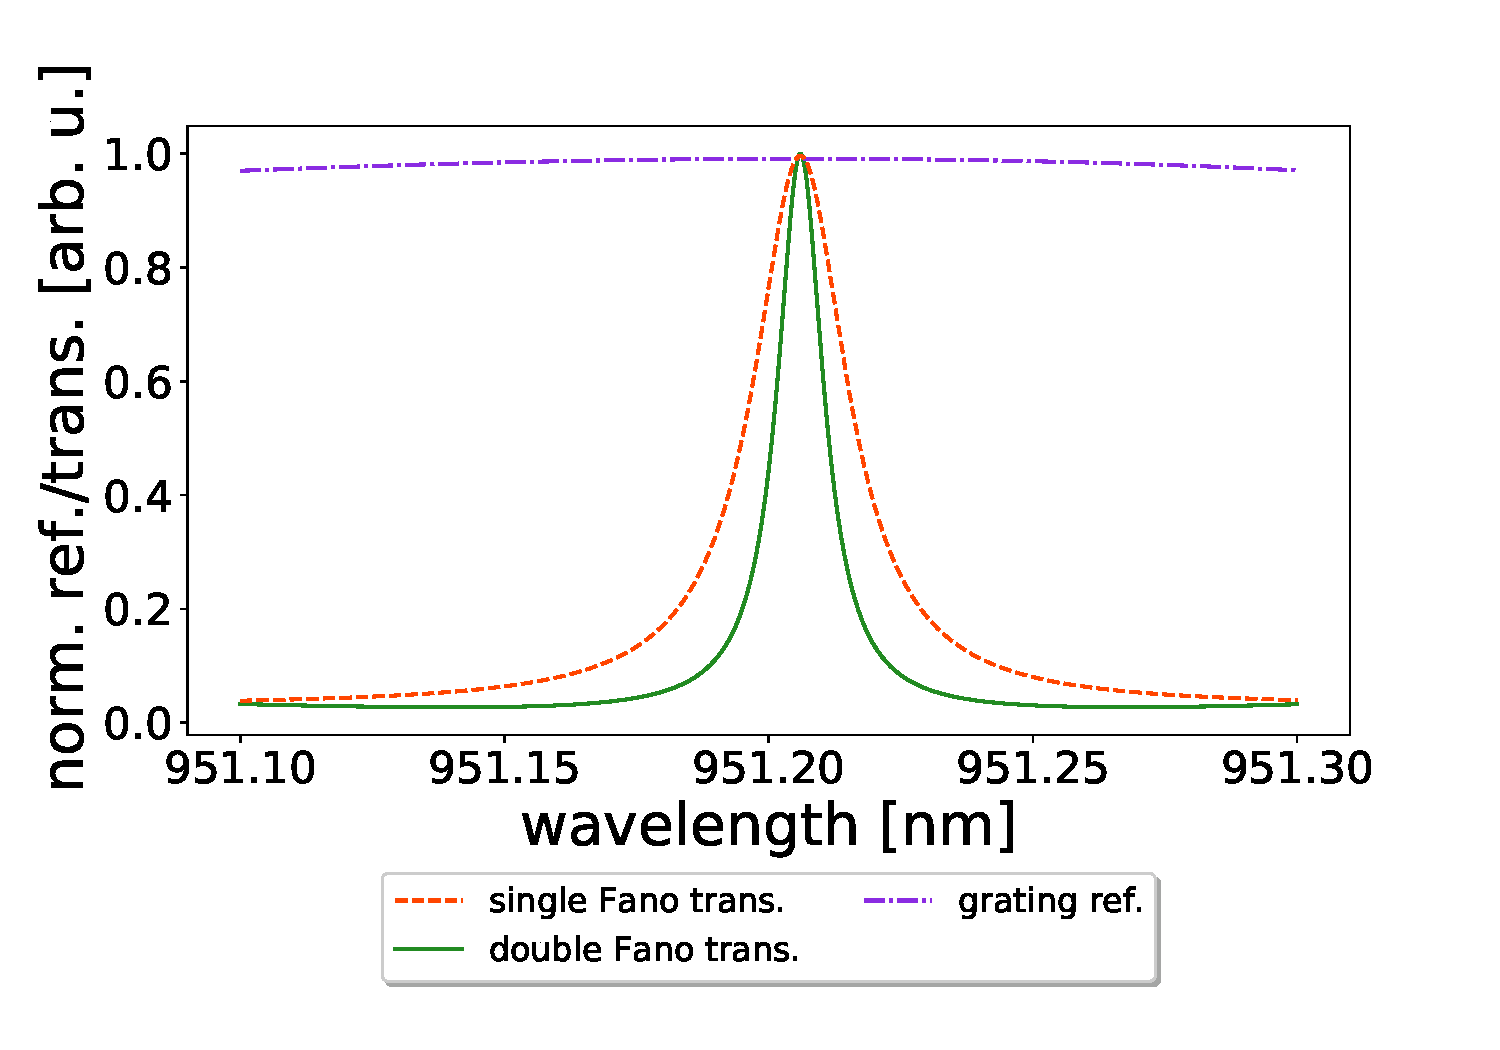
\includegraphics[width=\textwidth]{figures/single_and_double_5um_zoomed.pdf}
        \caption{}
        \label{fig:double_in_fano_regime_zoomed}
    \end{subfigure}
    \caption{Comparison of the single and double Fano transmission spectra in the \emph{standard} and \emph{Fano} regimes. (a) and (b) shows the spectral comparison for a cavity of length $l \approx 1000 \mu m$, i.e. in the \emph{standard} regime, while (c) and (d) shows the same for a cavity of length $l \approx 5 \mu m$, i.e. in the \emph{Fano} regime. (b) and (c) show spectra zoomed around the resonance peak, and the Fano mirror reflectivity is depicted in all figures.}
    \label{fig:double_in_standard_and_fano_regimes}
\end{figure}

Figure \ref{fig:double_in_standard_and_fano_regimes} shows the transmission of the ideal double Fano cavity and the corresponding single Fano cavity for comparison. 

Figures \ref{fig:double_in_standard_regime} and \ref{fig:double_in_standard_regime_zoomed} shows the transmission for a cavity length of $l \approx 1000 \mu m$ which is well-inside the standard regime outlined in section \ref{sec:single_fano_cavity_trans_linewidth}, where the standard, broadband and single Fano cavities produce transmission spectra of roughly identical linewidths. In this regime, due to the $1/l$ proportionality of the FSR, the off-resonance behavior of the double Fano cavity transmission is visible in the range plottet. It is seen, contrary to the single Fano cavity, that the transmission at each cavity resonance reaches a normalized transmission of $|E_{out}|^2/|E_{0,in}|^2=1$. This is due to the fact that the two Fano mirrors, while they have wavelength dependent transmission and reflectivity coefficients, always have identical ones for the ideal case. This maximizes the Fabry-Perot transmission function and ensures unity transmission at any cavity resonance. The minimum level of the cavity changes according to the coefficient of finesse, and thus only the Fano mirror reflectivity, hence the HWHM also changes as we move further from the guided-mode resonance. Both the minimum transmission level and the HWHM converge when moving away from the resonance wavelength, when $r \rightarrow r_d$ becomes constant. 

Figures \ref{fig:double_in_fano_regime} and \ref{fig:double_in_fano_regime_zoomed} shows the transmission of a double Fano cavity of length $l \approx 5 \mu m$, i.e. well within the Fano regime. It is seen that the double Fano cavity transmission produces a resonance peak with a HWHM narrower than the one for the single Fano cavity, as is predicted in eq. (\ref{eq:double_fano_linewidth_contribution}). Furthermore, the immediate off-resonance behavior of the double Fano cavity transmission in the Fano regime, is drastically different than for the single Fano cavity. This is due to the collective higher transmission in this region compared with the single Fano case where the broadband mirror has a constant, and often high, reflectivity and hence a correspondingly low transmission.

\begin{figure}[h!]
    \centering
    \begin{subfigure}[c]{0.7\textwidth}
        \centering
        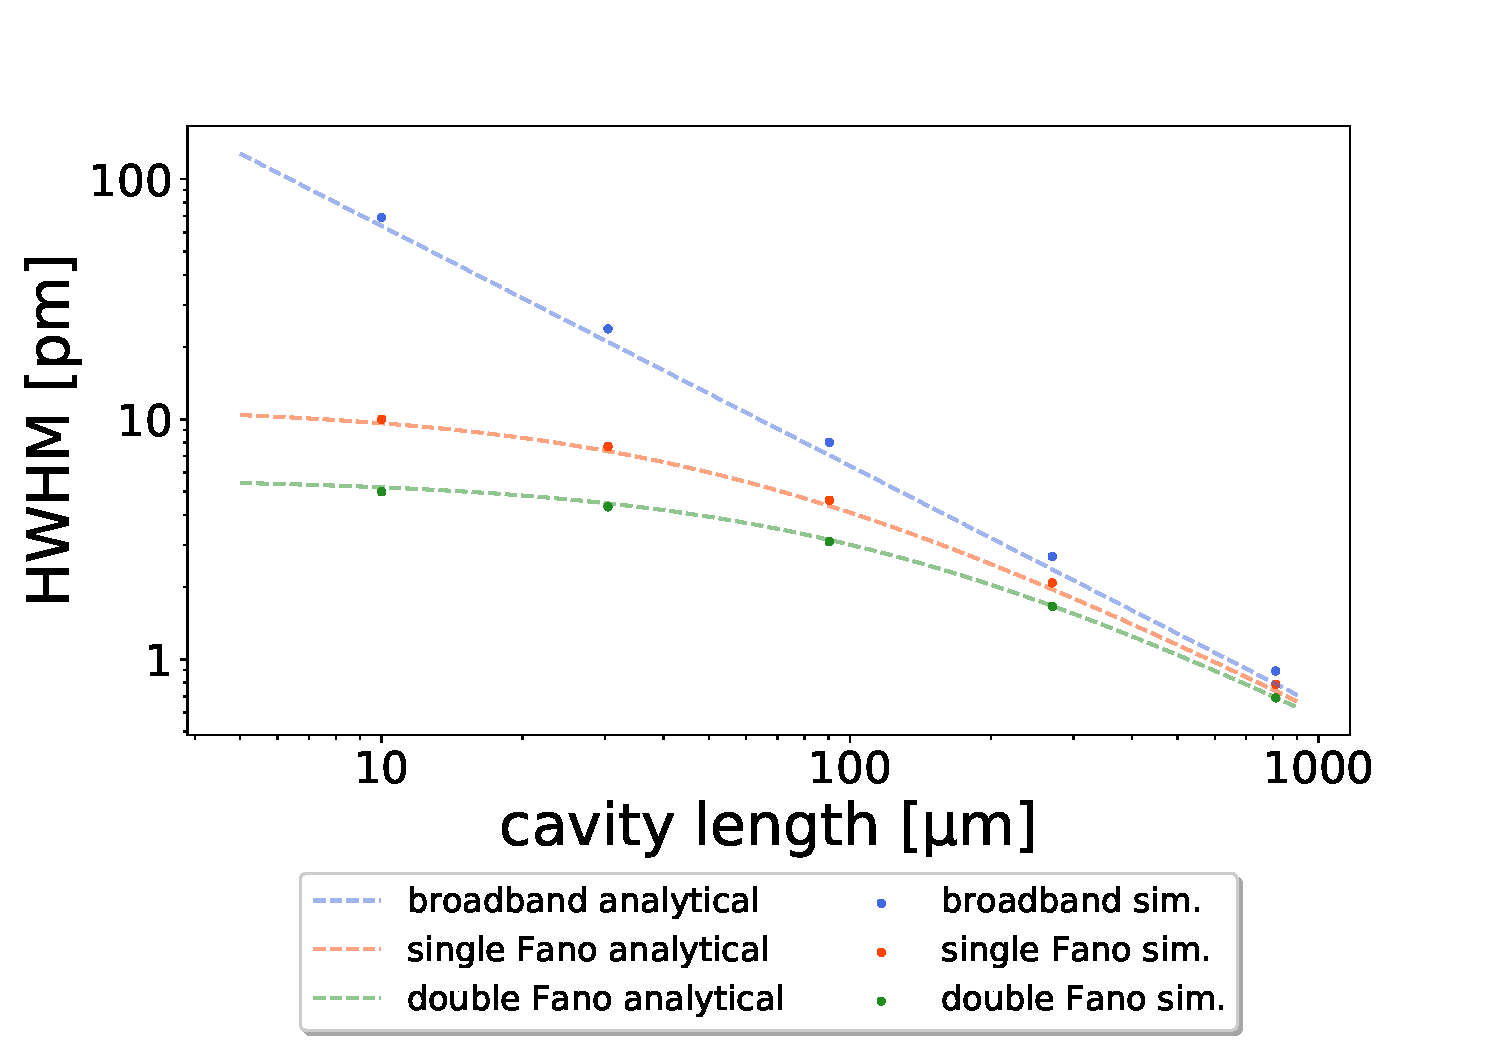
\includegraphics[width=\textwidth]{figures/HWHM_broadband_vs_single_vs_double_sim.pdf}
        \caption{}
        \label{fig:HWHM_double_vs_single_vs_broadband}
    \end{subfigure}
    \begin{subfigure}[c]{0.49\textwidth}
        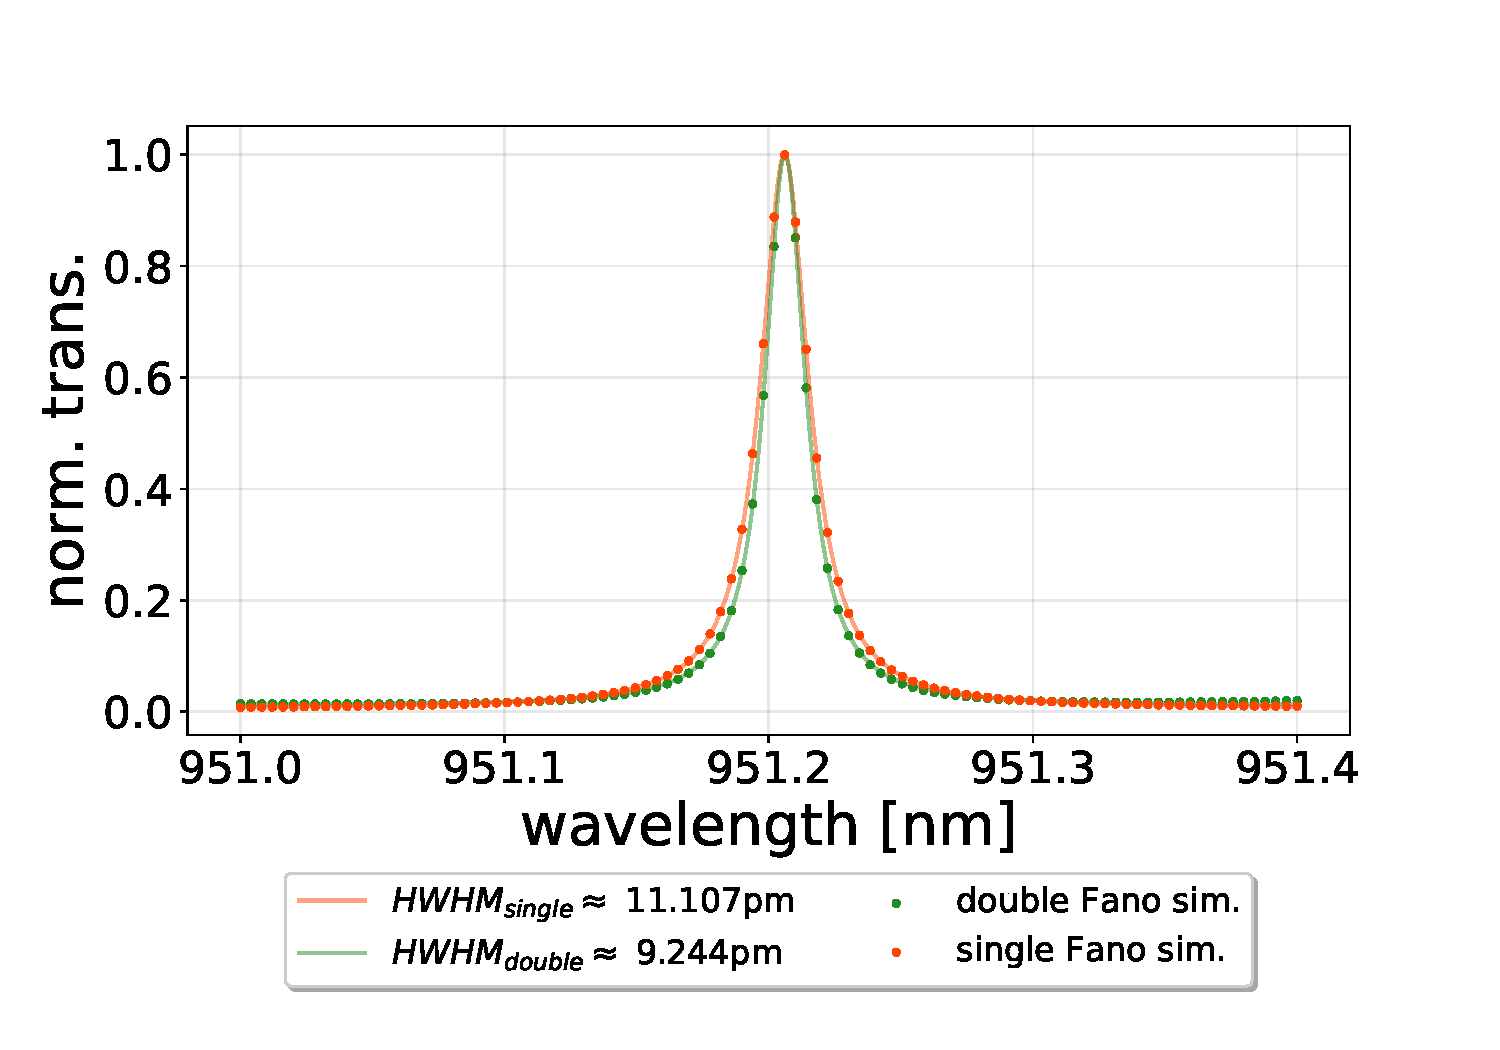
\includegraphics[width=\textwidth]{figures/sim_single_vs_double_270um.pdf}
        \caption{}
        \label{fig:700um_double_and_single_fano_peak}
    \end{subfigure}
    \begin{subfigure}[c]{0.49\textwidth}
        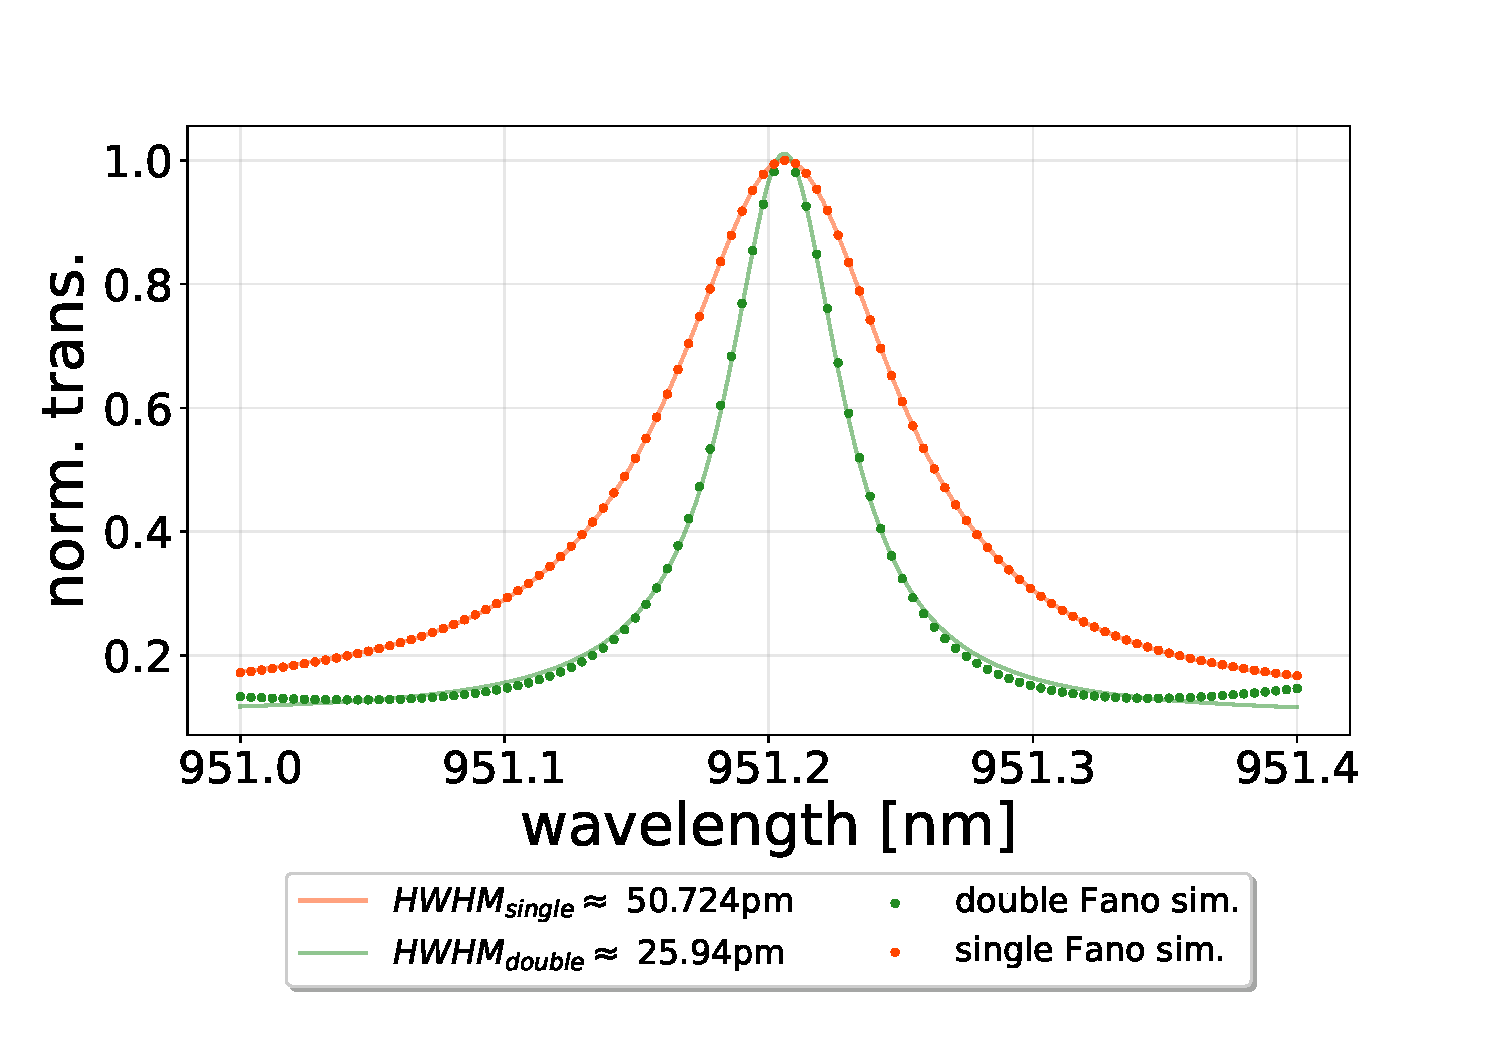
\includegraphics[width=\textwidth]{figures/sim_single_vs_double_10um.pdf}
        \caption{}
        \label{fig:10um_double_and_single_fano_peak}
    \end{subfigure}
    \caption{(a) shows the analytical resonance linewidths (eqs. (\ref{eq:analytical_linewidth}), (\ref{eq:analytical_linewidth_double}), and (\ref{eq:analytical_linewidth_broadband})) as a function of the cavity length for the broadband, single and double Fano cavities together with linewidths of corresponding profiles simulated using eqs. (\ref{eq:single_fano_trans}), (\ref{eq:double_fano_transmission}), and (\ref{eq:fabry_perot_trans}) for comparison. In (b) and (c) is seen transmission spectra of single and double Fano cavities of lengths $l \approx 270 \mu m$, and $l \approx 10 \mu m$, respectively. The spectra shown indicate each their respective linewidths, and are examples of the values plotted in (a). Note however, that the broadband cavity peak has been left out of (b) and (c).}
\end{figure}

Figure \ref{fig:HWHM_double_vs_single_vs_broadband} shows the analytical linewidth calculated and compared for the broadband, single Fano, and double Fano cavities, calculated using eqs. (\ref{eq:analytical_linewidth_broadband}), (\ref{eq:analytical_linewidth}), (\ref{eq:analytical_linewidth_double}). These are compared with linewidths found as fitting parameters from a least squares fit of the general Fano transmission formula given in eq. (\ref{eq:general_fano_model}) to transmission spectra calculated using eqs. (\ref{eq:fabry_perot_trans}), (\ref{eq:single_fano_trans}), and (\ref{eq:double_fano_transmission}). According to eq. (\ref{eq:analytical_linewidth_double}) the linewidth of the double Fano cavity transmission should converge to exactly half that of the single Fano cavity, meaning that
\begin{equation}
    \delta \lambda_{double} = \frac{\delta \lambda_{single}}{2}, \hspace{0.5cm} \text{for } l \rightarrow 0.
\end{equation}
This is supported well by the simulation depicted in figure \ref{fig:HWHM_double_vs_single_vs_broadband}.

Figures \ref{fig:700um_double_and_single_fano_peak} and \ref{fig:10um_double_and_single_fano_peak} contain examples of transmission spectra of single- and double Fano cavities and corresponding least squares fits to the general Fano model in order to determine their linewidths. 

\subsubsection{Additional cavity losses}\label{sec:additional_losses_theory}

Thus far we have only examined a lossless double Fano cavity where
\begin{equation}
    |r_g|^2 + |t_g|^2 = 1
\end{equation}
is fulfilled for both Fano mirrors used to contruct the cavity.

\begin{figure}[h!]
    \centering
    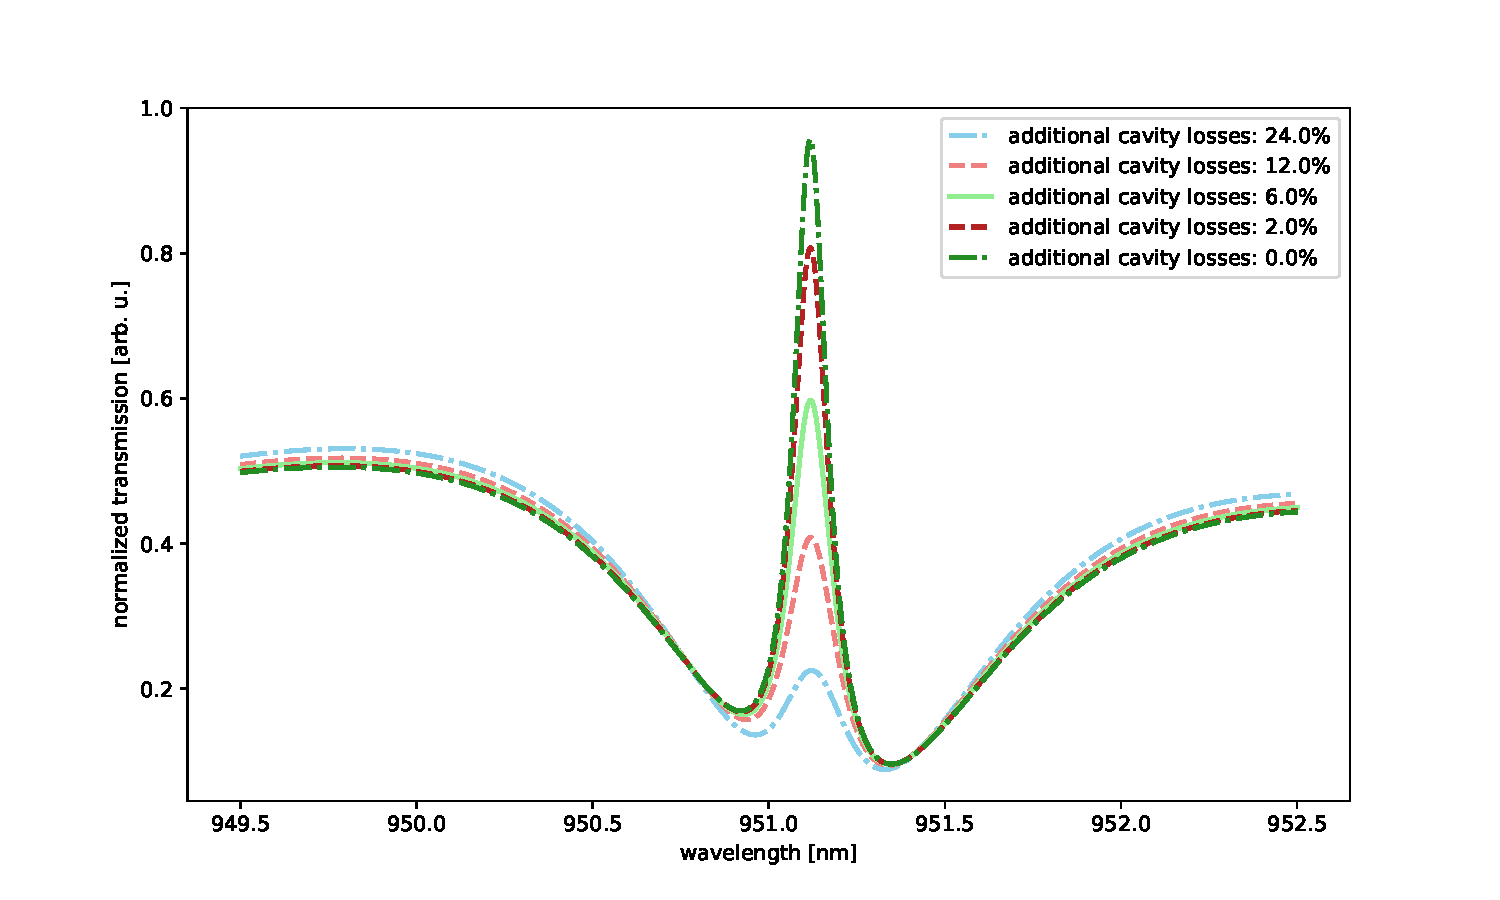
\includegraphics[width=0.6\textwidth]{figures/double_fano_loss_scan.pdf}
    \caption{Resonant transmission spectra for different values of the additional resonant loss term $L$, of a symmetric double Fano cavity of length $l \approx 30 \mu m$.}
    \label{fig:double_loss_scan}
\end{figure}

In this section we will investigate what happens when we introduce \emph{additional} cavity losses, not to be confused with the often used definition of cavity losses defined as $L=1-|r|^2$ where anything not being reflected back into the cavity is considered as "losses". Additional cavity losses, as described in this section, is given as
\begin{equation}
    L = 1 - |r_g|^2 - |t_g|^2,
\end{equation}
leading to the modified conervation condition
\begin{equation}
    |r_g|^2 + |t_g|^2 + L = 1.
\end{equation}

Figure \ref{fig:double_loss_scan} shows double Fano transmission spectra for a symmetric cavity with varying values for the additional cavity losses. It is readily seen that the maximum value reached in each spectrum is rapidly reduced with the introduction of these losses. 

Since the linewidth is defined as the HWHM of the transmission profile, this will naturally vary as a function of additional cavity losses. This is depicted in figure \ref{fig:HWHM_vs_losses} where the HWHM is shown for different values of $L$. Examples of transmission spectra taken for different values of $L$ are shown in figures \ref{fig:lossy_spectrum_0.2percent} and \ref{fig:lossy_spectrum_3.2percent}, along with their respective least squares fits to the general Fano model in eq. (\ref{eq:general_fano_model}) and linewidths found as fitting parameters hereof. 

\begin{figure}[h!]
    \centering
    \begin{subfigure}[c]{0.7\textwidth}
        \centering
        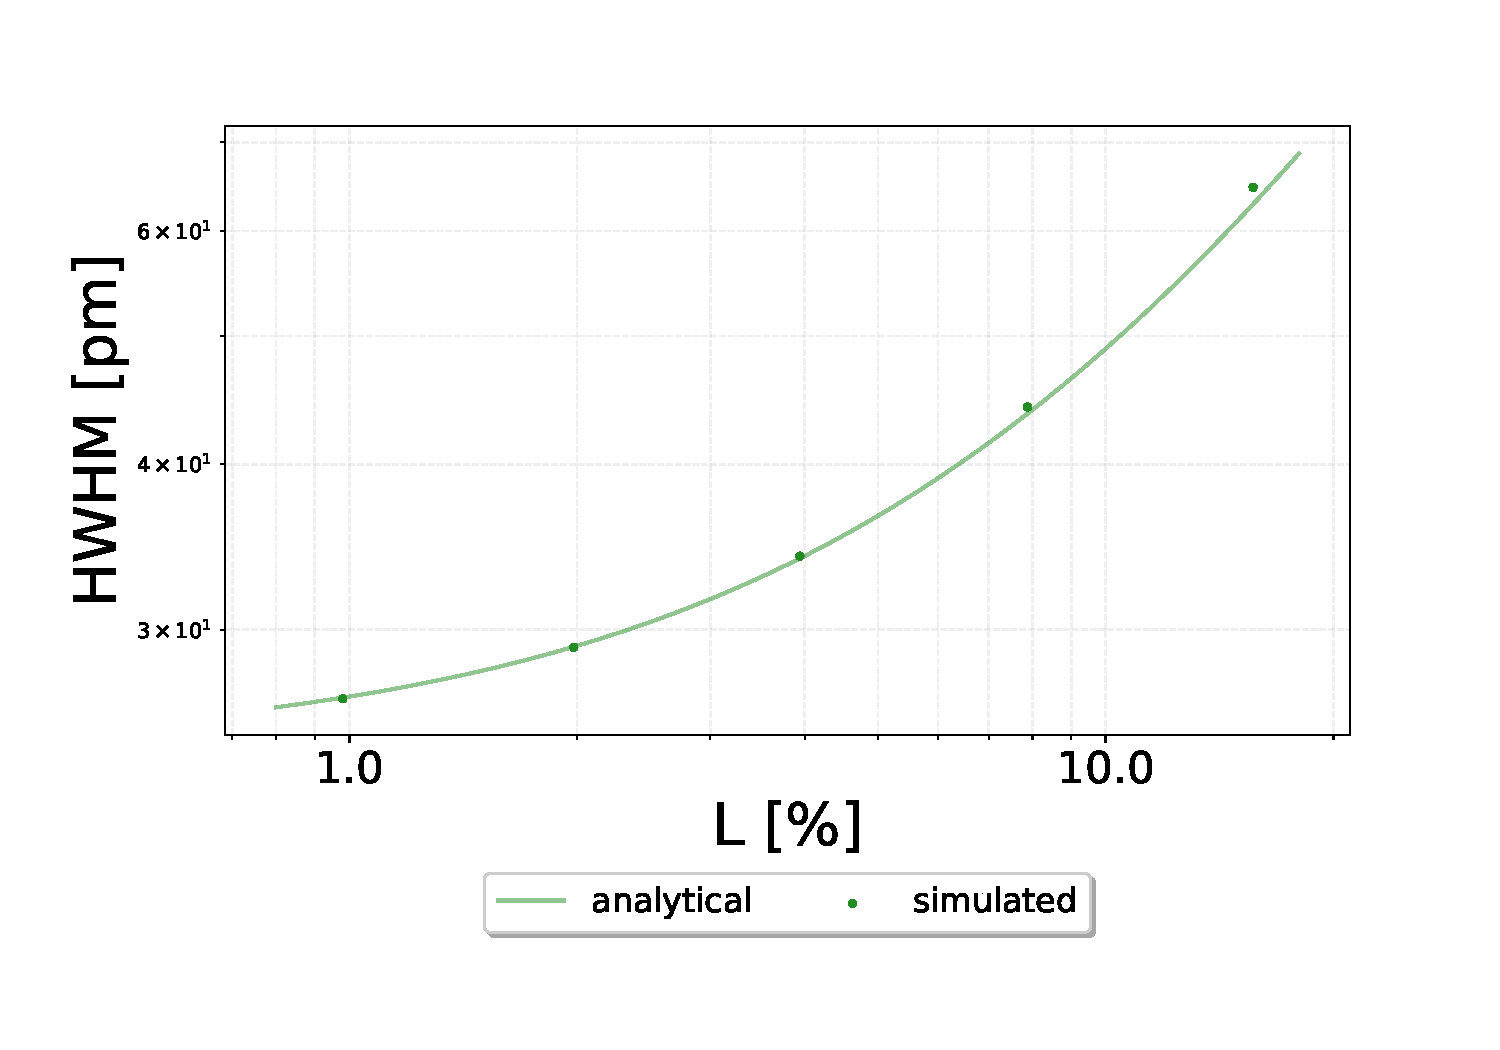
\includegraphics[width=\textwidth]{figures/linewidth_vs_losses.pdf}
        \caption{}
        \label{fig:HWHM_vs_losses}
    \end{subfigure}
    \begin{subfigure}[c]{0.49\textwidth}
        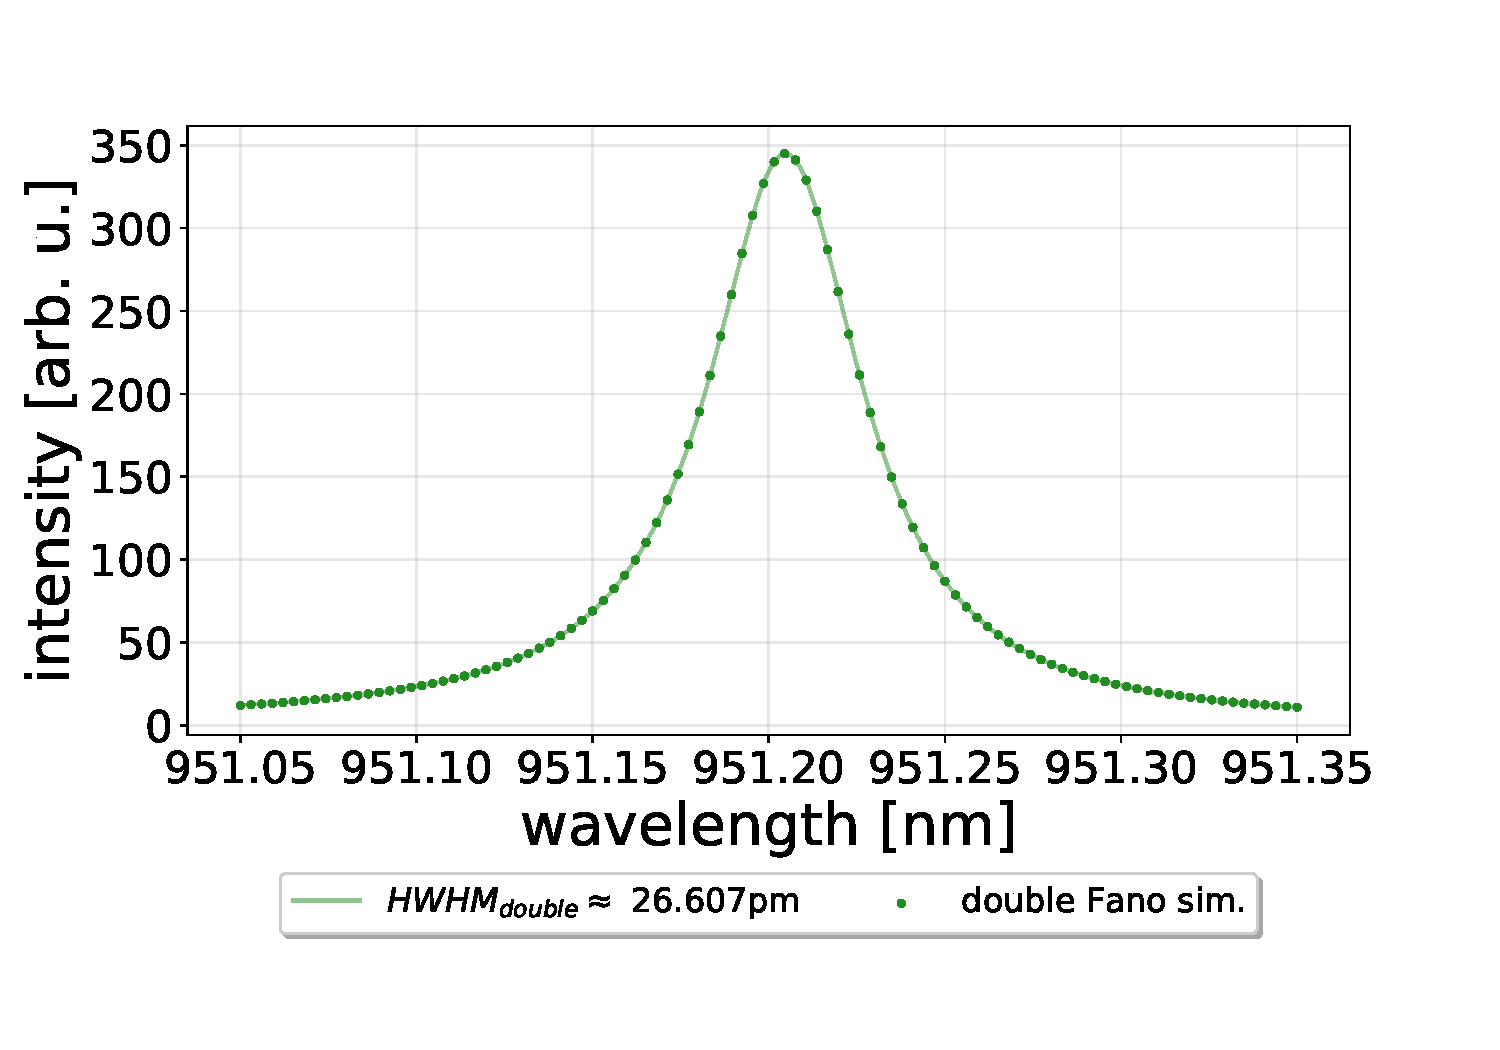
\includegraphics[width=\textwidth]{figures/double_1percent_loss_30um.pdf}
        \caption{}
        \label{fig:lossy_spectrum_0.2percent}
    \end{subfigure}
    \begin{subfigure}[c]{0.49\textwidth}
        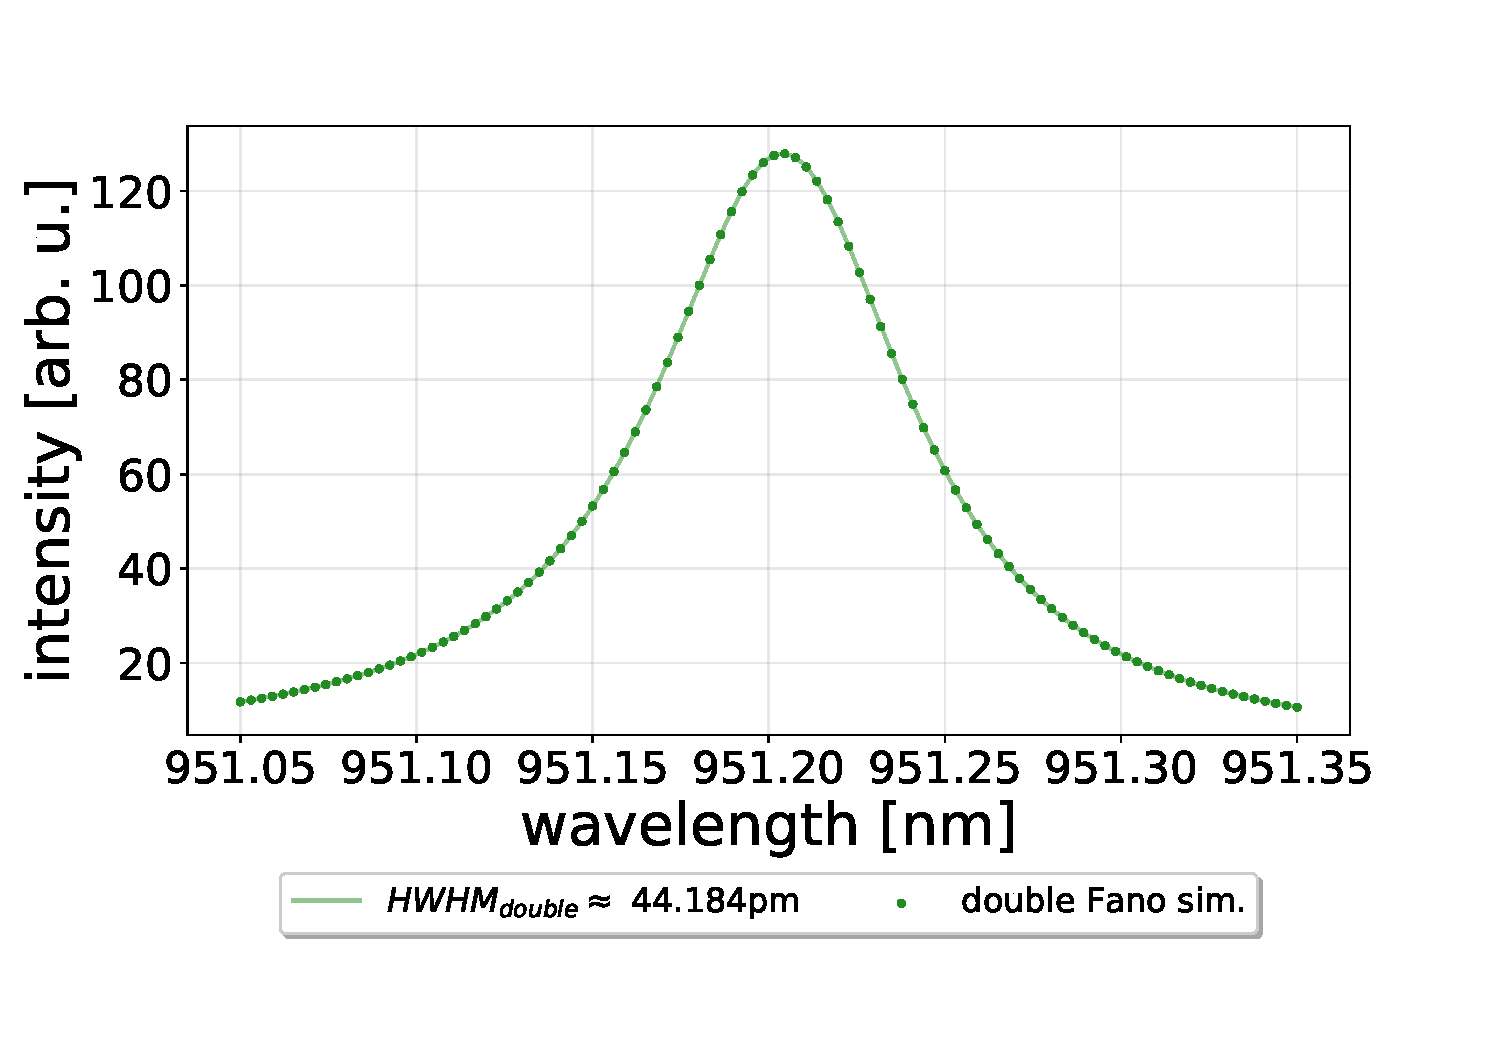
\includegraphics[width=\textwidth]{figures/double_8percent_loss_30um.pdf}
        \caption{}
        \label{fig:lossy_spectrum_3.2percent}
    \end{subfigure}
    \caption{(a) shows the linewidth (HWHM) of a symmetric double Fano cavity of length $l \approx 30 \mu m$  as a function of additional cavity losses $L = 2(1 - |r_g|^2 - |t_g|^2)$. Each point is found as a fitting parameter of a least squares fit of the double Fano intracavity spectrum for a certain value of $L$ to the general Fano model. The plotted line indicates the analytical value of the linewidth (eq. \ref{eq:analytical_linewidth}) as a function of $L$, for comparison. In (b) and (c) are seen examples of double Fano transmission spectra, with their respective linewidths, for cavities of $L=1\%$ and $L=8\%$, respectively.}
    \label{fig:HWHM_vs_losses_whole_figure}
\end{figure}

Figure \ref{fig:HWHM_vs_losses} shows the simulated linewidths of resonance transmission spectra as a function of the total additional cavity losses $L$, and is compared with the analytical formula for the double Fano linewidth in eq. (\ref{eq:analytical_linewidth_double}).

\subsubsection{Spectral detuning (lossless)} \label{sec:spectral_detuning}

Up until this point, it has been assumed that the Fano mirrors making up the double Fano cavity has been identical, namely the cavity has been \emph{symmetrical}. However, in practice this is very unlikely to be the case, as any Fano mirror constructed is bound to have some uncertainties attached to the physical parameters describing it (see eq. (\ref{eq:physical_grating_params})). For that reason we investigate the effect of an \emph{assymetric} cavity on the resulting transmission profile. Here we remember that each Fano mirror is describes by a set of parameters, $\lambda_0$, $\lambda_1$, $t_d$, $\gamma \lambda$ and $\beta$, which respectively describe the cavity resonance wavelength, guided-mode resonance wavelength, direct transmission, guided-mode resonance linewidth and additional losses of each grating. In order to model only a spectral detuning, we therefore simply change the parameters regarding the cavity and guided-mode resonance wavelengths, $\lambda_0$ and $\lambda_1$ by an amount corresponding to the detuning we wish to study. For this section the parameters will be given by the ones for the Fano mirror skecthed in figure \ref{fig:MIST_grating_sketch}, and thus given in eq. (\ref{eq:optical_grating_params}) for the unchanged Fano mirror, and
\begin{equation}
    \begin{split}
    \lambda_0^{\prime} = &\lambda_0 + \Delta,\:\: \lambda_1^{\prime} = \lambda_1 + \Delta,\:\: t_d^{\prime} = t_d,\\ &\gamma \lambda^{\prime} = \gamma \lambda\: \text{ and }\: \beta^{\prime} = \beta
    \end{split}
    \label{eq:detuned_grating_params}
\end{equation}
for the \emph{detuned} Fano mirror, where $\Delta$ is the detuning given by $\Delta = |\lambda_0 - \lambda_0^{\prime}|$. Figure \ref{fig:detuned_grating_spectra} shows the normalized reflectivity and transmission spectra of the unchanged Fano mirror (eq. (\ref{eq:optical_grating_params})) and the detunined Fano mirror (eq. (\ref{eq:detuned_grating_params})) for a detuning of $\Delta = 0.3$nm.

\begin{figure}[h!]
    \centering
    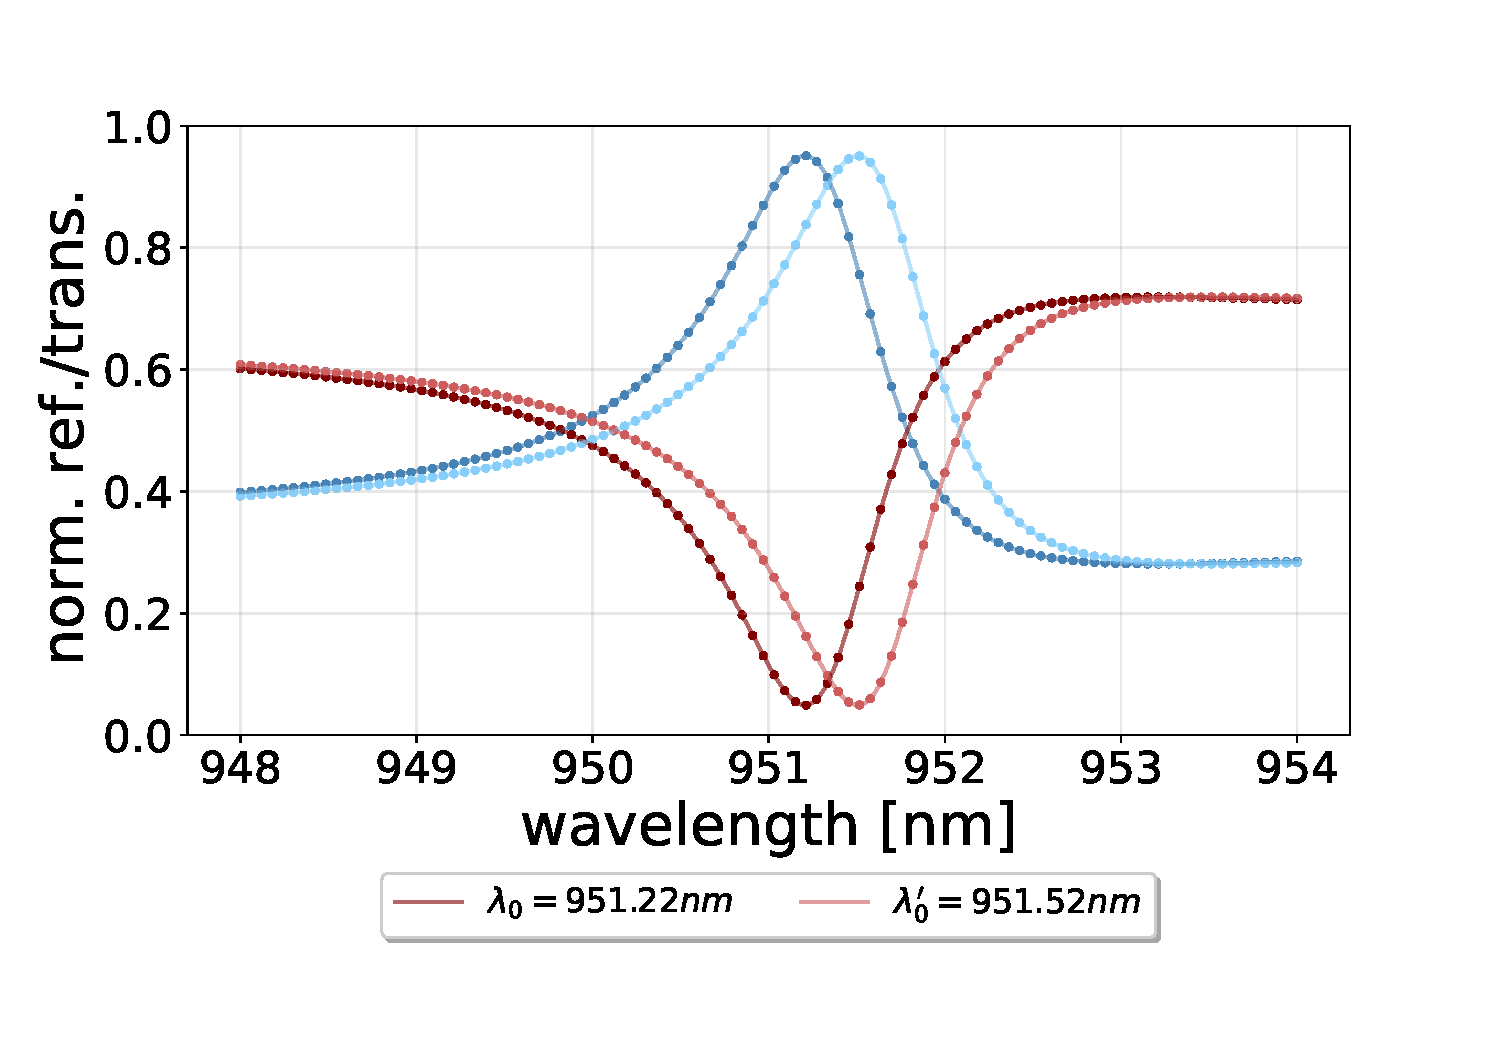
\includegraphics[width=0.7\textwidth]{figures/detuned_grating_spectra.pdf}
    \caption{The normalized reflectivity and transmission spectra of the Fano mirrors described in eqs. (\ref{eq:optical_grating_params}) and (\ref{eq:detuned_grating_params}) for detuning $\Delta = 0.3nm$.}
    \label{fig:detuned_grating_spectra}
\end{figure}

As has been observed in previous sections, the Fano resonance transmission peak is present at the point where the grating reflectivity $r_g(\lambda)$ is maximized and transmission $t_g(\lambda)$ minimized. However, when $\lambda_0 \neq \lambda_0^{\prime}$ and $\lambda_1 \neq \lambda_1^{\prime}$, this is no longer a trivial conclusion to draw. The question of whether the cavity resonance should be tuned to match the guided-mode resonance wavelength of one grating or the other, or maybe somewhere in between does not have an obvious answer. This will be further expanded upon later in section \ref{sec:spacial_detuning}, but in order to move forward with the investigation of the spectral detuning we, for now, accept that the optimal cavity length, is the one corresponding to a cavity resonance $\lambda_t$ given, exactly between the two guided-mode resonance wavelengths, as 
\begin{equation}
    \lambda_t = \frac{\lambda_{0} + \lambda_{0}^{\prime}}{2}.
    \label{eq:transmission_wavelength}
\end{equation}
Where \emph{t} is for \emph{transmission} as this is, later on, to be used experimentally as the \emph{transmission wavelength}. 

\begin{figure}[h!]
    \centering
    \begin{subfigure}[b]{0.49\textwidth}
        \centering
        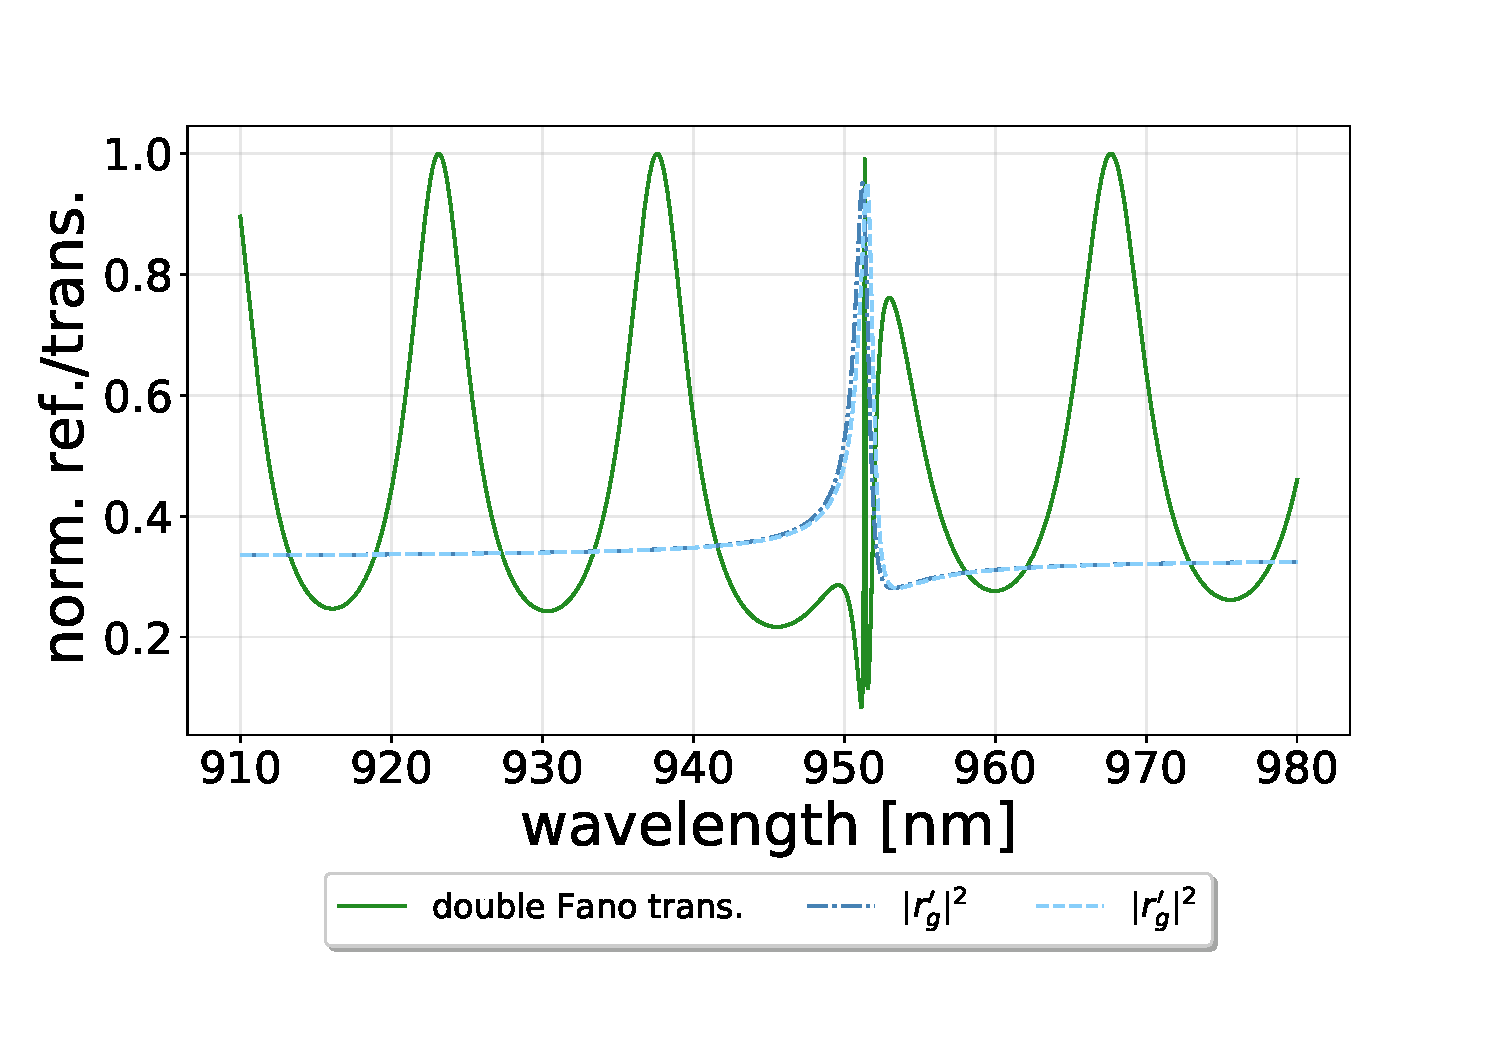
\includegraphics[width=\textwidth]{figures/detuned_full_range_double_trans.pdf}
        \caption{}
        \label{fig:full_range_detuned_trans}
    \end{subfigure}
    \begin{subfigure}[b]{0.49\textwidth}
        \centering
        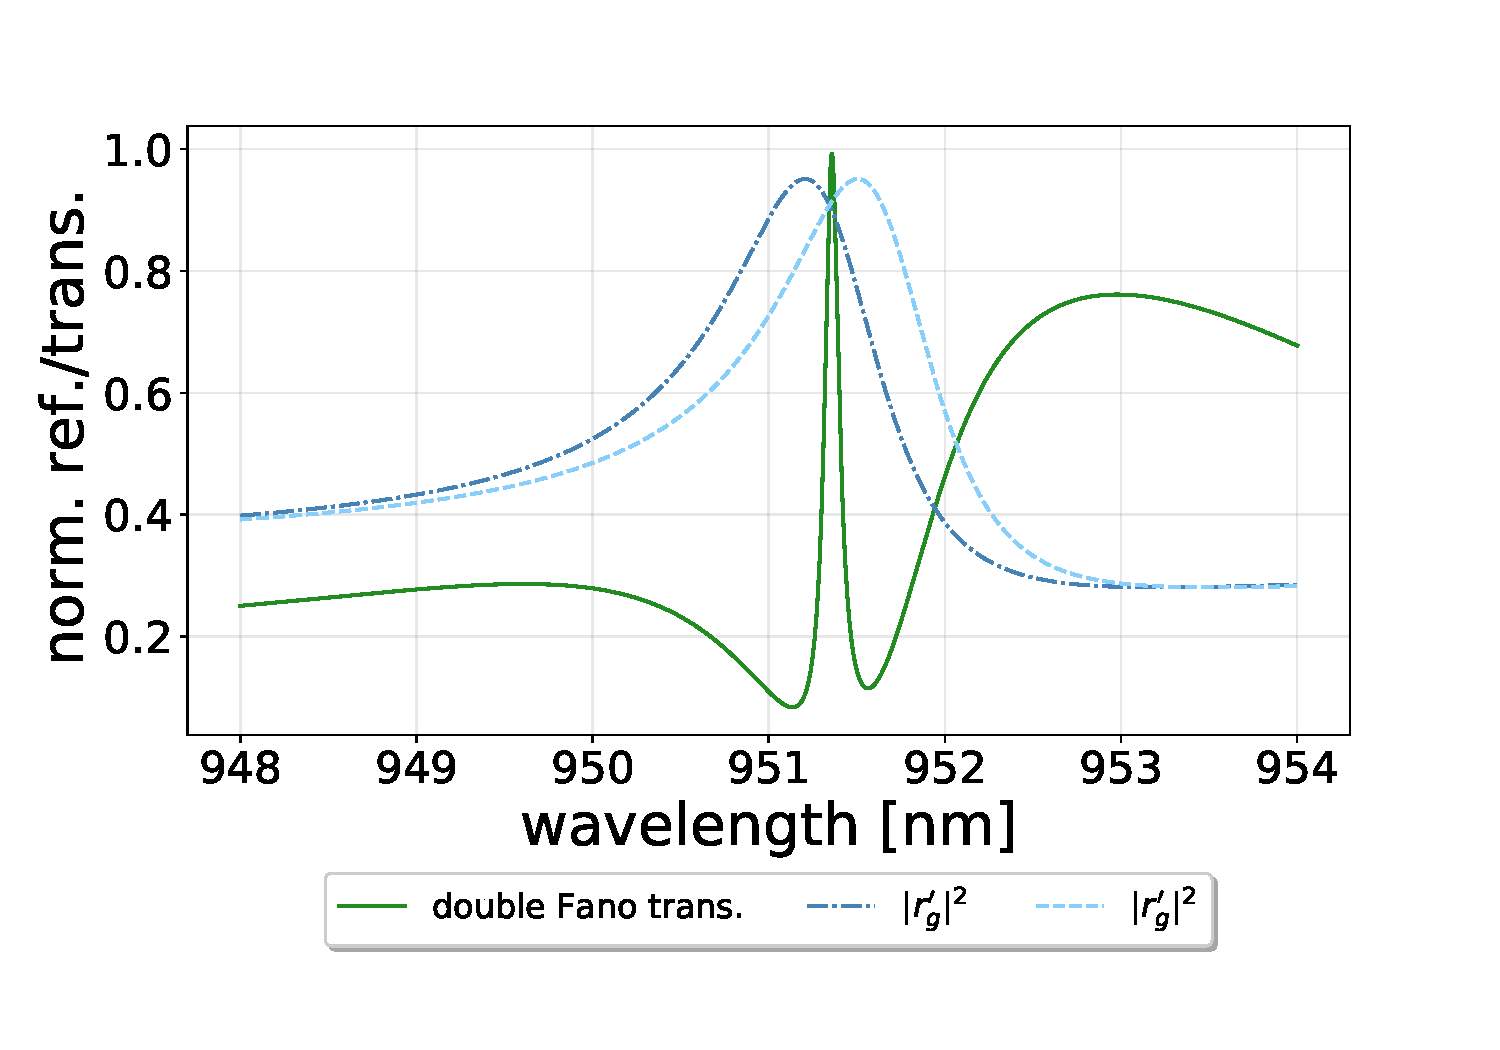
\includegraphics[width=\textwidth]{figures/detuned_short_range_double_trans.pdf}
        \caption{}
        \label{fig:short_range_detuned_trans}
    \end{subfigure}
    \caption{The double Fano transmission spectra of a cavity of length $l \approx 30 \mu m$ and detuned by $\Delta = 0.3$nm, as seen in figure \ref{fig:detuned_grating_spectra}, together with the reflectivity spectra of the Fano mirrors used for the simulation.}
    \label{fig:detuned_double_fano_transmission}
\end{figure}

Figure \ref{fig:detuned_double_fano_transmission} shows the transmission spectrum of a detuned double Fano cavity with parameters corresponding to the transmission and reflectivity spectra in figure \ref{fig:detuned_grating_spectra}, meaning that $\Delta = 0.3$nm. The transmission wavelength $\lambda_t$ is chosen such that eq. (\ref{eq:transmission_wavelength}) is fulfilled, and correspondingly it is seen that the transmission peak is placed exactly between the maximum (minimum) reflectivites (transmissions) of the two grating, i.e. between the two guided-mode resonance wavelengths. Furthermore, it can be concluded that the detuning is chosen such that the overlap between the guided-mode resonances is still substantiel enough for them to couple and hence for the overall Fano resonance to be excited. 

While knowing that a detuning of $0.3$nm is acceptable in terms of exciting the Fano resonance in the lossless case is a nice result, it does not provide much in terms of estimating the acceptable detuning for any experimental purposes. In figure \ref{fig:detuning_scan} the double Fano transmission is shown for increasing detuning $\Delta$ and transmission wavelength $\lambda_t = (\lambda_{0} + \lambda_{0}^{\prime}(\Delta))/2$. 

\begin{figure}[h!]
    \centering
    \begin{subfigure}[b]{0.49\textwidth}
        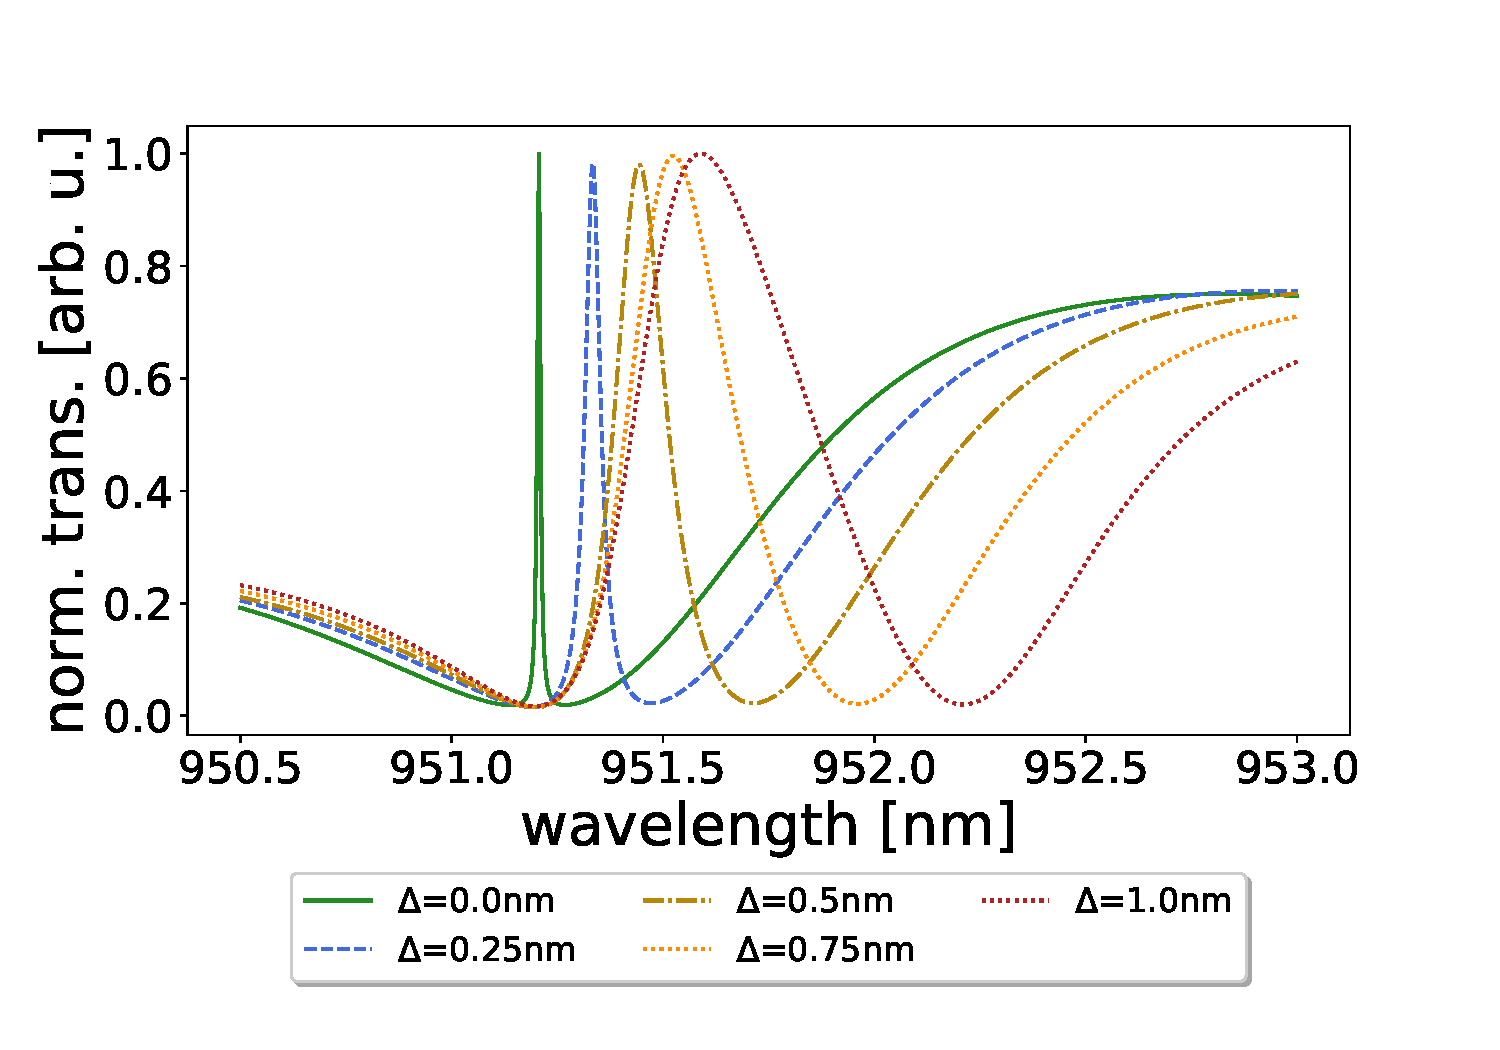
\includegraphics[width=\textwidth]{figures/detuning_scan_double_fano_30um.pdf}
        \caption{}
        \label{fig:detuning_scan}
    \end{subfigure}
    \begin{subfigure}[b]{0.49\textwidth}
        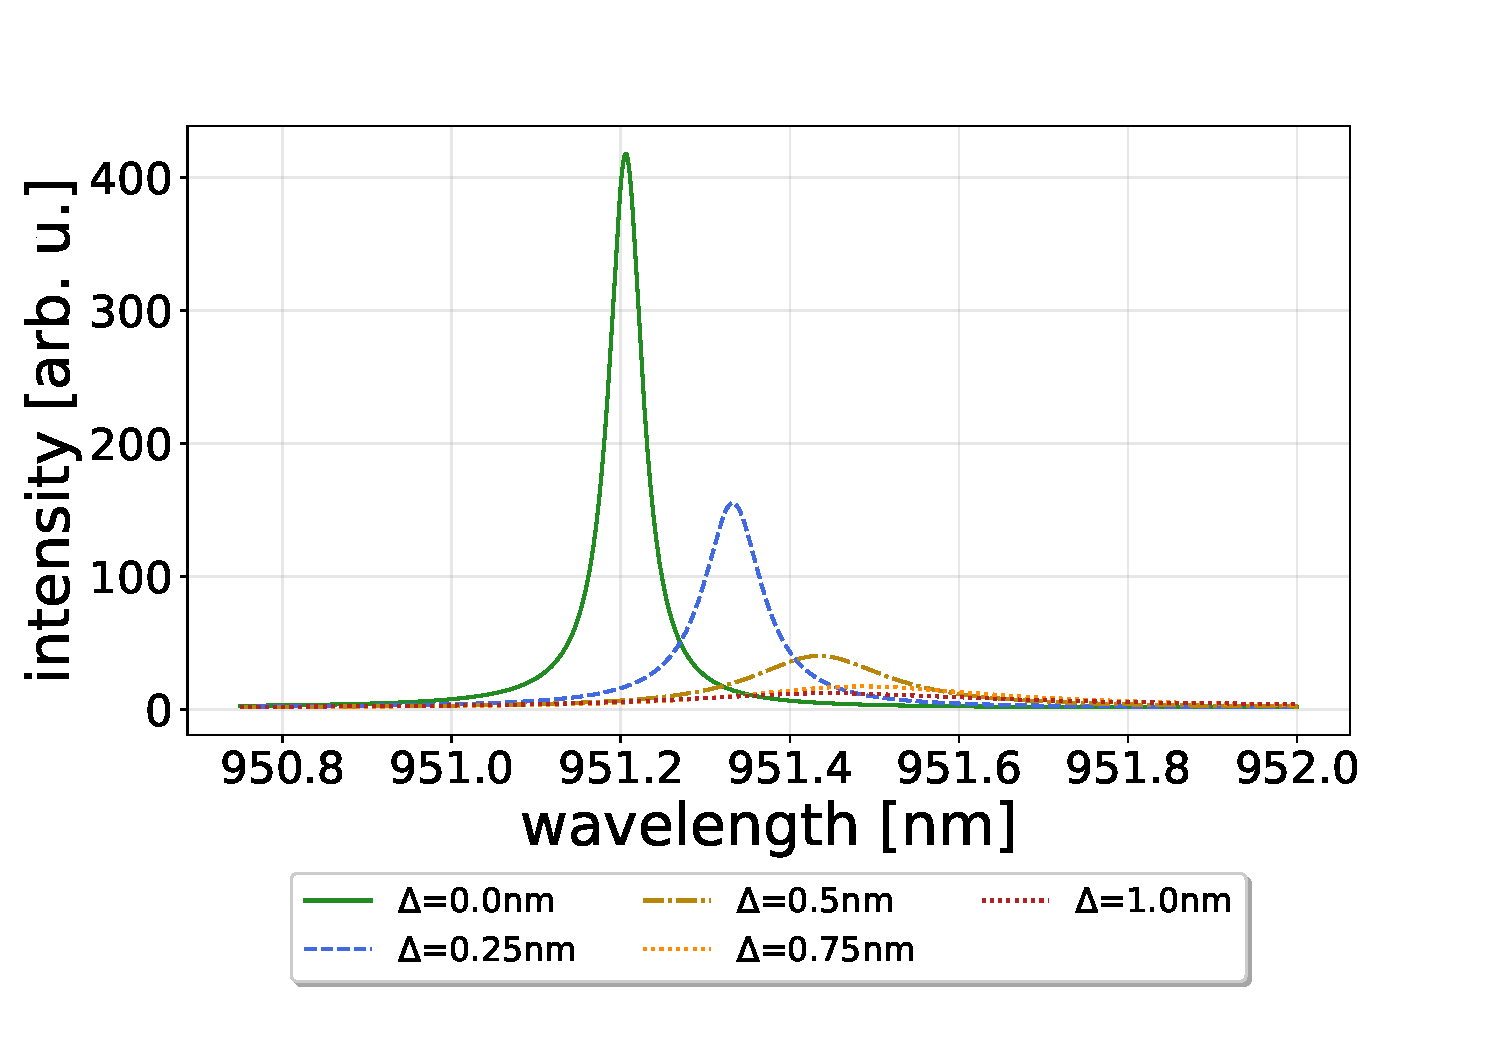
\includegraphics[width=\textwidth]{figures/detuning_scan_double_fano_30um_intracavity.pdf}
        \caption{}
        \label{fig:detuning_scan_intracavity}
    \end{subfigure}
    \caption{In (a) is seen lossless double Fano transmission spectra for increasing value of the detuning $\Delta = |\lambda_{0} - \lambda_{0}^{\prime}|$. It is readily seen that the transmission wavelength $\lambda_t = (\lambda_{0} + \lambda_{0}^{\prime})/2$ becomes higher, and that the linewidth likewise becomes larger with increasing detuning. (b) shows the intracavity spectra corresponding to the transmission spectra in (a) normalized by each their maximum value, shown in (c), in order to preserve readability.}
    \label{fig:detuning_scans}
\end{figure}

It is readily seen that with increasing positive detuning, relative to the resonant wavelength of the unchanged Fano mirror, the peak shifts to higher wavelengths, which in itself is easily seen from eq. (\ref{eq:transmission_wavelength}). The linewidth is also seen to increase with the detuning, and the peak will eventually collapse when the overlap between the guided-mode resonance profiles of the two Fano mirrors becomes too small to sustain the Fano resonance. This collapse was seen for examples of higher losses, and will be evident in later sections. Figure \ref{fig:detuning_scan_intracavity_normalized} shows the intracavity spectra corresponding to the transmission spectra in figure \ref{fig:detuning_scan} normalized by their respective maximum values plotted in figure \ref{fig:detuning_scan_intracavity_max_values} in order to preserve readability. The intracavity spectra provides valuable insight into the mode density inside the cavity for the different values of $\Delta$, and considering the significant difference of $\propto 10^4$ in the maximum value for the intensity, a mode density decrease is, though qualitative, clearly shown by figure \ref{fig:detuning_scan_intracavity_max_values}.  

It is clearly demonstrated by figures \ref{fig:detuning_scan}, \ref{fig:detuning_scan_intracavity_normalized} and \ref{fig:detuning_scan_intracavity_max_values} that the spectral overlap is a very crucial parameter of the double Fano cavity, and is paramount in describing the cavity's ability to produce narrow Fano resonant structures. 

\subsubsection{Spacial detuning (lossless)} \label{sec:spacial_detuning}

As mentioned above in section \ref{sec:spectral_detuning}, any spectral detuning gives rise to the potential of a spacial detuning as $2l = m\lambda$ must be fulfilled for any sustained plane-wave mode inside a normal incident optical cavity. We denote the length corresponding to the resonance wavelength of the unchanged Fano mirror as simply $l$, while the one for the detuned Fano mirror will be denoted as $l^{\prime}$. Previously we assumed that the optimal length of a detuned double Fano cavity is the one where the so-called transmission wavelength is given as 
\begin{equation}
    \lambda_t = \frac{\lambda_{0} + \lambda_{0}^{\prime}}{2}.
\end{equation}
And while this does turn out to be a good emprically justified assumption in the experimental part of this project, we will model and investigate the resonant length-dependence of the linewidth of the Fano resonance profile. 

\begin{figure}[h!]
    \centering
    \begin{subfigure}[b]{0.49\textwidth}
        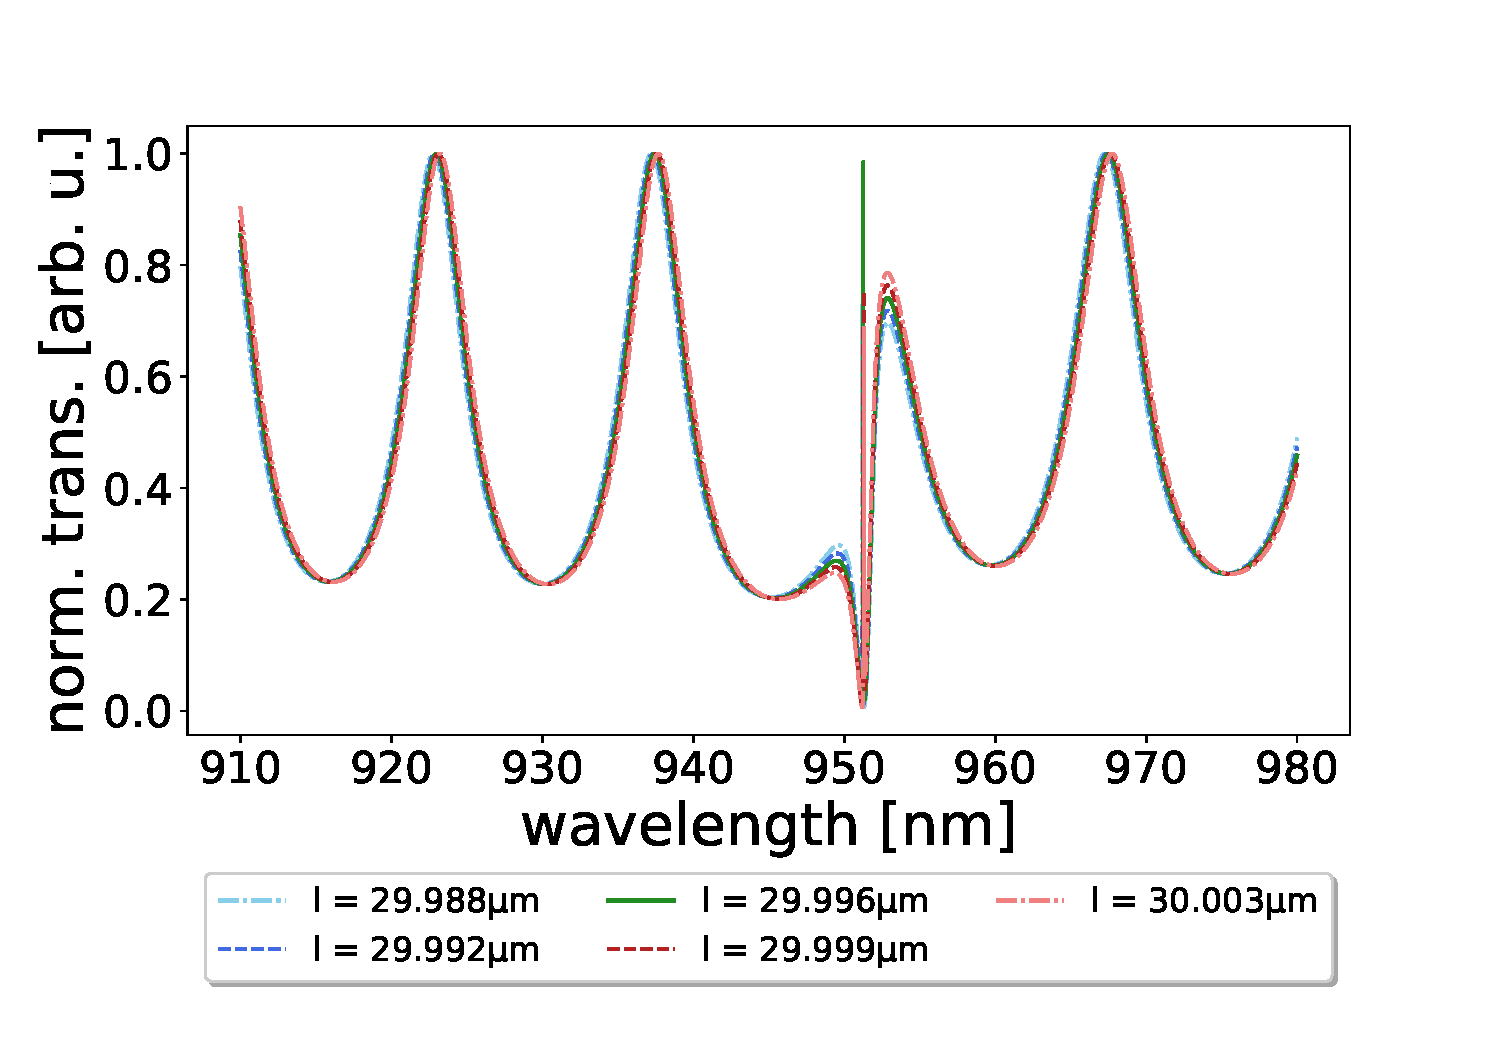
\includegraphics[width=\textwidth]{figures/small_detuning_length_scan_long.pdf}
        \caption{}
        \label{fig:detuned_small_length_scan_long}
    \end{subfigure}
    \begin{subfigure}[b]{0.49\textwidth}
        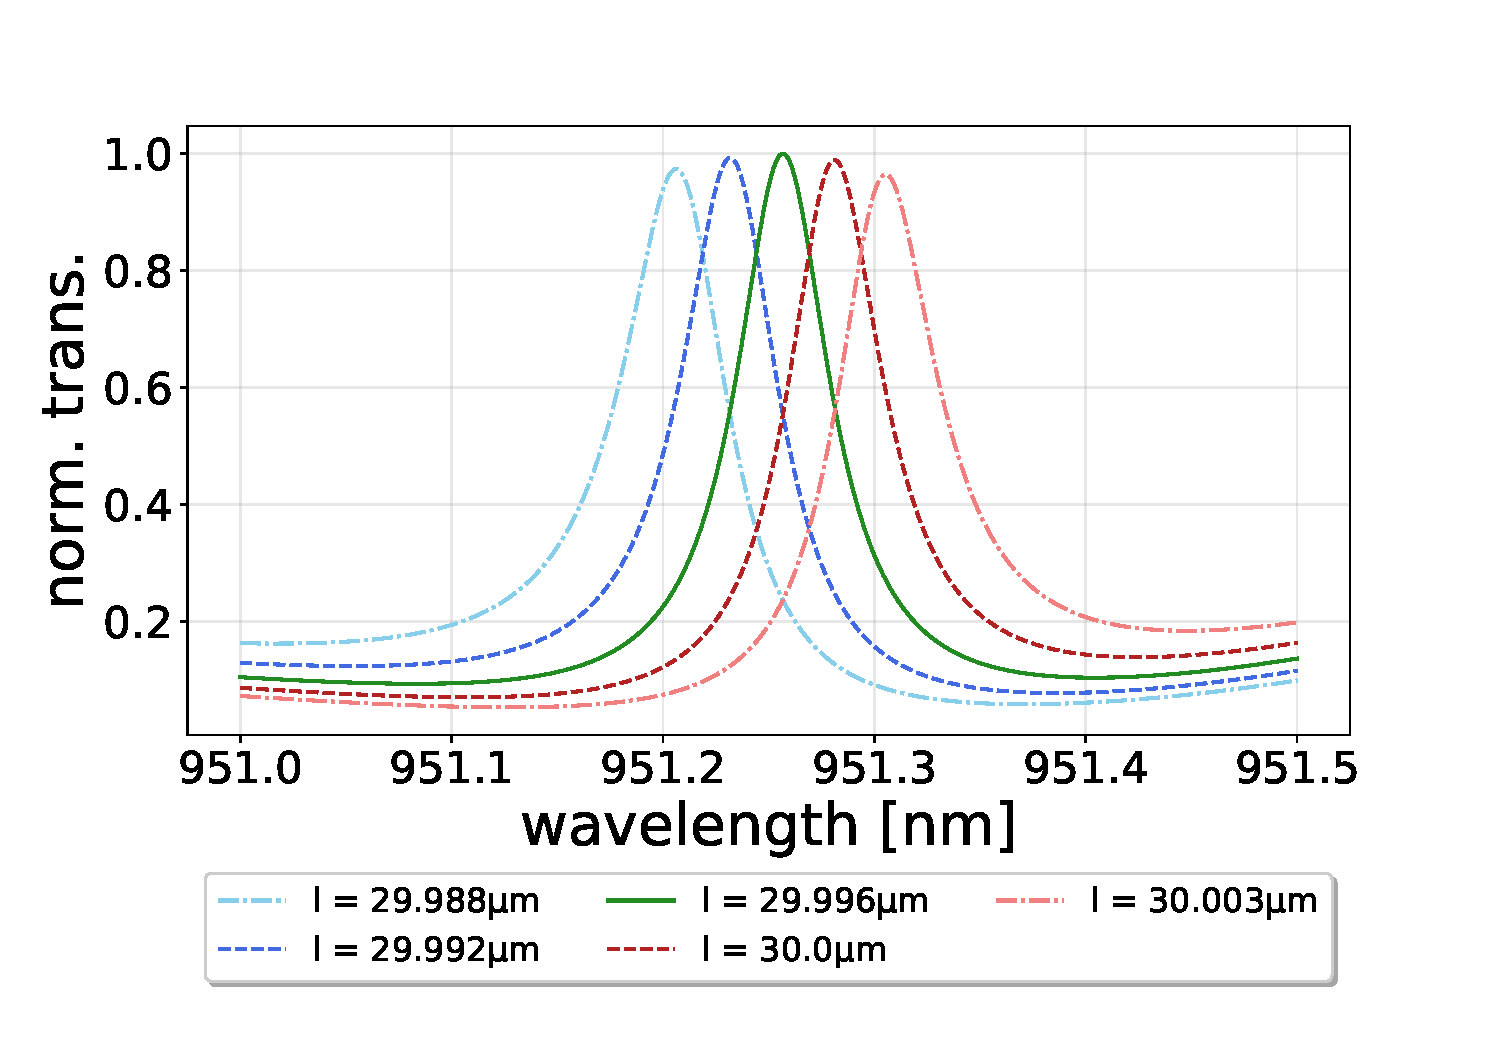
\includegraphics[width=\textwidth]{figures/small_detuning_length_scan_short.pdf}
        \caption{}
        \label{fig:detuned_small_length_scan_short}
    \end{subfigure}
    \caption{(a) shows lossless long-range transmission spectra of double Fano cavities of lengths $l \rightarrow l^{\prime} \approx 30 \mu m$ with $\Delta = 0.1nm$. (b) shows the same spectra as seen in (a), zoomed in on the range around the transmission wavelength $\lambda_t$.}
    \label{fig:small_detuning_length_scans}
\end{figure}

Figure \ref{fig:small_detuning_length_scans} shows double Fano resonance transmission profiles plottet for varying cavity length $l \rightarrow l^{\prime}$ with detuning $\Delta = 0.1nm$. The long range wavelength scan in figure \ref{fig:detuned_small_length_scan_long} shows a well-defined off-resonance behavior, as the detuning is barely visible on this scale, while the peak height on resonance is already visibly affected. The immediate off-resonance spectra also shows visible changes as the peak "background" level depend heavily on the location of the overall resonance.  

Figure \ref{fig:detuned_small_length_scan_short} shows the same spectra, but enhanced around the resonance wavelength. This shows that the substantiel guided-mode overlap, and thus small detuning, is enough to detect significant changes in the reosnance spectra. The shifting of the peak position is evident, but the most prominent change is seen in the peak height, which is reduced from $1$ when $\lambda_t = (lambda_0 + \lambda_0^{\prime})/2$ to around $0.8$ when $\lambda_t = lambda_0$ or $\lambda_t = \lambda_0^{\prime}$.

\begin{figure}[h!]
    \centering
    \begin{subfigure}[b]{0.49\textwidth}
        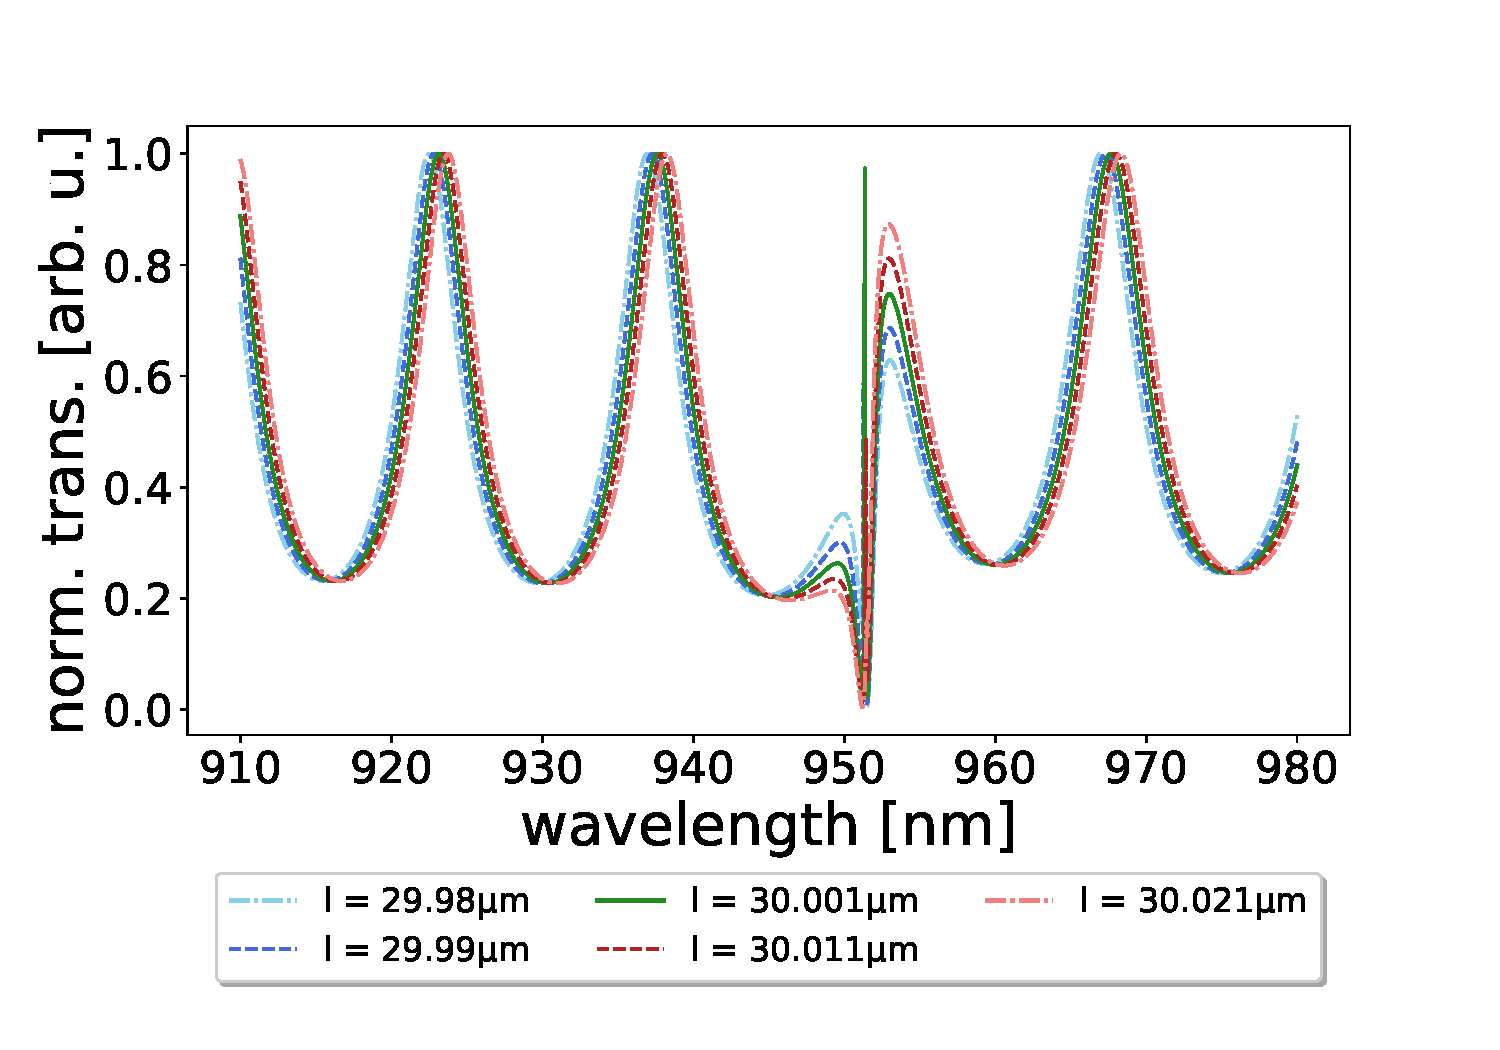
\includegraphics[width=\textwidth]{figures/medium_detuning_length_scan_long.pdf}
        \caption{}
        \label{fig:detuned_length_scan_long}
    \end{subfigure}
    \begin{subfigure}[b]{0.49\textwidth}
        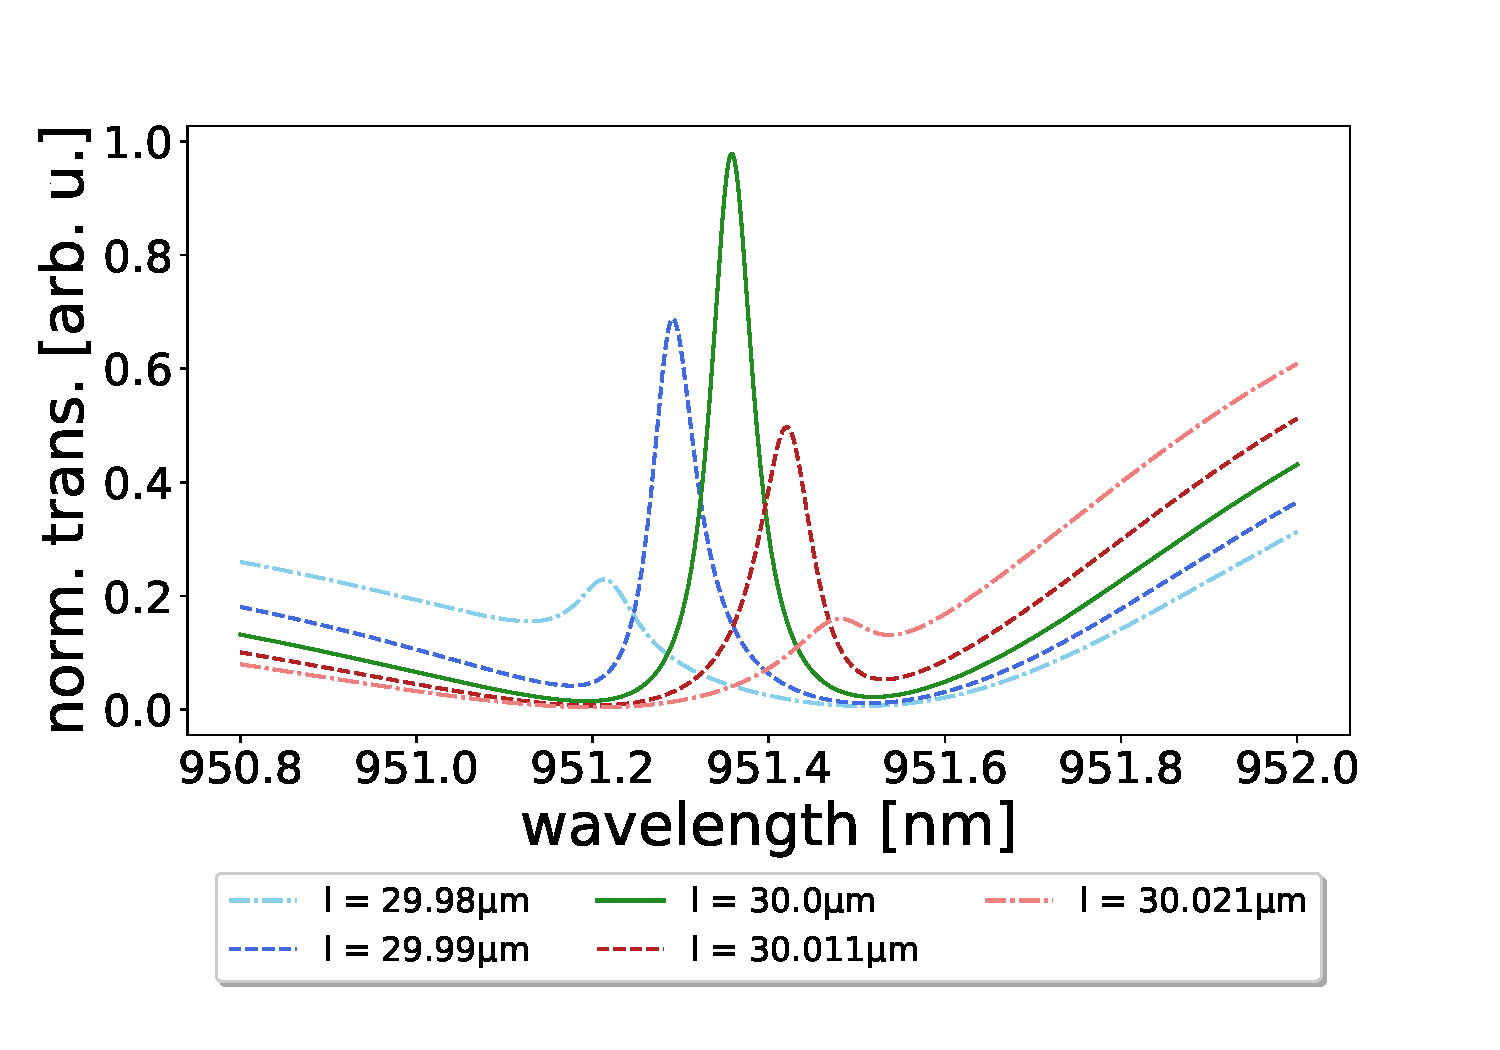
\includegraphics[width=\textwidth]{figures/medium_detuning_length_scan_short.pdf}
        \caption{}
        \label{fig:detuned_length_scan_short}
    \end{subfigure}
    \caption{(a) shows lossless long-range transmission spectra of double Fano cavities of lengths $l \rightarrow l^{\prime} \approx 30 \mu m$ with $\Delta = 0.3nm$. (b) shows the same spectra as seen in (a), zoomed in on the range around the transmission wavelength $\lambda_t$.}
    \label{fig:mid_detuning_length_scans}
\end{figure}

Figure \ref{fig:mid_detuning_length_scans} shows similar transmission profiles as in figure \ref{fig:small_detuning_length_scans}, only with an increased detuning of $\Delta = 0.3$nm. Looking at the long range scan in figure {\ref{fig:detuned_length_scan_long}} and comparing with the one in figure \ref{fig:detuned_small_length_scan_long}, it is seen that the displacement of the off-resonance Fabry-Perot like fringes have increased with the slightly higher detuning. This is not surprising as the Fabry-Perot cavity modes, like any other interference pattern inside a cavity must fulfill the brightness identity $2l = m \lambda$. Furthermore, the immediate off-resonance regime shows an increase in the intensity displacement when compared with the less detuned example. 

Figure \ref{fig:detuned_length_scan_short}, which shows the spectra enhanced around the resonance position, provides a more detailed image of what happens to the transmission profiles as a function of the cavity length. Here it is seen that the peaks at the edges of the length interval have varied even more in shape, height and linewidth than in figure \ref{fig:detuned_length_scan_short}. In short, the increased detuning has also increased the fractional length-dependence of the double Fano cavity transmission profile. Here it must however be noted here that the range in which the cavity length is scanned is increased with the detuning. So the length-dependence is fractional in the sense that the step size is here defined by the size of the interval.

\begin{figure}[h!]
    \centering
    \begin{subfigure}[b]{0.49\textwidth}
        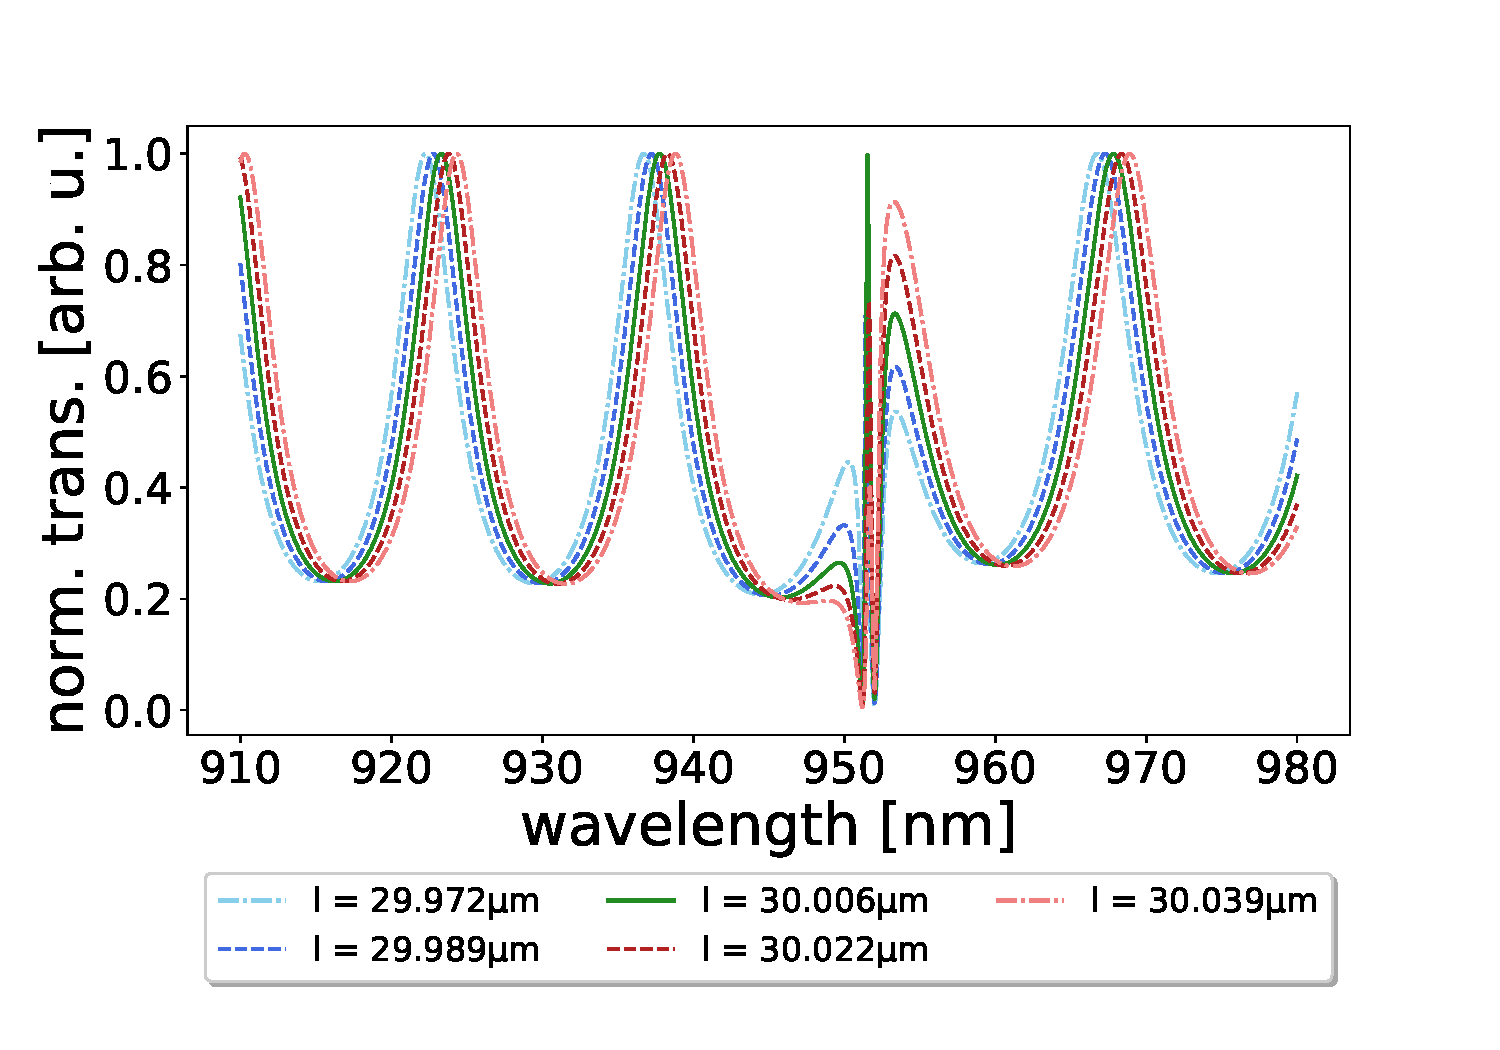
\includegraphics[width=\textwidth]{figures/large_detuning_length_scan_long.pdf}
        \caption{}
        \label{fig:detuned_large_length_scan_long}
    \end{subfigure}
    \begin{subfigure}[b]{0.49\textwidth}
        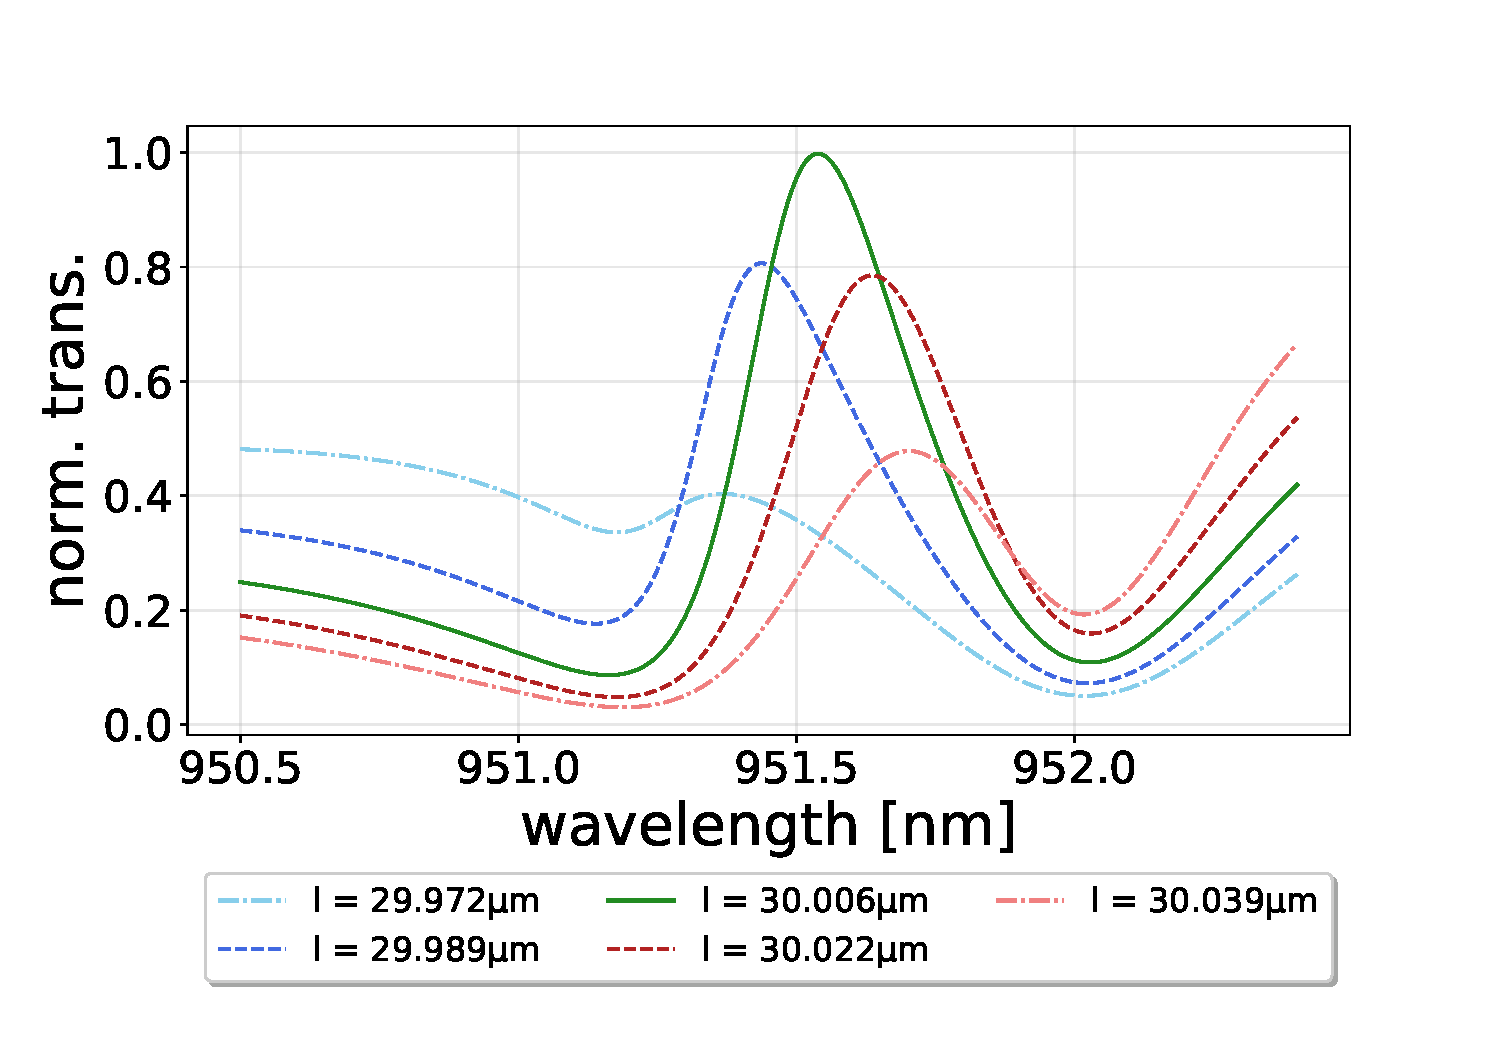
\includegraphics[width=\textwidth]{figures/large_detuning_length_scan_short.pdf}
        \caption{}
        \label{fig:detuned_large_length_scan_short}
    \end{subfigure}
    \caption{(a) shows lossless long-range transmission spectra of double Fano cavities of lengths $l \rightarrow l^{\prime} \approx 30 \mu m$ with $\Delta = 0.8nm$. (b) shows the same spectra as seen in (a), zoomed in on the range around the transmission wavelength $\lambda_t$.}
    \label{fig:large_detuning_length_scans}
\end{figure}

Figure \ref{fig:large_detuning_length_scans} shows the effect of a relatively large detuning of $\Delta = 0.8$nm. This is simply included for a visual representation of a detuning which is considered "too large" for any practical use. The long range scan in figure \ref{fig:detuned_large_length_scan_long} shows that the Fabry-Perot like fringes are now even more displaced, and figure \ref{fig:detuned_large_length_scan_short} showing the spectra enhanced around the resonance wavelength shows roughly the same trend as in figure \ref{fig:detuned_length_scan_short}, only that this example is greatly broadened in comparison. It is though noted, that while broadened, the Fano resonance mode is sustained even for the relatively large detuning.

In order to get a clear qualitative picture of the double Fano cavity transmission profile as a function of both cavity length and wavelength, we visualize the varying of both in a heat map and let the color indicate the transmission intensity. This is shown in figure \ref{fig:cmap_single} which depicts a lossless cavity of length $l\approx 30 \mu m$ and detuning $\Delta = 0.3$nm. Here the movement of the resonance peak as a function of the cavity length is clearly seen as a slope of the "line" representing the high intensity region due to the Fano resonance. 

\begin{figure}[h!]
    \centering
    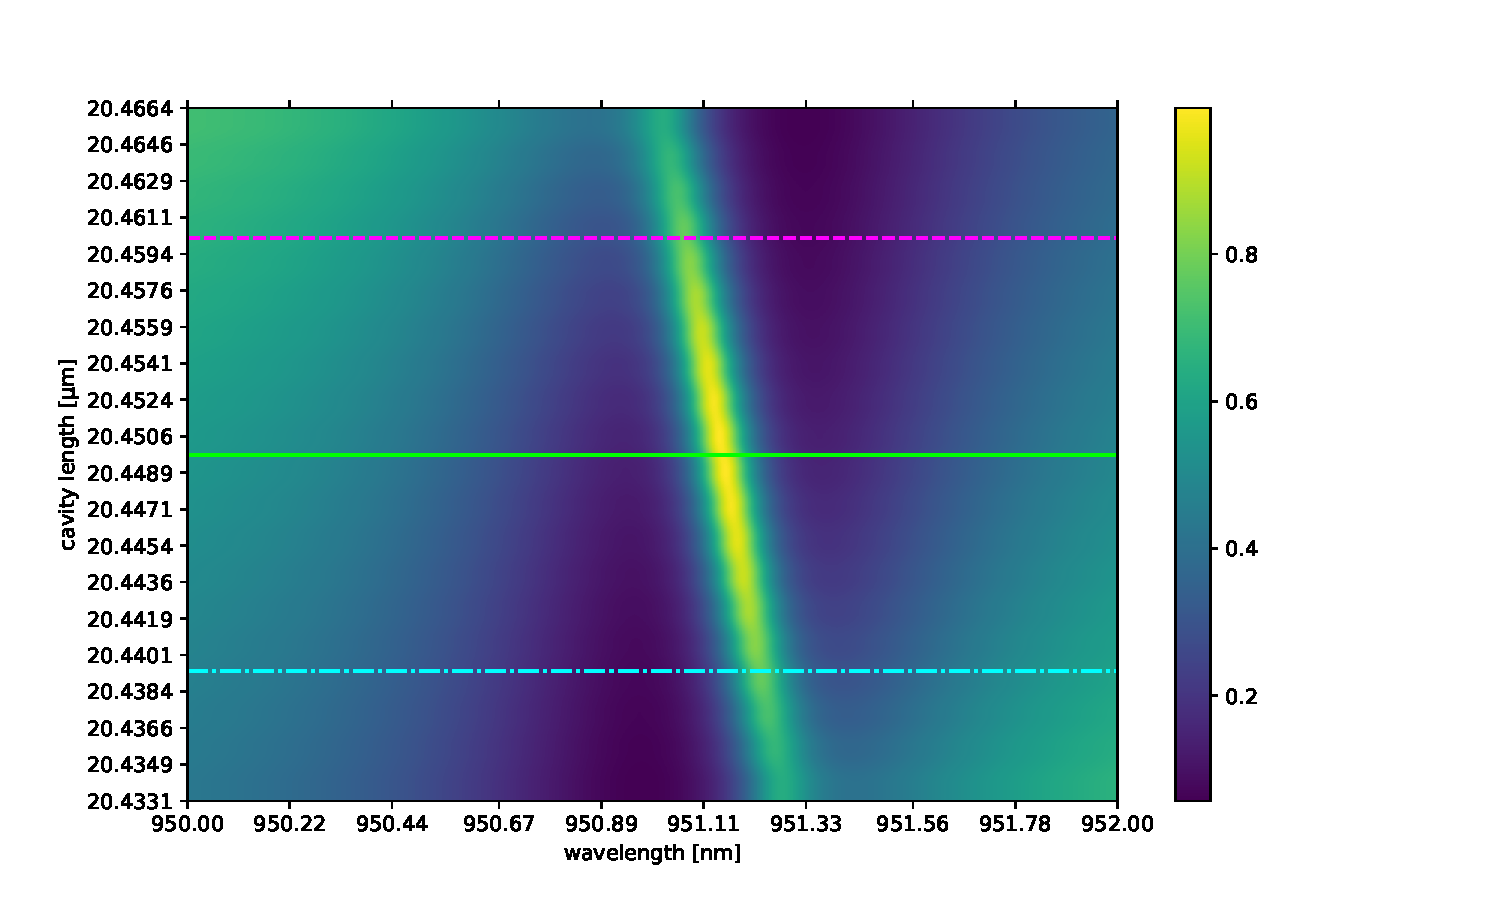
\includegraphics[width=0.7\textwidth]{figures/cmap_with_slice_indicators1.pdf}
    \caption{Heat map of the lossless double Fano cavity transmission as a function of wavelength and cavity lengths ranging $l \rightarrow l^{\prime} \approx 30 \mu m$ for $\Delta = 0.3$nm}
    \label{fig:cmap_single}
\end{figure}

\begin{figure}[h!]
    \centering
    \begin{subfigure}[b]{0.49\textwidth}
        \centering
        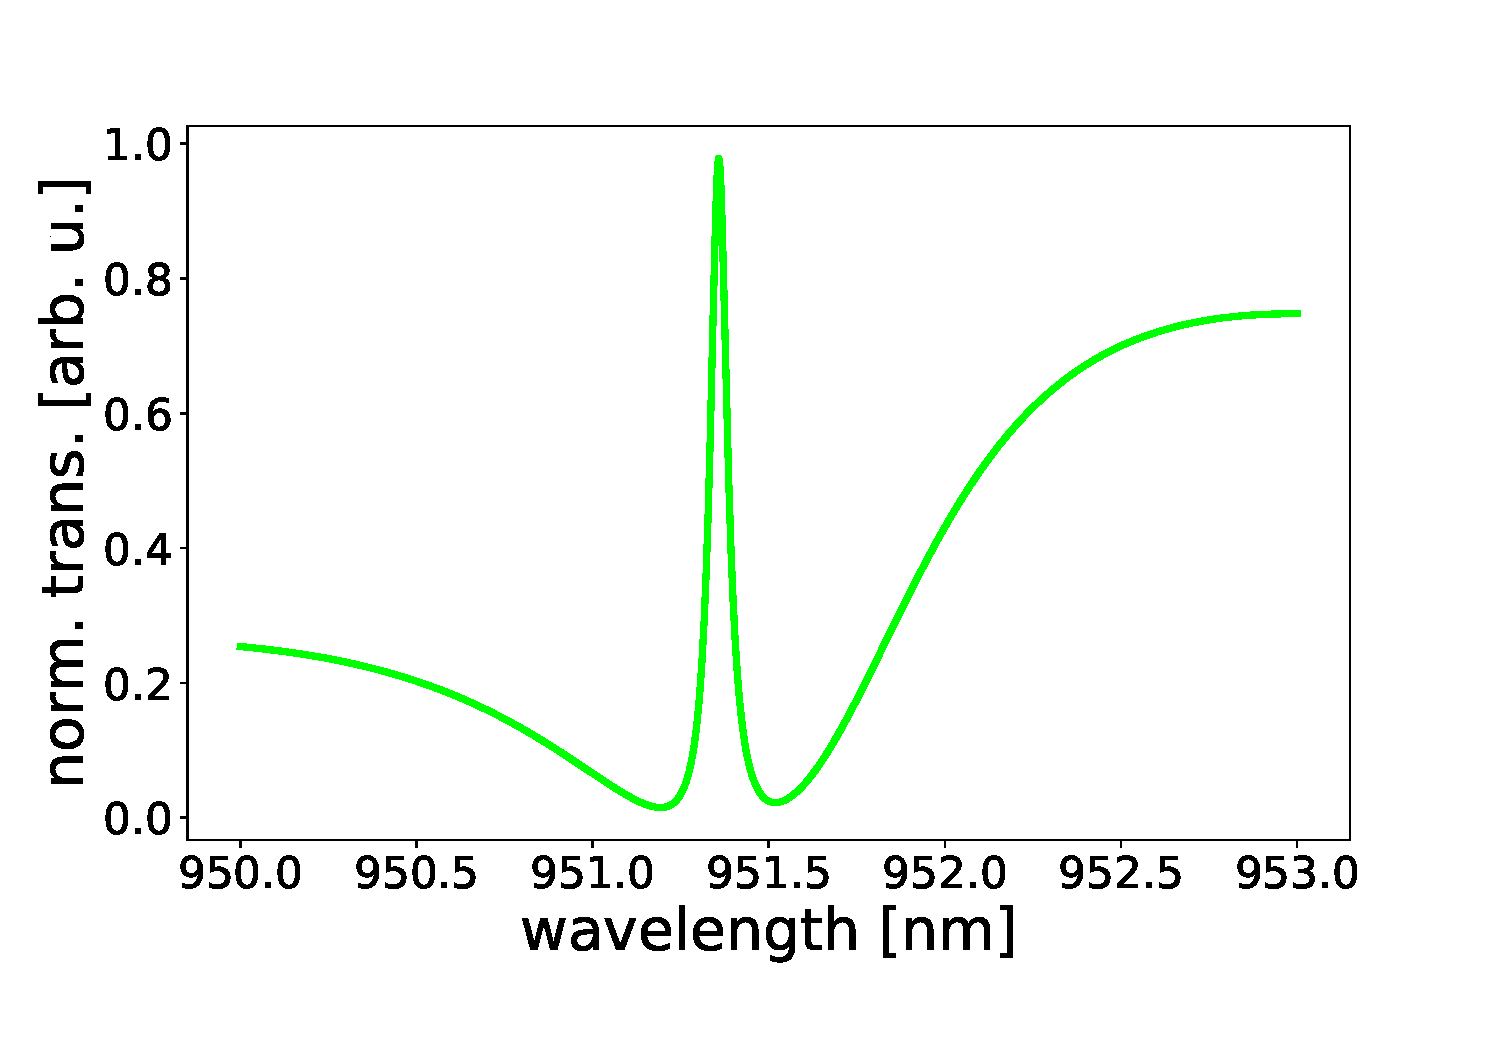
\includegraphics[width=\textwidth]{figures/cmap_slice1.pdf}
        \caption{}
        \label{fig:cmap_slice1}
    \end{subfigure}
    \begin{subfigure}[b]{0.49\textwidth}
        \centering
        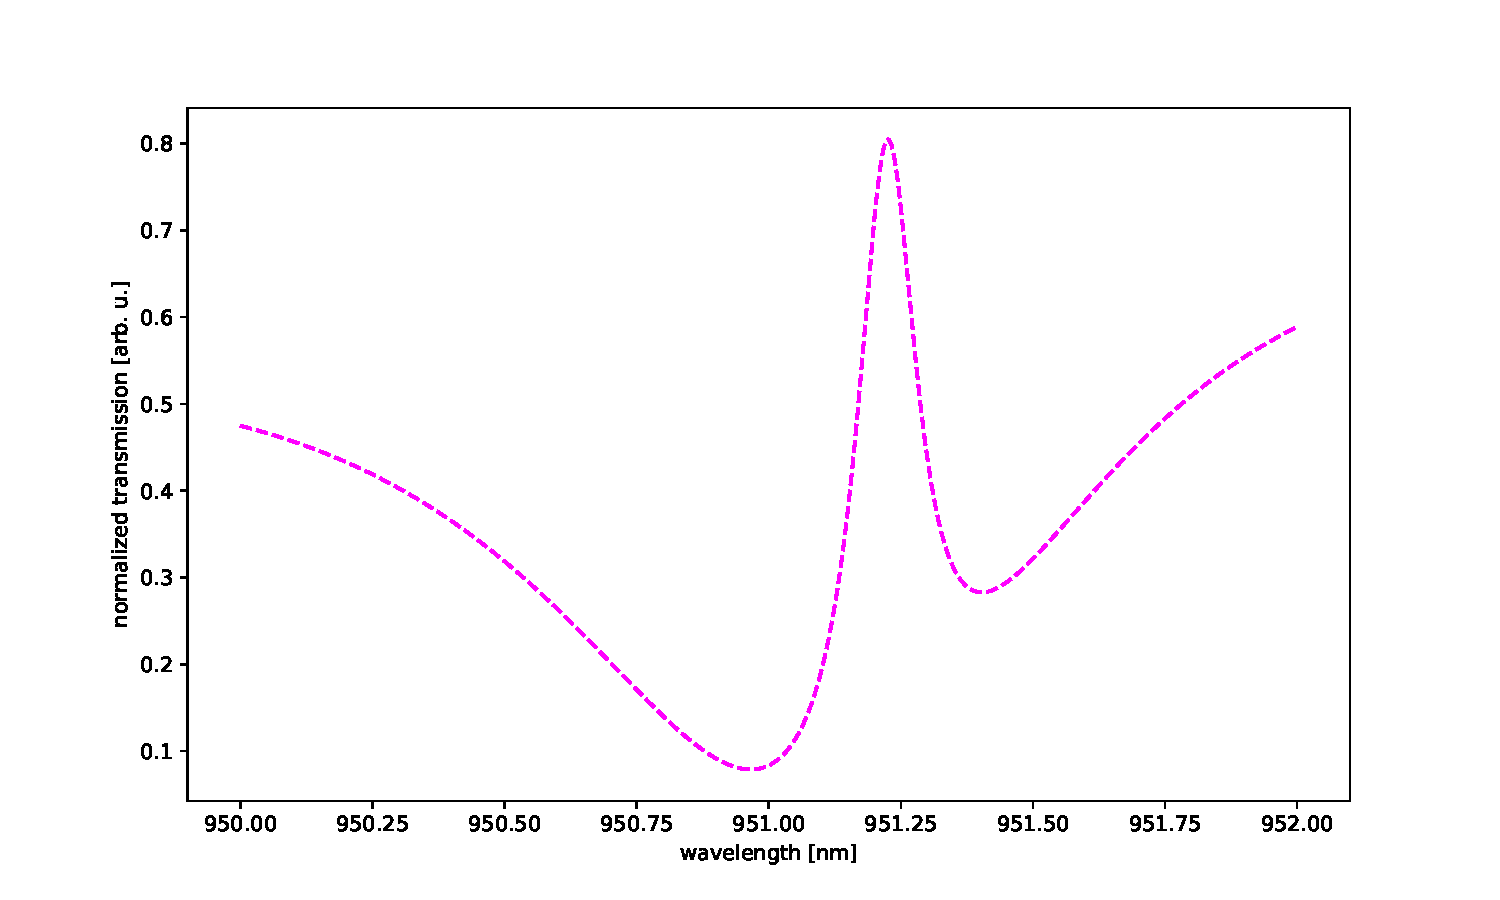
\includegraphics[width=\textwidth]{figures/cmap_slice2.pdf}
        \caption{}
        \label{fig:cmap_slice2}
    \end{subfigure}
    \begin{subfigure}[b]{0.49\textwidth}
        \centering
        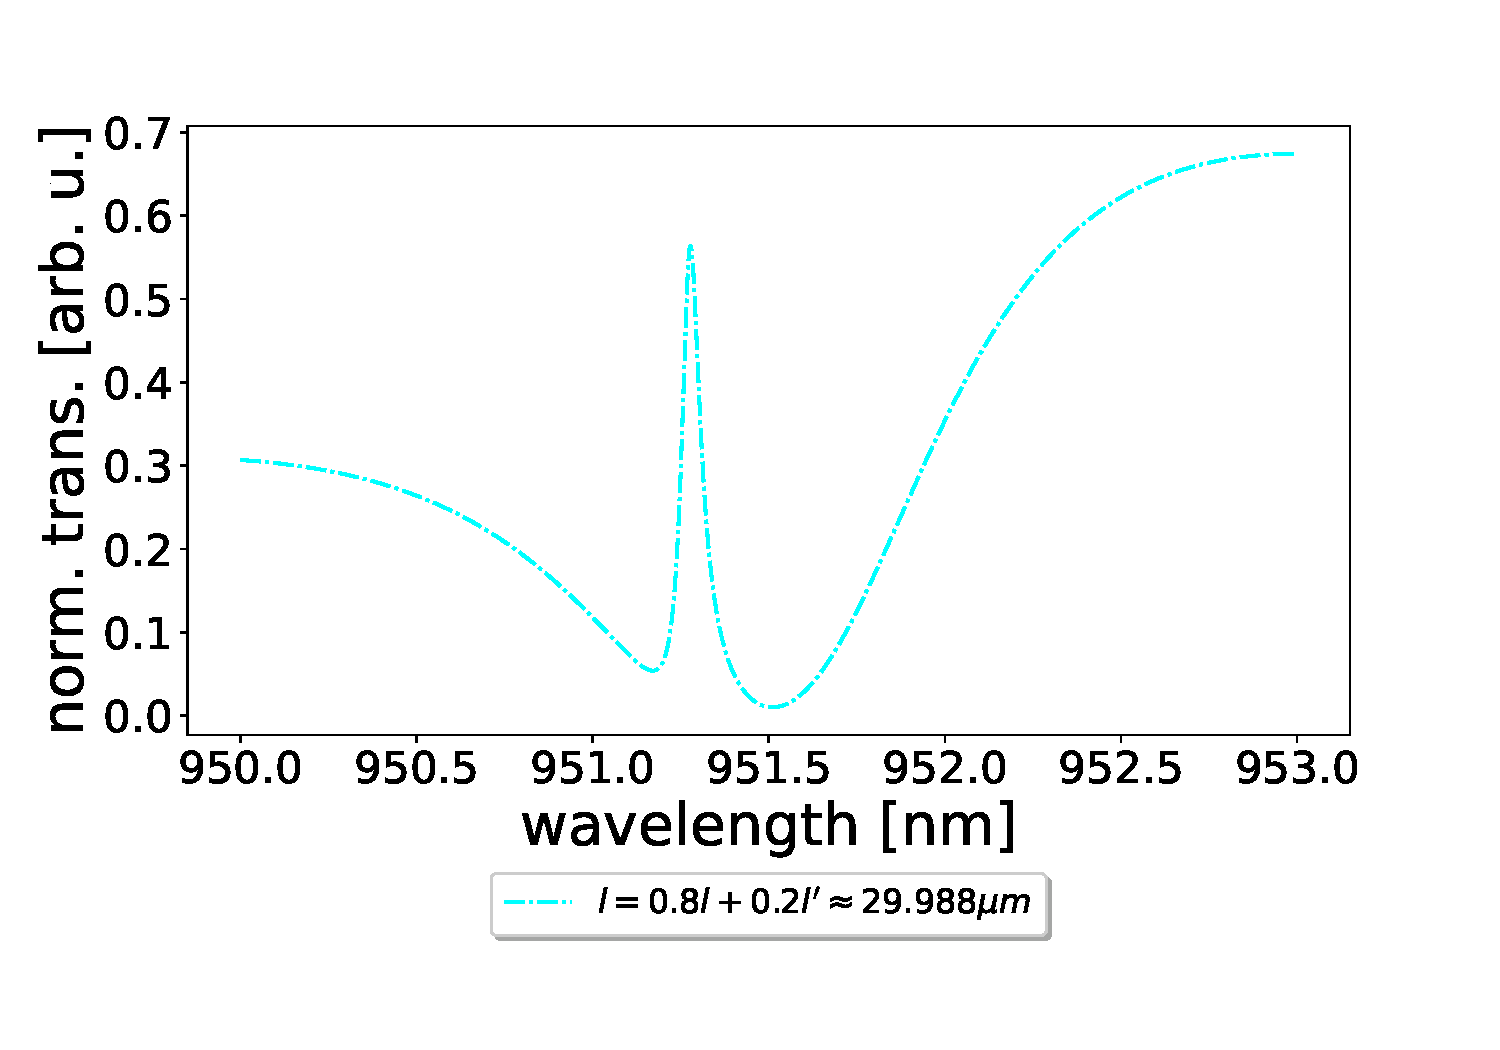
\includegraphics[width=\textwidth]{figures/cmap_slice3.pdf}
        \caption{}
        \label{fig:cmap_slice3}
    \end{subfigure}
    \begin{subfigure}[b]{0.49\textwidth}
        \centering
        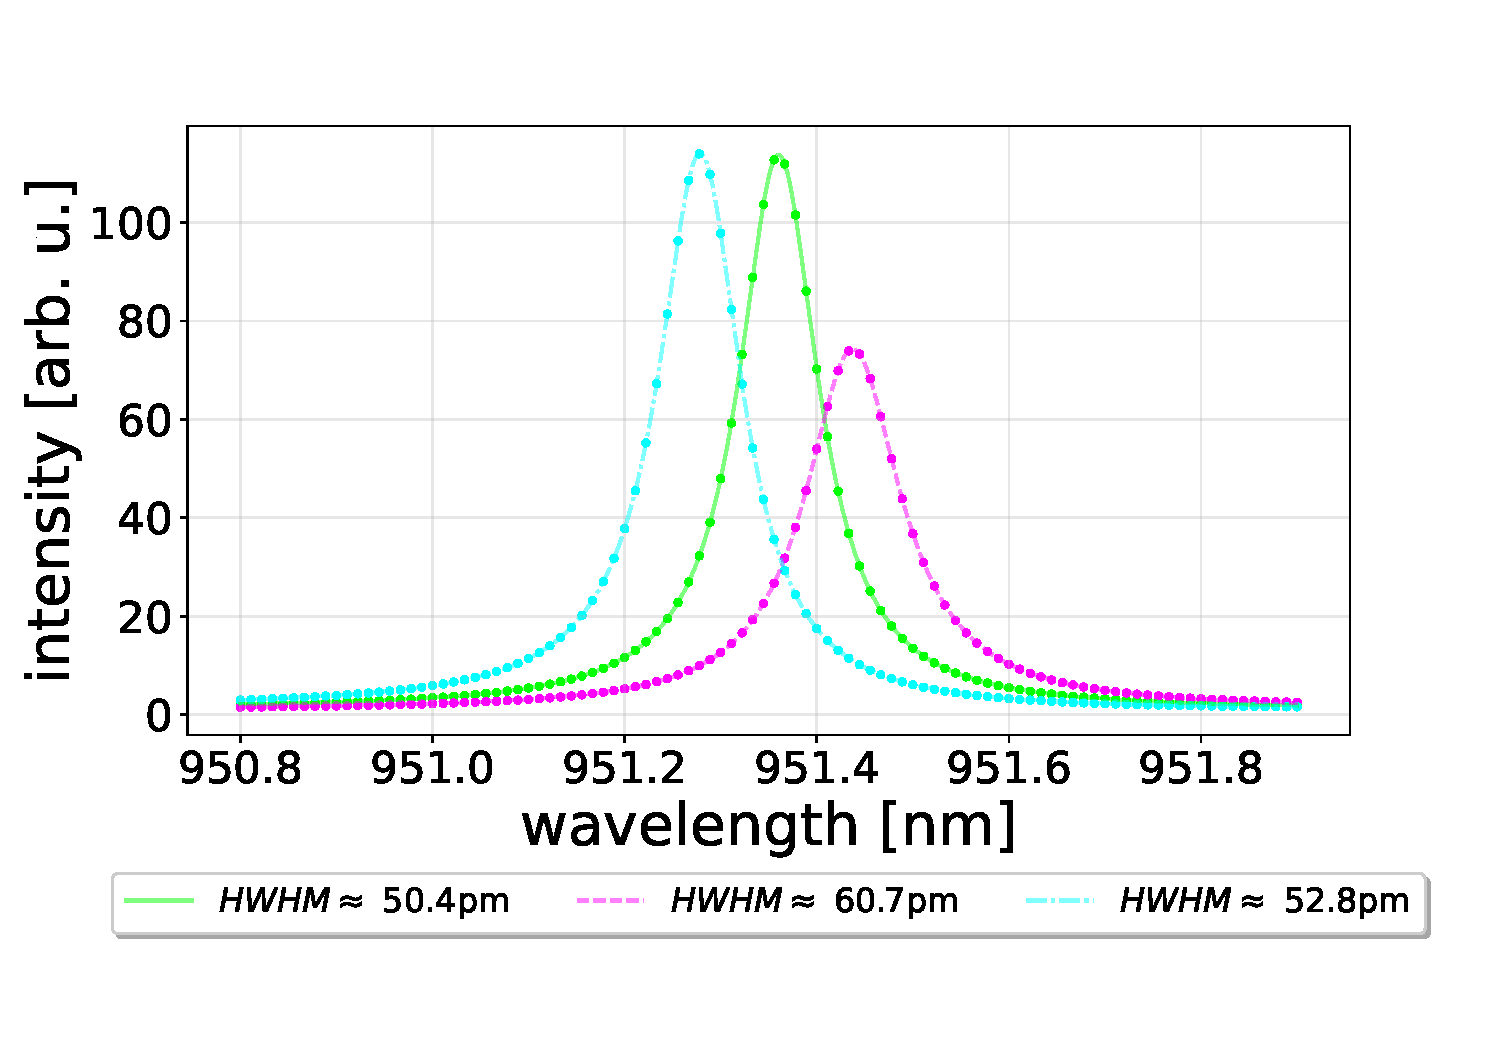
\includegraphics[width=\textwidth]{figures/cmap_lws.pdf}
        \caption{}
        \label{fig:cmap_lws}
    \end{subfigure}
    \caption{(a), (b) and (c) show slices of the heat map in figure \ref{fig:cmap_single} indicated by their respective color an line type in order to compare different cavity lenghts. (d) show intracavity spectra of the peaks in (a), (b) and (c) with corresponding least squares fits and linewidths found as parameters hereof. }
    \label{fig:cmap_slices}
\end{figure}

Considering only the heat map, it is not easily visible which cavity length is the optimal one, however, the \emph{magenta}, \emph{cyan}, and \emph{limegreen} lines across the heat map indicate slices which are depicted separately in figure \ref{fig:cmap_slices}. It is seen by analysing the transmission profiles of the three cavities of specific lengths, how they vary in both position and linewidth. The lengths and corresponding linewidths are given as
\begin{equation}
    \begin{split}
        l_{magenta} = 0.2 l + 0.8 l^{\prime} &\rightarrow HWHM_{magenta} = 40.5pm\\ l_{cyan} = 0.8 l + 0.2 l^{\prime} &\rightarrow HWHM_{cyan} = 31.9pm\\ l_{lime} = (l + l^{\prime})/2 &\rightarrow HWHM_{lime} = 29.7pm.
    \end{split}
\end{equation}
It turns out that of the three cases, the \emph{lime} transmission profile seems optimal as it is the narrowest of the three, and seems to be more preferably positioned, i.e. it is more centered in and thus separated from the Fabry-Perot-like background. 

\begin{figure}[h!]
    \centering
    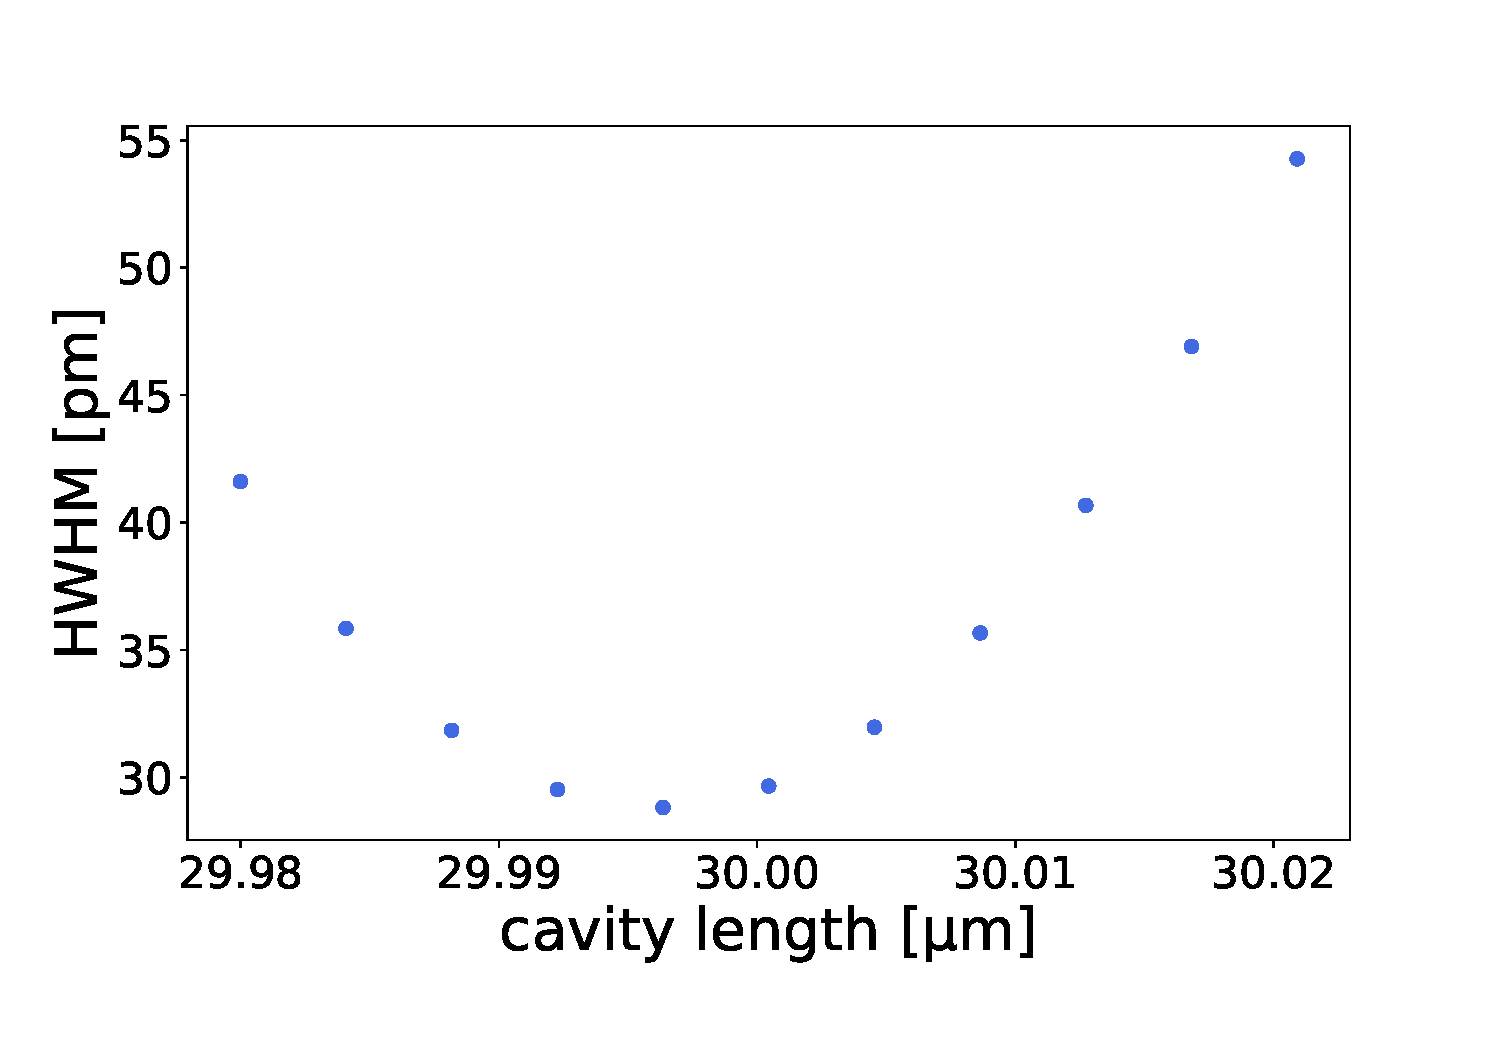
\includegraphics[width=0.7\textwidth]{figures/lw_vs_length_intracavity.pdf}
    \caption{Linewidth as a function of cavity length $l \rightarrow l^{\prime}$. Each point is found as a fitting parameter from a least squares fit to the generalized Fano model in eq. (\ref{eq:general_fano_model}) of lossless intracavity double Fano spectra.}
    \label{fig:lw_vs_l_scan}
\end{figure}

This trend is further examined in figure \ref{fig:lw_vs_l_scan} where the linewidths of intracavity spectra are shown as a function of the cavity length. The parameters used are the same as in figure \ref{fig:cmap_single} and the figure indicates that the optimal cavity length is definitely "somewhere in between" the two guided-,mode resonance lengths. However, it is also evident that the previous assumption for $\lambda_t$ is too simple to be general in this case. 

As a visual and qualitative representation of the effect of increasing the detuning $\Delta$, figure \ref{fig:cmaps_detuning} shows heat maps similar to the one in figure \ref{fig:cmap_single}, but for a range of values for the detuning $\Delta=0.01$nm$ \rightarrow \Delta=1.21$nm. It is readily seen that the aforementioned slope of the high intensity region, indicating the resonance peak, increases with the detuning. This is a representation of the peak moving to higher wavelengths, both for the optimal transmission wavelength and for the one closer to the detuned Fano mirror guided-mode resonance. The broadening of the peak is also displayed in a way that is, while only qualitative, convincing. 

\begin{figure}[h!]
    \centering
    \includegraphics[width=0.95\textwidth]{figures/cmaps_detuning_30um.pdf}
    \caption{Series of heat maps showing lossless double Fano transmission spectra as a function of the cavity length, for increasing detuning $\Delta$.}
    \label{fig:cmaps_detuning}
\end{figure}



\newpage
\section*{Method}
\section{Method}
\subsection{The experimental setup}

The experimental setup used to optically characterize the Fano mirrors, single- and double Fano cavities is illustrated in figure \ref{fig:setup_sketch}. The specific part of the setup surrounding the cavity, outlined by the dashed line in figure \ref{fig:setup_sketch}, is subsequently shown in figure \ref{fig:setup_zoomed}. 

In order to effectively conduct the experiments in this project, it is imperative to be able to control certain parameters. Each element in the experimental setup is thoroughly considered for each their purpose in this regard, these will be outlined in this section. 

\begin{figure}[h!]
    \centering
    \includegraphics[width=0.6\textwidth]{figures/setup_sketch.pdf}
    \caption{Schematics of the experimental setup for measuring Fano cavity transmission- and Fano mirror transmission/reflection spectra. The diode laser \emph{DL} emits light into the setup through the optical fiber, the $\lambda/2$-waveplate \emph{HWP} and polarizing beam splitter \emph{PBS} ensures the light is linearly polarized and the optical telescope consisting of lenses $L_{1,2}$ modifies the beam waist to fit the given purpose. Detectors $P_{T,R,I}$ records the transmitted, reflected and incident light, respectively and the second HWP makes it possible to tune the polarization of the light just before the light is incident on the Fano cavity/mirror. The dashed line indicates the cavity setup seen in detail in figure \ref{fig:cavity_setup}. $I_{1-4}$ and $M_{1-3}$ indicate apertures/iris' and mirrors, respectively.}
    \label{fig:setup_sketch}
\end{figure}

\begin{figure}[h!]
    \centering
    \begin{subfigure}[b]{0.74\textwidth}
        \includegraphics[width=\textwidth]{figures/setup_skecth_zoomed.pdf}
        \caption{}
        \label{fig:setup_zoomed}
    \end{subfigure}
    \begin{subfigure}[b]{0.25\textwidth}
        \includegraphics[width=\textwidth]{figures/setup_cavity_picture.pdf}
        \caption{}
        \label{fig:cavity_setup_picture}
    \end{subfigure}
    \caption{(a) shows a sketch of the schematics of the Fano cavity setup located inside the dashed line in figure \ref{fig:setup_sketch}. The stages attached to both the top and bottom of the cavity are used to spacially align the Fano mirrors of the cavity, while the kinematics mirrors are used to adjust for the angular degrees of freedom. The piezo ring is used to scan for and tune the optimal length of the cavity and the rotational and adjustable xy-mounts are used for aligning the top of the cavity, when the bottom is aligned with respect to the laser, and both are hence fixed. (b) shows a picture of the cavity setup depicted schematically in (a). Note that the setup, both in (a) and (b), depicted is the one used to measure double Fano cavity transmission, and would thus be modified for a Fano mirror characterization.}
    \label{fig:cavity_setup}
\end{figure}

\subsubsection{Tunable diode laser}

As shown in figure \ref{fig:setup_sketch} the laser source used for the optical characterizations is coupled into the setup through an optical fiber. The laser used is a \emph{Toptica DLC Pro} tunable CW diode laser with a range for the transmission wavelength of $910$ $-$ $980nm$. The laser and controller are both depicted in figure \ref{fig:toptica_laser_and_controller}. The optical fiber is a \emph{P3-780PM-FC-10} fiber from Thorlabs which is a single mode\footnote{A single mode fiber can only sustain the TEM00 mode, which means that the output is known to be perfectly Gaussian.} polarization-maintaining optical fiber with an effective range of $770$ $-$ $1100nm$. Between the Toptica laser and the incoupling end of the fiber, a $\lambda/2$\emph{-plate} (HWP) and \emph{polarizing beam splitter} (PBS) is placed in order to be able to control the incident power of the laser and to only couple linearly polarized light into the setup.  

\begin{figure}[h!]
    \begin{subfigure}[b]{0.49\textwidth}
        \centering
        \includegraphics[height=4cm]{figures/toptica_laser.pdf}
        \caption{}
        \label{fig:toptica_laser}
    \end{subfigure}
    \begin{subfigure}[b]{0.49\textwidth}
        \centering
        \includegraphics[height=4cm]{figures/toptica_controller.pdf}
        \caption{}
        \label{fig:toptica_controller}
    \end{subfigure}
    \caption{The Toptica DLC Pro tunable CW diode laser (a) and the controller (b) used to tune the wavelength of the output beam.}
    \label{fig:toptica_laser_and_controller}
\end{figure}

The light being emitted from the optical fiber is sent through another HWP and PBS in order to be able to control the resulting polarization in the setup even more precisely, should there be any discrepancies of the light coupled into the fiber. The out-coupling fiber with the HWP and PBS is shown in figure \ref{fig:outcoupling_fiber}.

\begin{figure}[h!]
    \centering
    \includegraphics[width=0.5\textwidth]{figures/outcoupling_fiber.pdf}
    \caption{The out-coupling end of the P3-780PM-FC-10 polarization maintaining optical fiber from Thorlabs along with the HWP and PBS ensuring linear polarizaed light incident on the cavity or Fano mirror.}
    \label{fig:outcoupling_fiber}
\end{figure}

\subsubsection{$\lambda / 2$ - waveplate}

A $\lambda/2$-waveplate, or HWP, is constructed of a so-called bi-refringent material (most commonly crystaline quartz), which means that it has slightly different refractive indicies for incident light of different polarization axis'. Generally a HWP will have a \emph{fast}- and \emph{slow axis}, where it is understood that light polarized along the fast axis experiences a lower refractive index (and hence moves faster), than that along the slow axis. In this way the HWP separates the components of unpolarized light that has perpendicular and parallel polarizations with respect to the fast axis. 

\begin{figure}[h!]
    \centering
    \includegraphics[width=0.6\textwidth]{figures/HWP.pdf}
    \caption{A simple sketch of the effect of a HWP on linearly polarized light.}
    \label{fig:HWP}
\end{figure}

The effect of the HWP on linearly polarized light, is an effective rotation of the polarization, this is sketched simply in figure \ref{fig:HWP}. It can be shown that the polarization axis is rotated according to the angle between the fast axis of the HWP and the incident polarization axis. A relative angle $\theta$ will thus result in a rotation of $2\theta$, e.g. if $\theta=45^{\circ}$, this will constitute a rotation from completely p-polarized light to completely s-polarized light. This is the specific scenario sketched in figure \ref{fig:HWP}\cite{edmund_optics}. In this way a rotating HWP can allow one to alter an incident linearly polarized beam to be polarized along any axis, and is thus a necessary component for this particular setup.

\subsubsection{Optical telescope}

The linearly polarized light transmitted through the PBS passes through plano-convex lenses of positive focal lengths $f$ and $f^{\prime}$, $L_1$ and $L_2$, which together makes up an optical telescope used to manipulate the beam waist $w_0$ incident on the cavity or Fano mirror. 

Figure \ref{fig:telescope} shows schematics of the general way an optical telescope is utilized to manipulate the beam waist of a laser beam.

\begin{figure}[h!]
    \begin{subfigure}[b]{0.49\textwidth}
        \centering
        \includegraphics[height=4cm]{figures/optical_telescope.pdf}
        \caption{}
        \label{fig:telescope}
    \end{subfigure}
    \begin{subfigure}[b]{0.49\textwidth}
        \centering
        \includegraphics[height=4cm]{figures/optical_telescope_picture.pdf}
        \caption{}
        \label{fig:telescope_picture}
    \end{subfigure}
    \caption{(a) shows simple schematics of an optical telescope used to alter the waist of an incomming collimated beam, while (b) shows a picture taken of the actual optical telecope used in the setup.}
    \label{fig:telescope_sketch_and_pic}
\end{figure}

When the incident beam hits $L_1$ it is focused according to its focal length $f$, and by inserting another lens $L_2$ of a relatively longer focal length one can \emph{catch} the beam at the desired beam waist. If the focal length $f^{\prime}$ of $L_2$ is sufficently long, compared to the path of the beam after the lenses, the beam will be approximately collimated and remain at the waist obtained when incident on $L_2$.

\subsubsection{Transmission, reflection and incident photo-detectors}

After passing the optical telescope the beam reaches a simple 50/50 beam splitter (BS) which transmits 50\% of the light while reflecting another 50\%. The reflected light is then incident on the cavity or Fano mirror (target). 

The transmitted light passes through a lens $L_3$, which is focused on a photo-detector $P_I$ used for reference measurements and later normalization. Since the tunable laser in nature varies in power with the wavelength, it is necesarry to keep track of these fluctuations and correct for them in data analysis. 

The transmitted light is sent through, yet another, HWP which in this case is used only to alter the polarization of the light incident on the target. After the beam, or a portion of it, has passed the target it is sent through a lens $L_5$ focused onto the transmission detector $P_T$.

The part of the light incident on the target that is \emph{not} transmitted, is reflected back onto the BS which then transmits 50\% once again, and thus reflects the other 50\%. The transmitted part here is focused through the lens $L_4$ onto the reflection detector $P_R$.

\subsubsection{The double Fano cavity measurement setup}

The cavity measurement setup shown in figure \ref{fig:setup_zoomed} is the one used to measure the transmission spectrum of a double Fano cavity consisting of two Fano mirrors. This part of the setup consists of two sets of standard \emph{PT1} $\mu m$-stages from Thorlabs combined to provide precise movement of each Fano mirror in the xy-plane. 

\begin{figure}[h!]
    \centering
    \begin{subfigure}[b]{0.6\textwidth}
        \includegraphics[width=\textwidth]{figures/setup_bottom.pdf}
        \caption{}
        \label{fig:setup_bottom}
    \end{subfigure}
    \begin{subfigure}[b]{0.3\textwidth}
        \includegraphics[width=\textwidth]{figures/cavity_setup_bottom_pic.pdf}
        \caption{}
        \label{fig:setup_bottom_pic}
    \end{subfigure}
    \caption{(b) shows a picture taken of the \emph{bottom} part of the double Fano cavity setup, while (a) depicts the corresponding schematics.}
    \label{fig:setup_bottom_sketch_and_pic}
\end{figure}

Examining the structure from the bottom (as it is built), a kinematic mirror mount is attached to the lower set of xy-stages, this is used to control the angular degrees of freedom of the Fano mirror which makes up the bottom of the cavity. On the mirror mount, a \emph{NAC2123} piezo ring actuator from Noliac is firmly attached and connected to a piezo driver. The driver is capable of applying a fixed current, and thus manually controlling the piezo expansion, but is also connected to a frequency generator. The signal from the frequency generator can be used to modulate the piezo expansion by an alternating current, which practically scans the cavity length in a range according to the effective free stroke of the piezo ring\footnote{The NAC2123 piezo ring has an outer/inner diameter of $12mm/6mm$ and a height of $2mm$. Its listed free stroke is $3.3 \mu m$, which practically is likely slightly limited in the configuration used. To obtain the precise free stroke one can simply count the number of fringes resolved during one period as the length-dependent FSR is known to be $\lambda/2$.}. Lastly, in order to be able to place the Fano mirror on the  piezo ring, a ceramic Macor membrane holder is used. The bottom part of the cavity setup is highlighted in figure \ref{fig:setup_bottom}.

The part of the setup built to control the Fano mirror making up the top of the cavity is slightly more complicated, as this is the Fano mirror that is, for practical reasons, aligned last. This means that additional degrees of freedom must be controled by movement of the Fano mirror itself. The alignment procedure will be explained in detail in sections \ref{sec:grating_characterization} and \ref{sec:cavity_measurements}.

\begin{figure}[h!]
    \centering
    \begin{subfigure}[b]{0.6\textwidth}
        \includegraphics[width=\textwidth]{figures/setup_top.pdf}
        \caption{}
        \label{fig:setup_top}
    \end{subfigure}
    \begin{subfigure}[b]{0.3\textwidth}
        \includegraphics[width=\textwidth]{figures/setup_top_pic.pdf}
        \caption{}
        \label{fig:setup_top_pic}
    \end{subfigure}
    \caption{(b) shows a picture taken of the \emph{top} part of the double Fano cavity setup, while (a) depicts the corresponding schematics.}
    \label{fig:setup_top_sketch_and_pic}
\end{figure} 

The top part of the cavity setup is attached to the second set of xy-stages and additionally to an \emph{NFL5DP20} stage from Thorlabs in the z-direction in order to be able to change the length of the cavity. As for the bottom part of the cavity setup, a kinematic mirror mount acts as the base of the construction. This is, once again, to control the angular degrees of freedom of the corresponding Fano mirror. This mirror mount is equipped with piezo elements to control the angular degrees of freedom, by applied voltage, with higher resolution than for the manual adjustments. On the mirror mount, a standard rotational mount with a 1 inch inner winding is attached in order to be able to control the rotational degree of freedom of the Fano mirror. An additional xy-adjustable mount is then used in order to effectively place the Fano mirror in the center of the rotational mount to ensure the rotational axis is in the center of the membrane. Finally, the Fano mirror is taped to a costume mount created to fit into the xy-adjustable mount. The top part of the cavity setup is highlighted in figure \ref{fig:setup_top}, and presented separate from the setup to show how the Fano mirror is attached in figure \ref{fig:cavity_setup_top_separate_pic}.

\begin{figure}[h!]
    \centering
    \includegraphics[width=0.4\textwidth]{figures/cavity_setup_top_separate_pic.pdf}
    \caption{The top part of the cavity setup separated from the rest and flipped. Note that the Fano mirror attached with the tape is shown. The three wires visible are then ones that connect the piezo elemehts with a driver.}
    \label{fig:cavity_setup_top_separate_pic}    
\end{figure}

What has been outlined here is the setup utilized to optically characterize the double Fano cavity. If one wishes to do so for the single Fano cavity instead, the setup would be modified such that the top part of the setup, highlighted in figure \ref{fig:setup_top}, would only consist of the kinematic mirror mount. Inside the mirror mount would then be placed a broadband mirror. The rotational- and xy-adjustable mounts would here be redundant due to the rotational symmetry of any standard broadband mirror.

\subsubsection{Acoustic noise reduction}

When the cavity measurements were conducted it was apparent that the double Fano cavity was particularly prone to noise. While noise is not a very precise definition in its own, it did seem that the most prominent source was associated with the length of the cavity $l$. When applying a constant voltage to the piezo element depicted in figure \ref{fig:setup_bottom_sketch_and_pic}, in order to achieve the correct length for sustaining the Fano resonance, the level started to fluctuate dramatically when approaching the resonance. 

\begin{figure}[h!]
    \centering
    \begin{subfigure}[b]{0.49\textwidth}
        \centering
        \includegraphics[height=4.5cm]{figures/noise_box_front.pdf}
        \caption{}
        \label{fig:box_front}
    \end{subfigure}
    \begin{subfigure}[b]{0.49\textwidth}
        \centering
        \includegraphics[height=4.5cm]{figures/noise_box_side.pdf}
        \caption{}
        \label{fig:box_side}
    \end{subfigure}
    \caption{Front- (a) and side (b) views of the plexi-glass box used to reduce the acoustic noise in the setup.}
    \label{fig:noise_box}
\end{figure}

By examining the characteristics of the noise when apparent, the source appeared to be acoustic in origin, i.e. making a sudden sound in close vicinity of the setup caused a spike in the noise level.

In order to reduce the acoustic noise, a plexi-glas box was placed around the entire setup as seen in figure \ref{fig:noise_box}. This proved to reduce the noise, and this improve the signal-to-noise, ratio substantially.

\subsubsection{Additional equipment used}

In order to record a measurement of any kind in the setup, a \emph{Keysight InfiniiVision DSOX2024A} oscilloscope was connected with all the detectors $P_T$, $P_R$ and $P_I$ in the setup. The oscilloscope, along with the Toptica laser, was then controlled by a Matlab script implemented by previous students/researchers of the lab. 

Scanning the piezo element, by application of an altertnating current also required additional equipment, and more specifically a frequency generator capable of generating a triangular signal with an offset. The frequency generator used was a \emph{Keysight 33500B Waveform Generator}. Insight on scanning the cavity length using the piezo will be provided in section \ref{sec:cavity_measurements}. The oscilloscope and frequency generater are shown in figure \ref{fig:scope_and_freq_generator}.

\begin{figure}[h!]
    \centering
    \begin{subfigure}[b]{0.49\textwidth}
        \centering
        \includegraphics[height=4cm]{figures/scope.pdf}
        \caption{}
        \label{fig:scope}
    \end{subfigure}
    \begin{subfigure}[b]{0.49\textwidth}
        \centering
        \includegraphics[height=4cm]{figures/frequency_generator.pdf}
        \caption{}
        \label{fig:freq_generator}
    \end{subfigure}
    \caption{Pictures of the oscilloscope (a) and frequency generator (b) used during experimental investigations in this project.}
    \label{fig:scope_and_freq_generator}
\end{figure}


\newpage
\section*{Results}
\section{Simulations}

Figures:
\begin{itemize}
    \item Simulated spectra of M3 and M5.
    \item Simulated length scans of M3 and M5.
    \item M3/M5 cavity trans. spectra (on resonance + full range)
    \subitem for lengths: $l_{M3} \rightarrow l_{M5}$
    \subitem for length: $l = 1/2 \cdot (l_{M3} + l_{M5})$
    \item Optimal result comparison with single fano/broadband cavities of similar losses.
    \item Optimal result comparison with the ideal case from prev. section.
    \item Simulated linewidth as a function of cavity length (include the same for broadband and single fano cavities).
\end{itemize}
\newpage
\section{Results}

The aim of this project has been to realize the double Fano cavity experimentally and investigate its transmission profile as a function of the incident wavelength. In this section I present the best results obtained and comment on these. Furthermore, I will outline challenges and obstacles that have been encountered, their implications on the data presented and my thoughts on immediate improvements for future experiments. 

The results obtained have been so through an iterative process realizing the theory presented in previous sections. For this reason, the structure of this section will outline this process and thus begin by an in depth spectral analysis of the Fano mirrors used, as a pair matching in optical parameters, and especially the guided-mode resonance wavelength, is crucial in order to realize the Fano resonance. When moving on to the results regarding cavity characterization I will begin by briefly verifying the results for the single Fano cavity presented by Mitra et al. in \cite{Mitra}. Finally, I will show experiemental results of the optical characterization of the double Fano cavity. 

\subsection{Fano mirror characterization}\label{sec:results_fano_mirror_characterization}

The first important step in realizing the double Fano cavity, is to locate a matching pair of Fano mirrors. A substantial spectral overlap is necessary in order to excite a Fano resonance including both guided-modes, as explained in section \ref{sec:spectral_detuning}. For this reason the Fano mirrors considered were all fabricated externally by \emph{Norcada} and from the same "batch", as these were initially considered to have a greater probability of having similar physical attributes. Many Fano mirrors were thus characterized during the process of finding a match, and the pair eventually chosen to move forward with were denoted \emph{G1} and \emph{G2}. 

\begin{figure}[h!]
    \centering
    \begin{subfigure}[b]{0.49\textwidth}
        \includegraphics[width=\textwidth]{figures/results/M3:M5/M5:G1_initial_spectrum.pdf}
        \caption{}
        \label{}
    \end{subfigure}
    \begin{subfigure}[b]{0.49\textwidth}
        \includegraphics[width=\textwidth]{figures/results/M3:M5/M3:G2_initial_spectrum.pdf}
        \caption{}
        \label{}
    \end{subfigure}
    \caption{(a) shows the normalized reflection and transmission spectra of Fano mirror G1 along with its optical parameters found as fitting parameters from a least squares fit to the model derived in section \ref{sec:fano_mirror}. (b) shows the same for Fano mirror G2. Spectra of Fano mirrors that were characterized but not included in further experiments can be found in Appendix \ref{appendix:Additional Fano mirror characterizations}.}
    \label{fig:individual_G1_and_G2_spectra}
\end{figure}

Figure \ref{fig:individual_G1_and_G2_spectra} shows the individual measured normalized reflection and transmission spectra of G1 and G2 together with a least squares fit to the model derived in section \ref{sec:fano_mirror}. The corresponding optical parameters for each Fano mirror were found as the following.

Fitting parameters for G1:
\begin{equation}
    \begin{split}
        \lambda_{0,G1} &= 951.764 \text{nm}, \:\: \lambda_{1,G1} = 951.901 \text{nm},\:\: t_d = 0.814, \\&r_d = 0.575, \:\:  \gamma_{\lambda} = 0.462 \text{nm},\:\: \beta = 9 \cdot 10^{-7} \text{nm}^{-1}.
    \end{split}
    \label{eq:G1_params}
\end{equation}

Fitting parameters for G2:
\begin{equation}
    \begin{split}
        \lambda_{0,G2} &= 951.855 \text{nm}, \:\: \lambda_{1,G2} = 951.997 \text{nm},\:\: t_d = 0.814, \\&r_d = 0.570, \:\:  \gamma_{\lambda} = 0.482 \text{nm},\:\: \beta = 1 \cdot 10^{-6} \text{nm}^{-1}.
    \end{split}
    \label{eq:G2_params}
\end{equation}

In order to evaluate and compare the parameters to determine whether the two Fano mirrors are in fact a good match, they are both shown alongside eachother in figure \ref{fig:G1_and_G2_spectral_comparison} for spectral comparison. Each their resonance wavelengths $\lambda_0$ are indicated on the figure and the detuning can thus be estimated as 
\begin{equation}
    \Delta = \left|\lambda_{0,G2} - \lambda_{0,G1}\right| = 951.855 \text{nm} - 951.764 \text{nm} = 0.091 \text{nm}.
    \label{eq:G1/G2_detuning}
\end{equation}

Here we remember that the additional fitting parameters, namely $t_d$, $r_d$, $\gamma_{\lambda}$ and $\beta$, are assumed identical in the model for the double Fano cavity outlined in section \ref{sec:double_fano_lw_theory} and these are thus compared in a more qualitative manner. Whether the parameters in eqs. (\ref{eq:G1_params}) and (\ref{eq:G2_params}) can be assumed identical is completely individual to the given experiment and the corresponding acceptable margins. In order to move forward, G1 and G2 are assumed to only differ in guided-mode resonance wavelength.

\begin{figure}[h!]
    \centering
    \includegraphics[width=0.7\textwidth]{figures/results/M3:M5/M3:M5_initial_spectra.pdf}
    \caption{Spectral comparison of Fano mirrors G1 and G2. The spectra are the same shown in figure \ref{fig:individual_G1_and_G2_spectra}.}
    \label{fig:G1_and_G2_spectral_comparison}
\end{figure}

As is shown in section \ref{sec:spacial_detuning}, a spectral detuning leads to a spatial detuning, meaning that the cavity length corresponding to the guided-mode resonance wavelength for G1 and G2 are not identical as they have a non-zero detuning $\Delta$. In order to sustain a Fano resonance it is equally important, and in fact equivalent to the spectral overlap, that the Fano mirrors have overlapping cavity transmission profiles as a function of the cavity length. Figure \ref{fig:G1/G2_length_scan} shows the simulated double Fano transmission of a cavity consisting of G1 and G2 for lengths corresponding to their guided-mode resonance wavelengths. It is readily seen that the two transmission profiles overlap for the included example of a cavity of length $l \approx 30 \mu m$.

\begin{figure}[h!]
    \centering
    \includegraphics[width=0.7\textwidth]{figures/results/M3:M5_length_scan_sim_30um.pdf}
    \caption{Simulated length scans of double Fano cavities with incident wavelengths of $\lambda_{0,G1}$ and $\lambda_{0,G2}$. The cooresponding lengths determined from the scans are denoted $l_{G1}$ and $l_{G2}$, respectively.}
    \label{fig:G1/G2_length_scan}
\end{figure}

\clearpage
\subsection{The single Fano cavity}\label{sec:the_single_fano_cavity_results}

We recall that the single fano cavity consists of a Fano mirror and a broadband mirror in a plane-plane configurations where each mirror is perpendicular to the optical axis. The single Fano cavity configuration is briefly outlined in section \ref{sec:cavity_measurements} and otherwise shown in \cite{Mitra}, it however resembles the double Fano cavity setup shown in figure \ref{fig:cavity_setup}, except only the bottom two xy-stages are used, and the top ones are therefore removed.   

The mirror used is a high relfective (HR) broadband mirror with a reflectivity of $99.7\%$, meaning that effectively all intrinsic cavity losses can be assumed to be associated with the Fano mirror. The Fano mirror used is G1 characterized in section \ref{sec:results_fano_mirror_characterization}. 

Figure \ref{fig:single_fano_fsr_scans} shows examples of off-resonance spectra of the single Fano cavity, with corresponding fits to the Fabry-Perot transmission function, in order to determine the cavity length from the measured FSR. Figure \ref{fig:short_single_fano_FSR} shows the off-resonance spectrum for a cavity of length $l = 57.40 \pm 1.55 \mu m$, while figure \ref{fig:long_single_fano_FSR} shows the same for a cavity length of $l = 211.98 \pm 3.16 \mu m$. The errors are determined as the errors of the fit, found as the squareroot of the diagonal of the corresponding covariance matrices.

\begin{figure}[h!]
    \centering
    \begin{subfigure}[b]{0.49\textwidth}
        \centering
        \includegraphics[width=\textwidth]{figures/results/single fano fits/60um_off_res_fabry_perot.pdf}
        \caption{}
        \label{fig:short_single_fano_FSR}
    \end{subfigure}
    \begin{subfigure}[b]{0.49\textwidth}
        \centering
        \includegraphics[width=\textwidth]{figures/results/single fano fits/220um_off_res_fabry_perot.pdf}
        \caption{}
        \label{fig:long_single_fano_FSR}
    \end{subfigure}
    \caption{(a) shows an off-resonance wavelength scan of single Fano cavity consisting of a HR broadband mirror and G1 for a cavity length of $l = 57.40 \pm 1.55 \mu m$. (b) shows this for a single Fano cavity of length $l = 211.98 \pm 3.16 \mu m$. Each length is determined from these measurements by measuring the FSR and utilizing that $l = \lambda_0^2/(2\cdot FSR)$.}
    \label{fig:single_fano_fsr_scans}
\end{figure}

Figure \ref{fig:M5/G1_single_fano_trans_examples} shows examples of resonance transmission spectra of the single Fano cavity. The examples are taken for lengths corresponding to the ones found from the off-resonance spectra shown in figure \ref{fig:single_fano_fsr_scans} above. The figures are depicted with each their corresponding least squares fits to the generalized Fano model shown in eq. (\ref{eq:general_fano_model}) in order to determine the linewidth (HWHM) of the profile. The errors of the linewidths are here found from the error of the fit and are mainly used to determine the quality of the measurement. 

\begin{figure}[h!]
    \centering
    \begin{subfigure}[b]{0.49\textwidth}
        \centering
        \includegraphics[width=\textwidth]{figures/results/single fano fits/60um_M5_fit_1.pdf}
        \caption{}
        \label{fig:short_single_fano_trans}
    \end{subfigure}
    \begin{subfigure}[b]{0.49\textwidth}
        \centering
        \includegraphics[width=\textwidth]{figures/results/single fano fits/220um_M5_fit_4.pdf}
        \caption{}
        \label{fig:long_single_fano_trans}
    \end{subfigure}
    \caption{Single Fano resonance transmission profiles of a cavity consisting of a HR broadband mirror of reflectvitiy $R=99.7\%$ and Fano mirror G1. (a) shows the profile of a cavity of length $l = 57.40 \pm 1.55 \mu m$ and displays a linewidth of $HWHM = 33.907 \pm 3.838$pm. (b) shows the profile of a cavity of length $l = 211.98 \pm 3.16 \mu m$, with a linewidth of $HWHM = 11.982 \pm 0.964$pm.}
    \label{fig:M5/G1_single_fano_trans_examples}
\end{figure}

At each cavity length, the resonance transmission profile was recorded a number of times and the average value was taken to be the true found value of the linewidth. Figure \ref{fig:HWHM_vs_length_single_fano_data} shows the result of a measurement series consisting of five cavity lengths approximately ranging from $20\mu m \leq l \leq 400 \mu m$, where the error of each measurement is given as the standard deviation of the values of all measurements recorded at each cavity length\cite{Hughes}. The error depicted in the x-direction is found from the error of the fit of the Fabry-Perot transmission function to the off-resonance spectra. The blue dashed line indicates the linewidth of a broadband cavity of similar losses according to eq. (\ref{eq:analytical_linewidth_broadband}) and the orange dashed line indicates the analytical linewidth of the single Fano cavity considered consisting of G1 and the HR broadband mirror estimated using eq. (\ref{eq:analytical_linewidth_single_fano}). The black points are linewidths found by fitting single Fano transmission profiles simulated using eq. (\ref{eq:single_fano_trans}) to the generalized Fano model in eq. (\ref{eq:general_fano_model}) for comparison. 

It is seen that the analytical model, the simulated linewidths and the measured linewidths coincide very well for the cavity lengths that are well-within the Fano regime and deviates slightly for longer lengths. This trend agrees nicely with what has previously been found for the single Fano cavity transmission\cite{Mitra} and is likely a consequence of the very narrow linewidths of the cavity in the standard regime, as this increases the sensitivity to any noise regarding the cavity length, e.g. mechanical vibrations in the setup.

\begin{figure}[h!]
    \centering
    \includegraphics[width=0.7\textwidth]{figures/results/HWHM_vs_cavity_length_single_fano.pdf}
    \caption{The linewidth (HWHM) as a function of resonant cavity length. The blue dashed line indicates the analytical linewidth for a broadband cavity, and the orange dashed line shows the corresponding analytical linewidth for a single Fano cavity of similar losses to the one realized experimentally. The blue points and corresponding errorbars shows the measured linewidths found as averages of all recorded values at each length and the error is found as the standard deviation of these values. The black points are the linewidths of simulated spectra. The spectra used to determine the points depicted can be found in Appendix \ref{appendix:Measured single Fano transmission data}.}
    \label{fig:HWHM_vs_length_single_fano_data}
\end{figure}

\clearpage
\subsection{The double Fano cavity}\label{sec:the_double_fano_cavity_results}

In this section I will present of the results for the characterization of a double Fano cavity consisting of Fano mirrors G1 and G2. First we examine the simulated spectra of the double Fano transmission intensity profile as a function of the incident wavelength simulated with the parameters for G1 given in eq. (\ref{eq:G1_params}) and for G2 given in eq. (\ref{eq:G2_params}). Figures \ref{fig:G1_and_G2_full_range_spectra} and \ref{fig:G1_and_G2_short_range_spectra} shows the simulated spectra for cavity lengths according to $l=l_{G1}$, $l=l_{G2}$ and $l=(l_{G1}+l_{G2})/2$ together with the reflection spectra for G1 and G2 also shown in figure \ref{fig:G1_and_G2_spectral_comparison}. 

\begin{figure}[h!]
    \centering
    \includegraphics[width=0.7\textwidth]{figures/results/M3:M5/M3:M5_sim_spectra_long.pdf}
    \caption{The simulated spectra of a double Fano cavity consisting of G1 and G2 for lengths $l=l_{G1}$, $l=l_{G2}$ and $l = (l_{G1}+l_{G2})/2$. The two red dashed lines are the normalized reflectivity intensities of G1 and G2, respectively, shown in figure \ref{fig:G1_and_G2_spectral_comparison}. The range plotted is chosen as it resembles the tunable range of the Toptica laser used for the experiments of this project.}
    \label{fig:G1_and_G2_full_range_spectra}
\end{figure}

It is seen in figure \ref{fig:G1_and_G2_full_range_spectra} that the off-resonance level is expected to almost reach unity for a perfectly aligned cavity, for the given direct transmission/reflection coefficient amplitudes $t_d$, $t_d^{\prime}$ and $r_d$, $r_d^{\prime}$. This result for the simulated spectra is indicative of the validity of the assumption that these are approximately identical meaning that $t_{d,G1} \approx t_{d,G2}$ and $r_{d,G1} \approx r_{d,G2}$. Furthermore, the background perfectly resembles a low finesse Fabry-Perot cavity, as is expected from the theory. 

Figure \ref{fig:G1_and_G2_short_range_spectra} shows the transmission spectra of the double Fano cavity zoomed on the resonance wavelengths considered according to the depicted cavity lengths. Here it is seen how the transmission peak at resonance is expected to shift with the cavity length, and that the estimated detuning $\Delta$ of the two Fano mirrors seems to be sufficiently small in order to realize the double Fano resonance profile. Lastly, it is seen what to expect in terms of the peak height of the resonance profile as this is an important merit when practically estimating the losses, and by extension the alignment, of the cavity in the lab. 

\begin{figure}[h!]
    \centering
    \includegraphics[width=0.7\textwidth]{figures/results/M3:M5/M3:M5_sim_spectra_short.pdf}
    \caption{The simulated spectra of a double Fano cavity consisting of G1 and G2 for lengths $l=l_{G1}$, $l=l_{G2}$ and $l = (l_{G1}+l_{G2})/2$ focused around the corresponding resonance wavelengths. The two red dashed lines are the normalized reflection intensities of G1 and G2, respectively. These are shown in figure \ref{fig:G1_and_G2_spectral_comparison}.}
    \label{fig:G1_and_G2_short_range_spectra}
\end{figure}

The transmission profile for different cavity length where simulated in order to determine the optimal value. Figure \ref{fig:G1_G2_cmap} shows a colormap of the resonance profile as a function of wavelength and cavity length ranging $l_{G1} \leq l \leq l_{G2}$. The signal intensity is indicated by the brightness of the colormap, such that the resonance wavelength and cavity length is indicated by the "line" showing the resonance peak moving in terms of both parameters. 

\begin{figure}[h!]
    \centering
    \includegraphics[width=0.7\textwidth]{figures/results/M3:M5/G1:G2_cmap.pdf}
    \caption{Colormap of the resonance transmission profile of the double Fano cavity consisting of G1 and G2. The brightness of the colormap indicates the intensity/peak height while the varied parameters are the wavelength and cavity length ranging $l_{G1} \leq l \leq l_{G2}$.}
    \label{fig:G1_G2_cmap}
\end{figure}

The colormap provides a qualitative and intuitive image of the behaviour of the double Fano transmission profile, but the optimal cavity length in order to optimize with respect to the linewidth is nearly impossible to determine from this alone. Figure \ref{fig:G1/G2_lw_vs_cavity_length} instead shows the linewidth of intracavity spectra as a function of the cavity length and shows that the optimal cavity length is approximately given as $l \approx (l_{G1} + l_{G2})/2$. In reality, the assymetric structure of the Fano mirror spectra results in an exact answer to the optimal cavity length that is more complicated, and likely impossible to realize in the lab. For this reason the approximate interpretation of the cavity length analysis is sufficient for practical purposes.

\begin{figure}[h!]
    \centering
    \includegraphics[width=0.7\textwidth]{figures/results/M3:M5/M3:M5_lw_vs_length.pdf}
    \caption{The simulated intracavity linewidth as a function of cavity length ranging $l_{G1} \leq l \leq l_{G2}$. Each linewidth is found by fitting simulated spectra to the generalized Fano model in eq. (\ref{eq:general_fano_model}).}
    \label{fig:G1/G2_lw_vs_cavity_length}
\end{figure}

\clearpage
\subsubsection{Realizing the double fano model}\label{sec:realizing_the_double_fano_model}

In order to realize the double Fano model in a satisfying way a relatively broad spectrum is examined as the off-resonance profile resembling a low-finesse Fabry-Perot transmission spectrum, with near-unity transmission levels at each Fabry-Perot resonance peak, is considered a defining feature of the double Fano cavity. In this section I will present three spectra obtained experimentally and compared with corresponding simulated spectra for lengths $l=l_{G1}$, $l=l_{G2}$ and $l=(l_{G1} + l_{G2})/2$. Furthermore, I present the same experimental spectra fitted to the double Fano cavity transmission model with varied fitting parameters. The first two spectra presented have been fitted with fitting parameters given by $\lambda_{0,G1}$, $\lambda_{1,G1}$, $\lambda_{0,G2}$, $\lambda_{1,G2}$, $l$ and $L$, where $l$ is the cavity length and $L = 1-|r|^2$ is the cavity losses. The last spectrum presented proved unable to agree well with the model given the aforementioned fitting parameters, and for this reason all Fano mirror parameters for both G1 and G2 are considered variable in this fit along with the cavity length $l$ and cavity losses $L$.

\begin{figure}[h!]
    \centering
    \begin{subfigure}[b]{0.49\textwidth}
        \centering
        \includegraphics[width=\textwidth]{figures/results/238um_long_scan_sim_comparison.pdf}
        \caption{}
        \label{fig:238um_long_scan_sim_comparison}
    \end{subfigure}
    \begin{subfigure}[b]{0.49\textwidth}
        \centering
        \includegraphics[width=\textwidth]{figures/results/238um_long_scan_fit2.pdf}
        \caption{}
        \label{fig:238um_long_scan_fit}
    \end{subfigure}
    \caption{(a) shows recorded data of the double Fano cavity transmission compared with simulated spectra for cavity lengths of $l_{G1} = 239.3975 \mu m$, $l_{G2} = 239.4317 \mu m$ and $(l_{G1} + l_{G2})/2 = 239.4146 \mu m$. (b) shows a least squares fit of the recorded data to the double Fano cavity transmission model in eq. (\ref{eq:double_fano_transmission}).}
    \label{fig:238um_cavity_fit_and_sim}
\end{figure}

Figure \ref{fig:238um_long_scan_sim_comparison} show the comparison of data and simulation for a cavity of lengths given as $l_{G1} = 239.3975 \mu m$, $l_{G2} = 239.4317 \mu m$ and $(l_{G1} + l_{G2})/2 = 239.4146 \mu m$. Figure \ref{fig:238um_long_scan_fit} shows a least squares fit of the recorded data to the double Fano transmission function with fitting parameters found as 
\begin{equation}
    \lambda_{0,G1} = 951.509 \pm 0.036 \text{nm}, \:\: \lambda_{1,G1} = 951.586 \pm 0.107 \text{nm}
\end{equation}

for Fano mirror G1,

\begin{equation}
    \lambda_{0,G2} = 951.782 \pm 0.041 \text{nm}, \:\: \lambda_{1,G2} = 951.934 \pm 0.058 \text{nm}
\end{equation}

for Fano mirror G2, and

\begin{equation}
    l = 238.925 \pm 0.002 \mu m, \:\: L = 0.178 \pm 0.038
\end{equation}
for the cavity length and losses.

\begin{figure}[h!]
    \centering
    \begin{subfigure}[b]{0.49\textwidth}
        \centering
        \includegraphics[width=\textwidth]{figures/results/129um_long_scan_sim_comparison.pdf}
        \caption{}
        \label{fig:129um_long_scan_sim_comparison}
    \end{subfigure}
    \begin{subfigure}[b]{0.49\textwidth}
        \centering
        \includegraphics[width=\textwidth]{figures/results/129um_long_scan_fit2.pdf}
        \caption{}
        \label{fig:129um_long_scan_fit}
    \end{subfigure}
    \caption{(a) shows recorded data of the double Fano cavity transmission compared with simulated spectra for cavity lengths of $l_{G1} = 140.4152 \mu m$, $l_{G2} = 140.4401 \mu m$ and $(l_{G1} + l_{G2})/2 = 140.4277 \mu m$. (b) shows a least squares fit of the recorded data to the double Fano cavity transmission model in eq. (\ref{eq:double_fano_transmission}).}
    \label{fig:129um_cavity_fit_and_sim}
\end{figure}

Figure \ref{fig:129um_long_scan_sim_comparison} shows the comparison of data and simulation for a cavity of lengths given as $l_{G1} = 140.4152 \mu m$, $l_{G2} = 140.4401 \mu m$ and $(l_{G1} + l_{G2})/2 = 140.4277 \mu m$. Figure \ref{fig:129um_long_scan_fit} shows a least squares fit of the recorded data to the double Fano transmission function with fitting parameters found as 

\begin{equation}
    \lambda_{0,G1} = 951.546 \pm 0.015 \text{nm}, \:\: \lambda_{1,G1} = 951.719 \pm 0.040 \text{nm}
\end{equation}

for Fano mirror G1,

\begin{equation}
    \lambda_{0,G2} = 951.868 \pm 0.016 \text{nm}, \:\: \lambda_{1,G2} = 951.963 \pm 0.039 \text{nm}
\end{equation}

for Fano mirror G2, and

\begin{equation}
    l = 139.953 \pm 0.001 \mu m, \:\: L = 0.293 \pm 0.033
\end{equation}

for the cavity length and losses.

The additional optical parameters for G1 and G2, $t_d$, $\gamma_{\lambda}$ and $\beta$, are kept constant for the cavities of lengths $l\approx 239 \mu m$ and $l \approx 139 \mu m$, and are thus given in eqs. (\ref{eq:G1_params}) and (\ref{eq:G2_params}). The choice of fixed and variable parameters in the least squares fit is justificed by the angular dependence of the guided-mode resonance wavelength outlined in \cite{Parthenopoulos}. It is hence evident that $\lambda_0$ and $\lambda_1$ potentially shifts slightly for different measurements and is for this reason denoted a variable fitting parameter. The additional optical parameters mentioned above have shown to be constant, even for slight misalignments, and are therefore rightly fixed when fitting. 

\begin{figure}[h!]
    \centering
    \begin{subfigure}[b]{0.49\textwidth}
        \centering
        \includegraphics[width=\textwidth]{figures/results/34um_long_scan_sim_comparison.pdf}
        \caption{}
        \label{fig:34um_long_scan_sim_comparison}
    \end{subfigure}
    \begin{subfigure}[b]{0.49\textwidth}
        \centering
        \includegraphics[width=\textwidth]{figures/results/34um_long_scan_fit.pdf}
        \caption{}
        \label{fig:34um_long_scan_fit}
    \end{subfigure}
    \caption{(a) shows recorded data of the double Fano cavity transmission compared with simulated spectra for cavity lengths of $l_{G1} = 33.3424 \mu m$, $l_{G2} = 33.3573 \mu m$ and $(l_{G1} + l_{G2})/2 = 33.3499 \mu m$. (b) shows a least squares fit of the recorded data to the double Fano cavity transmission model in eq. (\ref{eq:double_fano_transmission}).}
    \label{fig:34um_cavity_fit_and_sim}
\end{figure}

Figure \ref{fig:34um_long_scan_sim_comparison} shows the comparison of data and simulation for a cavity of lengths $l_{G1} = 33.3424 \mu m$, $l_{G2} = 33.3573 \mu m$ and $(l_{G1} + l_{G2})/2 = 33.3499 \mu m$. Figure \ref{fig:34um_long_scan_fit} shows a least squares fit of the data to the double Fano transmission function with fitting parameters related to each Fano mirror, and the cavity as follows.

Fano mirror \emph{G1} fitting parameters:
\begin{equation}
    \begin{split}
        \lambda_{0,G1} = 9&51.532 \pm 0.008 \text{nm}, \:\: \lambda_{1,G1} = 951.689 \pm 0.074 \text{nm}, \:\: t_d = 0.817 \pm 0.027, \:\: \\&\gamma_{\lambda} = 0.421 \pm 0.134 \text{nm}, \:\: \beta = 1.047 \cdot 10^{-6} \pm 4.947 \cdot 10^{-8} \text{nm}^{-1}.
    \end{split}
\end{equation}

Fano mirror \emph{G2} fitting parameters:
\begin{equation}
    \begin{split}
        \lambda_{0,G2} = 9&51.853 \pm 0.004 \text{nm}, \:\: \lambda_{1,G2} = 951.919 \pm 0.017 \text{nm}, \:\: t_d = 0.754 \pm 0.033, \:\: \\&\gamma_{\lambda} = 0.563 \pm 0.079 \text{nm}, \:\: \beta = 5.245 \cdot 10^{-7} \pm 2.823 \cdot 10^{-8} \text{nm}^{-1}.
    \end{split}
\end{equation}

Cavity parameters (length and losses):
\begin{equation}
    l = 30.984 \pm 0.006 \mu m, \:\: L = 0.017 \pm 0.184.
\end{equation}

As all parameters describing each Fano mirror and the cavity configuration are kept as variables, it is not surprising that the fit in figure \ref{fig:34um_long_scan_fit} agrees very well with the recorded data. However, even though this discredits the validity of this fit as an argument for the realization of the presented model, it is worth noting that most of the parameters agree well with the ones presented in figure \ref{fig:individual_G1_and_G2_spectra} within the estimated errors. The only exceptions are $\lambda_{0,G1}$, $\lambda_{1,G1}$ and $t_{d,G2}$, and considering that the discrepancy of the guided-mode resonance wavelength can be argued to be due to alignment variations, this fit too presents promising results for the realization of the model.

\subsubsection*{Comparison with simulations}

In all cases shown above the data and corresponding simulation mostly shows remarkable overlap and agreement, as most data points are placed within, or very close to, the area enclosed by the simulations for the three considered cavity lengths. While this is only a qualitative measure, it indicates a high level of predictive strength of the model outlined in section \ref{sec:fano_mirror} and eq. (\ref{eq:double_fano_transmission}) and likewise for the experimental method used shown in section \ref{sec:cavity_measurements}.

\subsubsection*{Fits to the double Fano model}
 
All optical parameters for G1 and G2 found as fitting parameters of the double Fano model are approximately in agreement with the ones found for G1 and G2 in section \ref{sec:results_fano_mirror_characterization} which are used to simulate the transmission spectra and assumed the baseline for determining the validity of the values found in this section. While they are only approximately in agreenment, it is noted that the values tend to shift slightly based on the alignment of the experimental setup. With this in mind the optical parameters found provide a satisfactory foundation, along with the comparisons to the simulations, to argue for the realization of the double Fano model proposed. It is my conclusion that the model performs very well in describing the recorded data. 

\subsubsection{The double fano linewidth}

As for the single Fano cavity in section \ref{sec:the_single_fano_cavity_results}, we present resonance transmission spectra and compare the found linewidths with the ones of simulated spectra and the analytical model presented in eq. (\ref{eq:analytical_linewidth_double}). The double Fano cavity realized is one comprised of Fano mirrors G1 and G2, characterized in section \ref{sec:results_fano_mirror_characterization}, in a plane-plane configuration placed normal to the optical axis. As the single Fano cavity was comprised of G1 and a HR broadband mirror, it is expected that the double Fano cavity produces spectra with broader linewidths due to the relatively higher losses. When comparing with the single Fano cavity linewidths, it must thus be noted that this is a single Fano cavity of similar losses as the double Fano cavity, and \emph{not} the one presented in section \ref{sec:the_single_fano_cavity_results}.

Figure \ref{fig:double_fano_fsr_scans} shows examples of off-resonance spectra of the double Fano cavity, with corresponding fits to the Fabry-Perot transmission function in order to determine the cavity length from the measured FSR. Figure \ref{fig:short_double_fano_FSR} shows the off-resonance spectrum for a cavity of length $l = 17.04 \pm 0.23 \mu m$, while figure \ref{fig:long_double_fano_FSR} shows the same for a cavity of length $l = 539.10 \pm 2.33 \mu m$. The errors are determined as the errors of the fits, found as the squareroot of the diagonal of the corresponding covariance matrices. 

\begin{figure}[h!]
    \centering
    \begin{subfigure}[b]{0.49\textwidth}
        \centering
        \includegraphics[width=\textwidth]{figures/results/double fano fits/30um_M3:M5_FSR_scan.pdf}
        \caption{}
        \label{fig:short_double_fano_FSR}
    \end{subfigure}
    \begin{subfigure}[b]{0.49\textwidth}
        \centering
        \includegraphics[width=\textwidth]{figures/results/double fano fits/550um_M3:M5_FSR_scan.pdf}
        \caption{}
        \label{fig:long_double_fano_FSR}
    \end{subfigure}
    \caption{(a) shows an off-resonance wavelength scan of the double Fano cavity consisting of a G1 and G2 for a cavity length of $l = 17.04 \pm 0.23 \mu m$. (b) shows this for a double Fano cavity of length $l = 539.10 \pm 2.33 \mu m$. Each length is determined from these measurements by measuring the FSR and utilizing that $l = \lambda_0^2/(2\cdot FSR)$.}
    \label{fig:double_fano_fsr_scans}
\end{figure}

Figure \ref{fig:double_fano_trans_data} shows examples of resonance transmission spectra of the double Fano cavity. The examples are taken for length corresponding to the ones found from the off-resonance spectra shown in figure \ref{fig:double_fano_fsr_scans} above. The figures are depicted with each their corresponding least squares fits to the generalized Fano model shown in eq. (\ref{eq:general_fano_model}) in order to determine the linewidth (HWHM) of the profile. The errors of the linewidths are found from the error of each fit and are mainly used to determine the quality of the measurement. 

\begin{figure}[h!]
    \centering
    \begin{subfigure}[b]{0.49\textwidth}
        \centering
        \includegraphics[width=\textwidth]{figures/results/double fano fits/30um_M3:M5_fit_4.pdf}
        \caption{}
        \label{fig:short_double_fano_trans}
    \end{subfigure}
    \begin{subfigure}[b]{0.49\textwidth}
        \centering
        \includegraphics[width=\textwidth]{figures/results/double fano fits/550um_M3:M5_fit_1.pdf}
        \caption{}
        \label{fig:long_double_fano_trans}
    \end{subfigure}
    \caption{Double Fano resonance transmission profiles of a cavity consisting of Fano mirrors G1 and G2. (a) shows the profile of a cavity of length $l = 17.04 \pm 0.23 \mu m$ and displays a linewidth of $HWHM = 73.419 \pm 10.476$pm. (b) shows the profile of a cavity of length $l = 539.10 \pm 2.33 \mu m$, with a linewidth of $HWHM = 30.623 \pm 1.502$pm.}
    \label{fig:double_fano_trans_data}
\end{figure}

Figure \ref{fig:HWHM_vs_l_double_fano_result} shows the average of results for the linewidths of a number of recorded spectra taken for cavity lengths in the approximate range $15 \mu m \leq l \leq 1000 \mu m$. The error of each data point depicted is determined as the standard deviation of all values found for the linewidth at that particular cavity length. The error in the x-direction, i.e. for the cavity lengths found from fits as the ones shown in figure \ref{fig:double_fano_fsr_scans} were of negligible size and are thus indicated rightly in the size of the data points themselves. The blue dashed line depicts the analytical linewidth of a broadband cavity of losses similar to the double Fano cavity realized experimentally, the line is calculated using eq. (\ref{eq:analytical_linewidth_broadband}). The orange dashed line similarly shows the analytical linewidth of the single Fano cavity calculated using eq. (\ref{eq:analytical_linewidth_single_fano}) for a cavity of similar losses. Lastly, the green dashed line indicates the analytical linewidth of the double Fano cavity transmission spectra comparable with the data points depicted. The black points are linewidths found by fitting double Fano transmission profiles simulated using eq. (\ref{eq:double_fano_transmission}) to the generalized Fano model in eq. (\ref{eq:general_fano_model}) for comparison.

\begin{figure}[h!]
    \centering
    \includegraphics[width=0.7\textwidth]{figures/results/double fano fits/HWHM_vs_cavity_length_result.pdf}
    \caption{The linewidth (HWHM) as a function of resonant cavity length. The blue, orange and green dashed lines show the analytical linewidths of a broadband-, single Fano- and double Fano cavity of similar losses calculated using eqs. (\ref{eq:analytical_linewidth_broadband}), (\ref{eq:analytical_linewidth_single_fano}) and (\ref{eq:analytical_linewidth_double}). The optical parameters for G1 and G2 used for these calculations are determined from spectra re-recorded on the same day as the linewidth measurements for optimal comparison, this will be discussed in section \ref{sec:additional_discussion}. The dark red point and corresponding errorbars shows the measured linewidths found as averages of all recorded values at each length and the error is found as the standard deviation of these. The black points are the linewidths of simulated spectra. The spectra used to determine the points depicted can be found in Appendix \ref{appendix:Measured double Fano transmission data}.}
    \label{fig:HWHM_vs_l_double_fano_result}
\end{figure}

It is seen that the analytical and simulated linewidths are strongly correlated, which indicates that both describe the transmission spectra well. This is also indicated in section \ref{sec:realizing_the_double_fano_model} where the realization of the double Fano model is shown to correlate well with the spectra produced. However, when examining the measured linewidths of the double Fano cavity resonance transmission profile, it is clear that it deviates from the analytical and simulated ones. The double Fano cavity has shown to be very sensitive to vibrational and acoustic noise, and this becomes more apparent when increasing the cavity length. Note that the correlation between the analytical and measured linewidths becomes correspondingly stronger for decreasing cavity lengths, and that they overlap almost completely when considering the spectra at $l \approx 17 \mu m$. This indicates that analytical double Fano cavity linewidths are roughly realizable inside the Fano regime. It is also noted that the behavior of the measured linewidth as a function of cavity length follows the trend of the analytical one, indicating that the Fano- and standard regimes are still applicable for the double Fano cavity. 

While vibrational and acoustic noise definitely claims their part of the reason for the experienced broadening, the method used in order to align the double Fano cavity outlined in section \ref{sec:alignment} too has potential for improvement. When going through the process of aligning the cavity, one relies on the assumption that the top and bottom parts of the cavity setup can be removed and re-inserted without loss of alignment in either of the numerous degrees of freedom. This is of course not always the case and is therefore a cause of misalignment of the cavity and thus broadening. 

Designing a setup and method with complete independent control of all degrees of freedom is therefore an area of improvement that could likely reduce the dicrepancy of the analytical/simulated and measured linewidths of the double Fano cavity resonance transmission spectra.

\subsection{Additional discussion}\label{sec:additional_discussion}

\subsubsection{Vibrational noise}

The aforementioned vibrational noise was apparent from the intial iteration of the double Fano cavity setup and it was quickly concluded that it was specifically related to the modifications made to the single Fano cavity setup in order to be able to control additional degrees of freedom needed. 

\begin{figure}[h!]
    \centering
    \begin{subfigure}[b]{0.49\textwidth}
        \includegraphics[width=\textwidth]{figures/double_fano_sketch_discussion.pdf}
        \caption{}
        \label{fig:double_fano_discussion}
    \end{subfigure}
    \begin{subfigure}[b]{0.49\textwidth}
        \includegraphics[width=\textwidth]{figures/single_fano_sketch_discussion.pdf}
        \caption{}
        \label{fig:single_fano_discussion}
    \end{subfigure}
    \caption{Simple sketches of the setups used to record the data shown in sections \ref{sec:the_single_fano_cavity_results} and \ref{sec:the_double_fano_cavity_results}. (a) shows the double Fano cavity setup, and (b) shows the single Fano cavity setup.}
    \label{fig:single_vs_double_sketch}
\end{figure}

Especially the translational degrees of freedom seemed to be the source of the vibrations, as the need to control these for the bottom and top Fano mirrors independently introduced the possibility of \emph{uncoupled mechanical vibrations}. It is assumed that the noise was always apparent in the setup, but since the broadband- and Fano mirrors of the single Fano cavity only ever had the need for relative motion in the z-direction, this was never expressed as a change in the cavity length, and this was thus constant during measurements. The linear stage used in the z-direction (\emph{NFL5DP20}) was specifically chosen to include a piezo actuator for high resolution motion control for very short cavity lengths, and this proved to be virtually stable in terms of vibrations. While a number of different stages, with a longer maximum travel range, was tested for the xy-directions, none proved stable enough to completely cancel the uncoupled vibrations. Figure \ref{fig:single_vs_double_sketch} shows sketches of the single- and double Fano cavity setups and it is here shown how the top and bottom of the setup was \emph{uncoupled} through the addition of the xy-stages for aligning the top Fano mirror, while for the single Fano setup they were \emph{coupled} as they were both attached to the same set of xy-stages. 

\begin{figure}[h!]
    \centering
    \includegraphics[width=0.7\textwidth]{figures/results/noise_on_resonance.pdf}
    \caption{ An example of the signal measured of the double Fano cavity transmission when manually scanning the piezo actuator to tune the cavity and guided-mode resonances. It is assumed that the cavity is resonant when the signal is maximized and thath the fluctuations is due to vibrational noise. This naturally causes broadening and its effect is therefore apparent in the results presented.}
    \label{fig:noise_on_resonance}
\end{figure}

Initially, the vibrations had an amplitude comparable with the free stroke of the piezo actuator. This means that the fringes stemming from scanning the cavity length would hardly change when turning off the alternating current applied to the actuator, and thus a stable measurement was deemed impossible. At this point it was unclear whether the noise was acoustic in nature or if the vibrations originated somehow from the optical table. In order to rule out, or reduce, acoustic vibrations the setup was enclosed inside a plexi-glas box which was further equipped with a piece of noise reducing foam. This addition proved helpful as it roughly reduced the amplitude of the noise by a factor of $2$, thus making the spectral profile resolvable and measurements possible. 

Additional measures were taken in order to reduce any vibrations originating from the optical table by the addition of teflon slabs between the optical table and the first set of xy-stages, and between these and the second set of xy-stages. This further reduced the noise slightly and the resulting signal, shown as the raw data from the oscilloscope screen, is seen in figure \ref{fig:noise_on_resonance}.

It is assumed that the optimal cavity length is the one that produces the highest signal when the cavity length is constant. Keeping this in mind it is easily deduced from the figure that further noise reduction will increase the quality of the meaured spectra. Since the intrinsicly narrower linewidths produced by longer optical cavities (both standard- and Fano) makes these more sensitive to noise as the kind depicted in figure \ref{fig:noise_on_resonance}, this hints towards an explanation for the increased deviation from the analytical linewidth for longer cavity lengths seen in figure \ref{fig:HWHM_vs_l_double_fano_result}.

A brief decsription of the plexi-glas box and teflon slabs are found in section \ref{sec:vibrational_noise_reduction}.

\begin{figure}[h!]
    \centering
    \includegraphics[width=0.7\textwidth]{figures/results/double fano fits/HWHM_vs_cavity_length_result_2nd_measurement_only.pdf}
    \caption{A measurement series showing the best obtained results for the double Fano cavity transmission linewidth as a functio of resonant cavity length. This measurement series was recorded \emph(before) the addition of the teflon slabs, which where added in an attempt to create a reflective interface to shield the cavity from vibrations propergating throught the optical table. The spectra used to determine the points depicted can be found in Appendix \ref{appendix:Measured double Fano transmission data}.}
    \label{fig:HWHM_vs_l_double_fano_noisy}
\end{figure}

Figure \ref{fig:HWHM_vs_l_double_fano_noisy} shows the best obtained measurement series taken with the setup \emph{without} teflon slabs, and while the cavity lengths considered does not range as far as the measurement series in figure \ref{fig:HWHM_vs_l_double_fano_result}, the trend of increased broadening in the standard regime is apparent. It also shows that even for the case of increased vibrational noise, it is possible to record spectra of linewidths in agreement with the analytical prediction, when inside the Fano regime. Note here that the errorbars on the figure are representative of the standard deviations of all values recorded at each cavity length, and thus the noisy measurement is seen to fluctuate more resulting in higher uncertainties. 

\subsubsection{Guided-mode resonance shift}

\begin{figure}[h!]
    \centering
    \begin{subfigure}[b]{0.49\textwidth}
        \includegraphics[width=\textwidth]{figures/results/M3:M5/M3:M5_initial_spectra.pdf}
        \caption{}
        \label{fig:G1_and_G2_initial_discussion}
    \end{subfigure}
    \begin{subfigure}[b]{0.49\textwidth}
        \includegraphics[width=\textwidth]{figures/results/M3:M5/M3:M5_spectra_at_measurement.pdf}
        \caption{}
        \label{fig:G1_and_G2_double_fano_config_discussion}
    \end{subfigure}
    \caption{(a) shows spectra of G1 and G2 measured individually. (b) shows spectra of G1 and G2 in the double Fano configuration at a later time.}
    \label{fig:G1_and_G2_spectra_individual_and_in_double_fano_config}
\end{figure}

The spectra for G1 and G2 shown in figure \ref{fig:G1_and_G2_spectral_comparison} are taken individually and in the intial part of the project where finding a matching pair of Fano mirrors was the task at hand. Figure \ref{fig:G1_and_G2_initial_discussion} shows, once again, the spectra of G1 and G2 taken individually, while figure \ref{fig:G1_and_G2_double_fano_config_discussion} shows spectra taken for the two in the double Fano configuration at a later time.

It is apparent that while the spectra for G1 is virtually unchanged, the same cannot be said for the spectra of G2 as this has clearly shifted to a slightly higher guided-mode resonance. This artifact has been observed several times in both this project and related projects in the same lab, as the resonance wavelength of \emph{some} SiN sub-wavelength gratings tends to shift with time. An in-depth investigation of this behavior have to my knowledge not been conducted, however it is something that must be taken into account when evaluating recorded data. One considerable consequence of this is that all data presented must be recorded in the same measurement series, as measurements done on different days cannot be compared. It must be noted that the resonant guided-mode wavelength is very dependent on the alignment of a given Fano mirror, which could influence this behavior, it is however also apparent that the resonance tends to systematically shift to higher wavelengths only. 

For optimal comparison, the parameters used to calculate the analytical linewidths in figures \ref{fig:HWHM_vs_l_double_fano_result} and \ref{fig:HWHM_vs_l_double_fano_noisy} are found as fitting parameters of spectra recorded on the same day as the measurements included in the each figure. The analytical linewidths have shown to only differ slightly for different spectra for G1 and G2, but the discrepancy is nontheless not negligible and must hence be accounted for.

\subsubsection{Potential broadening due to walk-off effect}

Another potential source of broadening is the so-called \emph{walk-off effect} which is apparent, in this case, for the scenario of a wedge angle between G1 and G2. For a non-zero wedge angle the beam will be reflected inside the cavity and propagate according to said wedge angle as simply sketched in figure \ref{fig:walk_off_sketch}. This would result in an effective change in the translational alignement of the beam relative to the Fano mirror/cavity, and thus broadening of the recorded spectra.

\begin{figure}[h!]
    \centering
    \includegraphics[width=0.4\textwidth]{figures/walk_off_sketch.pdf}
    \caption{Sketch illustrating the walk-off effect between two Fano mirrors at a non-zero wedge angle.}
    \label{fig:walk_off_sketch}
\end{figure}

A small, if not negligible, wedge angle is assumed for any experimentally realized cavity, but for the double Fano cavity with a non-zero detuning $\Delta$ this might be enhanced by the method it self. In \cite{Parthenopoulos} it is shown that the resonance wavelength will increase for a Fano mirror of a non-zero incident angle at the cost of a higher (lower) minimum (maximum) transmission (reflectivity) when on resonance. The argument can be made that the optimal double Fano configuration for a non-zero detuning is not necessarily normal to the optical axis, but rather at a wedge angle which optimizes the spectral overlap of the two Fano mirrors. For this reason the angle between G1 and G2 might be increased when on-resonance measurements are recorded and hence the walk-off effect might contribute to the broadening seen in figure \ref{fig:HWHM_vs_l_double_fano_result}. The walk-off effect will, if apparent, naturally increase with the cavity length, as a simple geometric consequence of the configuration considered. 

\newpage
\section{Discussion}

\subsection{Optimal configuration for double fano cavity - spacial limitation for the cavity length}

\subsection{Spacial drift of the piezo ring}

\subsection{Noise reduction - coupled/uncoupled mechanical/acoustic vibration (the plexi-glass box)}

\subsection{Broadening sources (especially for long cavities)}

\subsection{Improvements to the setup}

%\newpage
%\input{Resumé}

\newpage
\section{References}
\printbibliography[heading=none]
%\newpage
%\input{APPENDIX}
\end{document}

